\documentclass{fsdthesis}
%<fsdthesisSetup>
\fsdthesisSetup{%
  language=en,  % en/de
  type=MSc,  % MSc, BSc, semester, IDP
  title={Development and Evaluation of a Full-Stack Path Planner for an Air Taxi Control Center},  % (main title)
  subtitle={Entwicklung und Bewertung eines Full-Stack-Pfadplaners für ein Air-Taxi-Kontrollzentrum},  % (subtitle / translated title)
  authorLabelForm=d,  % f/m/d
  author={Sukhbir Singh},
  authorID={03763741},
  supervisorsLabelForm=D,  % f/m/d / F/M/D
  supervisors={Dominik Heimsch \\ Dr. Enno Nagel},
  date={2025-10-01},  % (submission date)
  anonymize=false,  % false / true (for plagiarism check)
  %partner={TUM-FSD},  % partner organization
  %partnerLogoTitle={graphics/Logo-FSD-black.pdf},  % partner organization
  %partnerLogoHeader={graphics/Logo-FSD-black.pdf},  % partner organization
}
%</fsdthesisSetup>

%------------------------------------------------------------------------------

\usepackage{blindtext}
\usepackage{currfile}

%------------------------------------------------------------------------------

%\newacronym{DOI}{DOI}{Digital Object Identifier}
\newacronym{EPS}{EPS}{Encapsulated Postscript}
\newacronym{FSD}{FSD}{Institute of Flight System Dynamics}
\newacronym{LP}{LP}{Linear Program}
\newacronym{LRZ}{LRZ}{Leibniz-Rechenzentrum}
\newacronym{MILP}{MILP}{Mixed-Integer \gls{LP}}
\newacronym{MIQP}{MIQP}{Mixed-Integer \gls{QP}}
\newacronym{NDA}{NDA}{Non-Disclosure Agreement}
\newacronym{NLP}{NLP}{Nonlinear Program}
\newacronym{PDF}{PDF}{Portable Document Format}
\newacronym{QP}{QP}{Quadratic Program}
\newacronym{TAS}{TAS}{True Airspeed}
\newacronym{TUM}{TUM}{Technical University of Munich}
\newacronym{WYSIWYG}{WYSIWYG}{What You See Is What You Get}


%------------------------------------------------------------------------------

\begin{document}

%------------------------------------------------------------------------------
% Title page

\maketitle

%------------------------------------------------------------------------------
% Front matter

\begin{frontMatter}

  \makeStatutoryDeclaration{}

  \cleardoubleemptypage{}

  %\todo[inline]{Both English and German summaries are required.  The abstract
  %  written in the main language of your thesis should be given first.
  %  The second abstract should be a rather close translation.
  %  Abstracts are typically up to half a page each.}
  \begin{abstract}{en}
  This thesis presents the design and implementation of a scalable and modular path planning system for airtaxi operations in structured urban airspace (U-space). Leveraging a microservice-based architecture, the system addresses the complexity of low-altitude corridor navigation through a global A* path planner and a proposed local planner using potential fields for dynamic obstacle avoidance.

  Developed in Python and Java SpringBoot with standardized web interfaces, the system supports future extensions such as real-time obstacle fusion and adaptive replanning. A CesiumJS-based frontend enables 3D visualization of 4D trajectories. System performance is evaluated with a focus on scalability and latency, including a breakdown of service-level delays.

  By focusing on real-world deployability and modularity, this work contributes to bridging the gap between U-space theoretical frameworks and operational airtaxi management systems, drawing on proven microservice principles from UAV domains.
\end{abstract}

  \vspace{2em}
  \begin{abstract}{de}
  Diese Masterarbeit stellt die Entwicklung eines skalierbaren und modularen Pfadplanungssystems für den Betrieb von Lufttaxis im strukturierten urbanen Luftraum (U-Space) vor. Mithilfe einer mikroservicebasierten Architektur wird die Komplexität der Navigation in niedrig gelegenen Luftkorridoren durch einen globalen Pfadplaner (A*-Algorithmus) und einen vorgeschlagenen lokalen Planer auf Basis von Potentialfeldern adressiert.

  Die Implementierung erfolgt in Python und Java SpringBoot mit standardisierten Webschnittstellen und ermöglicht Erweiterungen wie Echtzeit-Hindernisfusion und adaptive Neuplanung. Ein mit CesiumJS entwickeltes Frontend visualisiert die vierdimensionalen Trajektorien in 3D. Die Systemleistung wird im Hinblick auf Skalierbarkeit und Latenz analysiert.

  Durch den Fokus auf reale Einsatzfähigkeit leistet diese Arbeit einen Beitrag zur Überbrückung der Lücke zwischen theoretischen U-Space-Konzepten und operativen Lufttaxi-Systemen und greift bewährte Mikroservice-Prinzipien aus UAV-Anwendungen auf.
\end{abstract}


  \makeTableOfContents{}
  \makeListOfFigures{}
  \makeListOfTables{}
  \makeListOfAlgorithms{}
  %\makeListOfListings{}
  %\makeListOfAcronyms{}
  \makeatletter
\chapter*{\fsdthesis@labels@listOfSymbolsTitle}
\addcontentsline{toc}{chapter}{\fsdthesis@labels@listOfSymbolsTitle}
\markboth{\fsdthesis@labels@listOfSymbolsTitle}{\fsdthesis@labels@listOfSymbolsTitle}%

\begin{longtable}[l]{@{}ll}

  \multicolumn{2}{@{}l}{\textbf{Latin Letters}} \\* \tabuphantomline
  \textbf{Symbol} & \textbf{Description} \\*
  $V$ & set of vertiports (graph nodes) \\
  $E$ & set of corridors (graph edges) \\
  $s$ & starting vertiport (start node) \\
  $d$ & destination vertiport (goal node) \\
  $n$ & generic node in the graph \\
  $d(u,v)$ & geodesic (Haversine) distance between nodes $u,v$ \\
  $g(n)$ & cumulative cost-to-come from $s$ to $n$ \\
  $h(n)$ & heuristic cost-to-go from $n$ to $d$ \\
  $f(n)$ & A* evaluation function $f(n)=g(n)+h(n)$ \\
  $L$ & total path length (km) \\
  $T$ & total flight time (s or min) \\
  $V_{\text{TAS}}$ & true airspeed (m/s) \\
  $V_g$ & ground speed (m/s) \\
  $V_{\text{takeoff}},V_{\text{transition}},V_{\text{cruise}},V_{\text{approach}}$ 
       & nominal speed profile (m/s) after applying safety factor \\
  $k_{\text{safety}}$ & multiplicative safety factor for speed/altitude margins \\
  $H$ & altitude (m, MSL) \\
  $H_c$ & requested corridor height above ground level (AGL), fixed at \SI{200}{m} \\
  $H^{\text{abs}}$ & resulting absolute waypoint altitude $h_i + H_c$ (m MSL) \\
  $\dot{H}$ & climb or descent rate (m/s) \\
  $\psi$ & heading angle (deg) \\
  $\dot{\psi}$ & turn rate (deg/s) \\
  $\phi$ & bank angle (deg) \\
  $a$ & longitudinal acceleration (m/s$^2$) \\
  $\text{status}$ & planning outcome code (200 = resolved, 409 = unresolved) \\

  \\  % --- page break if needed
  \multicolumn{2}{@{}l}{\textbf{Greek Letters}} \\* \tabuphantomline
  \textbf{Symbol} & \textbf{Description} \\*
  $\varphi$ & latitude (deg) \\
  $\lambda$ & longitude (deg) \\
  $\tau$ & continuous time variable (s) \\
  $\alpha$ & interpolation factor in [0,1] for waypoint generation \\
  $\Delta \lambda_{\min}$ & minimum separation in longitude (deg) \\
  $\Delta \varphi_{\min}$ & minimum separation in latitude (deg) \\
  $\Delta H_{\min}$ & minimum vertical separation (m) \\
  $\Delta \tau_{\min}$ & minimum temporal separation (s) \\

  \\  % --- page break if needed
  \multicolumn{2}{@{}l}{\textbf{Indices and Sets}} \\* \tabuphantomline
  \textbf{Symbol} & \textbf{Description} \\*
  $i,j$ & indices of nodes or waypoints \\
  $P = [v_0,\dots,v_n]$ & path returned by A* (sequence of nodes) \\
  $W = [w_1,\dots,w_m]$ & synthesized waypoints (with altitude/speed) \\
  $\mathcal{V}(v_i)$ & coordinate mapping for vertiport $v_i$ \\
  $\mathcal{T}$ & generated 4D trajectory \\
  $\mathcal{T}'$ & sub-sampled trajectory \\
  $\mathbf{S}$ & separation minima vector in NDMap \\
  $E_{\text{conflict}}$ & set of corridor edges involved in a detected conflict \\
\end{longtable}


\end{frontMatter}

%------------------------------------------------------------------------------
% Main content

\begin{mainContent}

  \chapter{Introduction}%
\label{s_introduction}

Urban Air Mobility (UAM) is emerging as a key component of future transportation systems, promising rapid and sustainable aerial connections within and between cities.  
However, integrating large numbers of electric vertical take-off and landing (eVTOL) vehicles into low-altitude airspace poses significant operational challenges.  
To ensure safety, efficiency, and scalability in such environments, robust path planning and conflict-management capabilities are essential.

This thesis addresses these challenges by designing and evaluating a full-stack, microservice-based path-planning framework for U-Space air-taxi operations.  
The framework combines a global A* planner, a 4D trajectory-generation pipeline, and an embedded conflict-detection/resolution mechanism, complemented by a CesiumJS-based front end for real-time visualisation.  
It aims to provide insights into the scalability, latency, and practical deployment potential of microservice-oriented U-Space planning systems.

\section{Background and Context}%
\label{s_motivation}

The rapid development of UAM systems has given rise to novel challenges in managing low-altitude airspace, especially in densely populated urban environments.  
U-Space, the European framework for Unmanned Traffic Management (UTM), proposes a structured, service-oriented approach to handle the safe and efficient integration of Unmanned Aerial Vehicles (UAVs) into controlled airspace~\cite{easa2020uspace}.  
A critical component of this framework is the path-planning system, which must be capable of generating conflict-free, efficient, and constraint-compliant trajectories in real time for a large number of concurrent missions.

Traditional monolithic path-planning systems can face challenges regarding modularity, scalability, and resilience.  
Recent advancements in microservices architecture offer a promising alternative by enabling loosely coupled, independently scalable services that can operate asynchronously~\cite{matlekovic2020uav}.  
By decoupling planning, verification, and visualisation, such architectures allow for better system maintenance and higher throughput in distributed UAV operations.

\section{Problem Statement}%
\label{s_contribution}

Although significant efforts have been made in designing U-Space services, there is a lack of performance-oriented studies that examine the real-time behaviour of microservice-based UAV path-planning systems.  
In particular, the response time under high-load scenarios, the impact of integrated conflict detection and resolution, and service-level breakdowns remain underexplored.

Moreover, integrating 4D path planning (including altitude and time dimensions), vehicle-specific kinematic constraints, and conflict-resolution logic into a unified architecture poses considerable challenges—especially in corridor-based environments typical of U-Space implementations.

Therefore, this thesis designs and evaluates a modular path-planning system that leverages microservice principles for robust real-time operation and provides insights into its scalability, latency, and practical deployment potential.

\section{Objectives}%
\label{s_objectives}

The main objectives of this thesis are as follows:

\begin{itemize}
  \item Design and implement a full-stack path-planning framework based on microservice principles for U-Space air-taxi operations.
  \item Integrate a global A* planner with a 4D trajectory-generation pipeline and an embedded conflict-detection/resolution mechanism.
  \item Evaluate system performance in terms of scalability, end-to-end latency, and service-level breakdowns under different traffic loads.
  \item Visualise 4D trajectories and conflicts using a CesiumJS-based front end for improved situational awareness.
  \item Discuss future extensions such as richer resolution strategies (temporal shifts, altitude changes) and weather/risk-based corridor weighting.
\end{itemize}

\section{Thesis Structure}%
\label{s_structure}

The remainder of this thesis is organised into the following chapters:

\begin{itemize}
  \item \Cref{s_literature} presents the literature review, summarising existing U-Space concepts, UAV path-planning algorithms, conflict-management approaches, and microservice architectures.
  \item \Cref{s_architecture} describes the full-stack design of the system, including its main subsystems and their interactions.
  \item \Cref{sec:scenario} outlines the scenario and data basis used in this work, focusing on the Hamburg vertiport network and corridor model.
  \item \Cref{s_planning} details the implemented path-planning algorithms and the 4D trajectory-generation pipeline with integrated conflict detection and resolution.
  \item \Cref{s_results} presents the results of the evaluation, including illustrative examples of planned trajectories as well as the performance and conflict-handling analysis under different loads.
  \item \Cref{s_conclusions} concludes the thesis and discusses future research directions.
\end{itemize}

  \chapter{Motivation}%
\label{s_motivation}

\section{Importance of Scalable Path Planning in U-Space}%
\label{s_motivation}

Urban Air Mobility (UAM) concepts rely on safe and efficient trajectory planning 
within highly dynamic and dense low-altitude airspace. The European U-space 
framework envisions a digital and service-oriented architecture to enable such 
operations \cite{eu_commission_2017}. 

A key requirement for this environment is scalability: thousands of trajectory 
requests may need to be processed in real time, while ensuring separation 
minima and maintaining safe operations. Previous research has shown that 
trajectory-based operations require computationally efficient frameworks to 
handle large volumes of requests without degrading performance 
\cite{kopardekar2016utm, sesar_conops_2019}. 

\section{Challenges in Real-Time Multi-UAV Coordination}%
\label{s_contribution}

Path planning interacts with several other services in the UAM ecosystem. 
The global planner provides a feasible route across the corridor network, 
but this must be complemented by flight management software capable of 
synthesizing flyable 4D trajectories \cite{morscheck2021cfms}, conflict 
detection modules such as NDMap \cite{NDMap}, and path verification 
services \cite{sesar_conops_2019}. 

If these services are tightly coupled in a monolithic architecture, the system 
risks reduced interoperability, higher technical debt, and limited extensibility. 
Given the diversity of programming tools and modeling approaches used in these 
modules, there is a strong need for a framework that allows independent 
implementations to interact seamlessly.

\section{Role of Microservices in UTM Systems}%
\label{s_structure}

A microservice-based design allows path planning to be implemented as an 
independent service, decoupled from trajectory generation, verification, and 
conflict detection. This promotes modularity, extensibility, and ease of 
maintenance \cite{dragoni2017microservices, matlekovic2020uav}. 

Such an approach is particularly relevant in the context of U-space, where 
real-time performance and scalability are critical. Evaluating this framework 
in terms of scalability and latency is essential to assess its viability for 
future UAM applications \cite{kopardekar2016utm}. 

Finally, the usability of these systems also depends on visualization and 
stakeholder access. Different actors (e.g., operators, regulators, or 
airspace managers) may require different levels of visibility into the 
system. Determining which information should be accessible to which user 
group remains an open question of both technical and regulatory importance 
\cite{sesar_master_plan_2025}.

  \chapter{Literature Review}%
\label{s_literature}

\section{Existing U-Space Architectures}%
\label{s_motivation}

Across Europe, the SESAR Master Plan frames U-space as part of the Digital European Sky transition to trajectory-based operations (TBO) and a cloud-/data-driven, service-oriented delivery model. It sets deployment priorities (SDO5: TBO; SDO8: service-oriented delivery) and a dedicated U-space 2.0 roadmap, thereby motivating the use of 4D trajectory representations and interoperable services in this thesis \cite{sesar_master_plan_2025}.

A complementary comparison of SESAR and FAA NextGen clarifies how negotiated 4D operations use controlled/required times of arrival (CTA/RTA) and time windows to improve predictability and capacity. Critically for the evaluation in this work, it also catalogues key performance areas and metrics used to assess 4D concepts (e.g., safety, efficiency, capacity, predictability, controller workload) \cite{enea_porretta_4d_tbo_comparison}.

Within U-space tactical services, conflict management over 4D grids has been demonstrated: trajectories are discretized in space–time, and conflicts are detected and resolved iteratively to minimize deviation from originally filed paths while bounding processing time. These findings motivate the separation between ‘monitoring’ and ‘resolution’ adopted in the present framework and the preference to preserve operator-intended trajectories \cite{acevedo_4d_grids_u_space}.
This evidence also motivates the use of a fixed corridor layer and time-based admission control for the Hamburg test network considered in this study.

\section{Microservices in UAV Path Planning}%
\label{s_contribution}

Prototypes of U-space in-flight services show a modular, cloud-hosted stack with distinct components for U-space service management, tracking, monitoring, emergency management, and tactical deconfliction. Implementations frequently employ message-oriented middleware (e.g., ROS topics) to decouple services and support scalability. These patterns support the microservice-based architecture applied in this work, which isolates planning, conformance monitoring, and conflict handling behind stable interfaces \cite{uspace_inflight_services_architecture}.

\paragraph{Front-end \& Visualisation (CesiumJS).}
For situational awareness and planner debugging, CesiumJS was adopted as a web-native 3D geospatial engine supporting global WGS-84 rendering, time-dynamic entities (CZML), and 3D Tiles.  
In the proposed stack it acts as a thin client for \emph{4D} trajectory visualisation (animated timelines) and live conformance indicators, complementing the microservices without coupling visual logic to back-end services \cite{cesiumjs_docs}.



\section{Path Planning Algorithms (A*, Potential Fields, etc.)}%
\label{s_structure}

Search-based planners remain strong baselines for low-altitude small Unmanned Aircraft Systems (sUAS). A two-stage planner that seeds with A* and then relaxes the path using a chain of mass–spring–damper elements in a potential field produces collision-free, flyable 3D paths and naturally embeds timing to avoid co-temporal conflicts—a property leveraged in the conflict-costing of this work \cite{sahawneh2016_3d_path_planning}.

Evidence for A* design trade-offs in UTM contexts shows that 3D A* can reduce travelled distance compared to stacked-2D variants ($\approx$6\% on a 200\,m\,$\times$\,200\,m\,$\times$\,120\,m map), but at substantially higher runtime (≈9$\times$ on average), underscoring the decision in this study to use 3D search selectively and cache heuristics \cite{a_star_2d3d_comparison_utm}.  
Accordingly, this work employs a 2D A* over a fixed-altitude corridor graph for global planning and delegates vertical and timing constraints to a separate 4D trajectory generator (Sec.~\ref{s_traj_generation}), achieving a balance between runtime and trajectory fidelity.

To handle evolving threats, hybrid global–local methods combine learning and reactive fields. One dynamic approach uses improved Q-learning for global routing and calls an artificial potential field locally when unknown threats emerge between waypoints, successfully re-planning around new hazards in simulation—supporting the “planner + local-reactor” design choice in the present study \cite{uav_dynamic_path_planning_q_apf}.

Finally, recent surveys categorize UAV planners (grid/graph: Dijkstra, A*, D*/LPA/IDA*; sampling: PRM/RRT; optimization/MIP/MPC; bio-inspired/metaheuristics; geometric/Voronoi/DT; game-theoretic) and map them to environment assumptions (static vs.\ dynamic), aiding algorithm selection and benchmarking design in this thesis \cite{ahmad2023_uav_path_planning_survey}.

\section{Performance Metrics in Distributed Systems}
\label{s_performance_metrics}

Because the planner runs inside a distributed U-space stack, both \emph{algorithmic} and \emph{system} metrics are evaluated. From 4D-TBO literature, safety, predictability, and capacity metrics (e.g., losses of separation, fulfilled time windows, CTA/RTA accuracy, sector throughput) are adopted to quantify operational impact \cite{enea_porretta_4d_tbo_comparison}.  
From U-space architectures, service-level metrics such as planner latency and throughput under load, queuing delays, backpressure behaviour, availability/MTBF, and tactical deconfliction processing time inform the performance evaluation \cite{uspace_inflight_services_architecture,acevedo_4d_grids_u_space}.  

On the path-planning side, the reported measures include computation time versus instance size, path length as an energy proxy, smoothness/curvature bounds, re-plan time on dynamic updates, and conflict- or constraint-violation rates under injected traffic—aligning with A* versus 3D-A* trade-offs and real-time reactivity observed in prior work \cite{a_star_2d3d_comparison_utm,sahawneh2016_3d_path_planning}.  

These literature-derived metrics guided the evaluation of the Hamburg case (Secs.~\ref{sec:scalability_eval} and \ref{sec:results_conflict_eval}), where latency, path length, and conflict-resolution success rates were measured under different traffic loads.

  \chapter{Overview of the Full-Stack Design}%
\label{s_architecture}

The system comprises four logical functions that together implement the proposed framework:
(i) a WebServer that provides authoritative aeronautical topology (vertiports and the air-corridor network),
(ii) a Planner that computes candidate 4D trajectories over that topology and performs iterative conflict checks,
(iii) an internal conflict-checking module embedded within the Planner that screens candidate routes against active traffic,
and (iv) a U-space Service Provider (USSP) that validates, authorizes, and supervises the flight-plan lifecycle.

Figure \ref{fig:architecture} illustrates the interactions between these functions.  
In the present implementation the conflict-checking logic is not deployed as a separate service but is tightly integrated with the Planner.
The Planner retrieves vertiport and corridor data from the WebServer, incorporates constraints and active traffic from the USSP,
synthesizes a candidate route, and iteratively checks it against existing traffic. If a conflict is detected, the Planner
recomputes the route using the lateral re-routing strategy described in Sec.~\ref{sec:conflict_resolution} until a conflict-free
trajectory is obtained. The resulting trajectory is then submitted to the USSP for validation and activation.

\section{Subsystems of the Design}%
\label{s_contribution}

\subsection*{WebServer (Topology Registry)}
Provides the authoritative source of vertiport locations and the corridor graph used for route generation.  
It stores vertiport identifiers, names, geographic footprints, elevations, capacities, and corridor geometries including
altitude bands, speed limits, directionality, and optional waypoints or holding points.  
The WebServer content corresponds to the vertiport/corridor dataset described in Sec.~\ref{sec:scenario}.

\subsection*{Planner with Integrated Conflict Checking}
Generates feasible 4D paths on the corridor network subject to aircraft performance and operational constraints,
while also performing iterative conflict checks.  
It takes as input the topology from the WebServer, constraints and active traffic from the USSP, and mission specifications
(origin, destination, time window). It produces conflict-free candidate trajectories with proposed routes, timestamps,
and performance annotations. Conflict detection is implemented using NDMap (Sec.~\ref{sec:ndmap}) embedded within the Planner.
Only conflicts with other routes are considered in this study; geofences and other constraints are outside the present scope.

\subsection*{USSP (Authorization and Supervision)}
Serves as the authoritative decision point for flight-plan validation, authorization, activation, modification, and termination.
It performs strategic deconfliction, policy enforcement, state transitions, supervision signals, and audit logging.
It maintains the authoritative state of active plans and disseminates updates or notifications that can trigger replanning.

\section{Operational Flow Summary}
\begin{enumerate}
  \item The Planner fetches topology from the WebServer and constraints/traffic from the USSP.
  \item The Planner computes a candidate plan.
  \item The Planner’s internal conflict-checking module (NDMap) evaluates the candidate against active traffic; if a conflict is detected, lateral re-routing is applied until no conflict remains.
  \item The conflict-free plan is submitted to the USSP for validation and activation.
  \item Updates to constraints or deviations trigger notifications, prompting replanning as needed.
\end{enumerate}

This architecture isolates authoritative aeronautical data (WebServer) from operational authorization (USSP), while integrating conflict checking directly into the Planner to reduce inter-service latency. It enables repeatable, policy-grounded evaluation of the path planner while preserving component independence and scalability.

\begin{figure}[htbp]
  \centering
  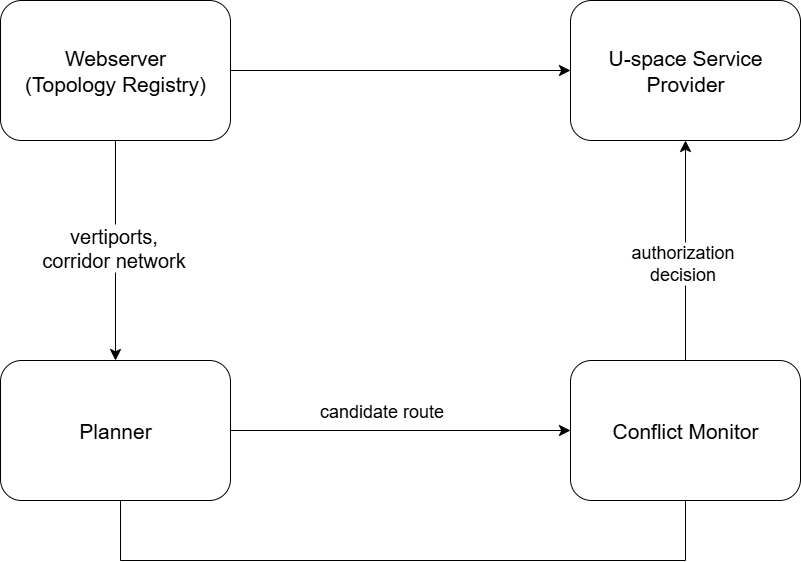
\includegraphics[width=0.5\textwidth]{figures/architecture.png}
  \caption{High-level architecture of the full-stack design. In the present implementation, the conflict-checking logic is embedded in the Planner.}
  \label{fig:architecture}
\end{figure}

  \chapter{Scenario and Data Basis}
\label{sec:scenario}

The path planning framework developed in this work is evaluated in a representative
urban environment: the metropolitan area of Hamburg. This scenario provides a dense
network of potential vertiports connected via corridors and reflects the kinds of
challenges expected in future urban air mobility (UAM) operations.


\section{Vertiports}
Vertiports represent the take-off and landing sites for eVTOL aircraft. In this
study, a set of anonymized vertiport locations within Hamburg is used. Each
vertiport may contain one or more landing pads; for analysis, the average
latitude and longitude of all pads is taken as the node coordinate.
Figure~\ref{fig:vertiports_hamburg} illustrates the spatial distribution of
these vertiports across the city.

\begin{figure}[H]
    \centering
    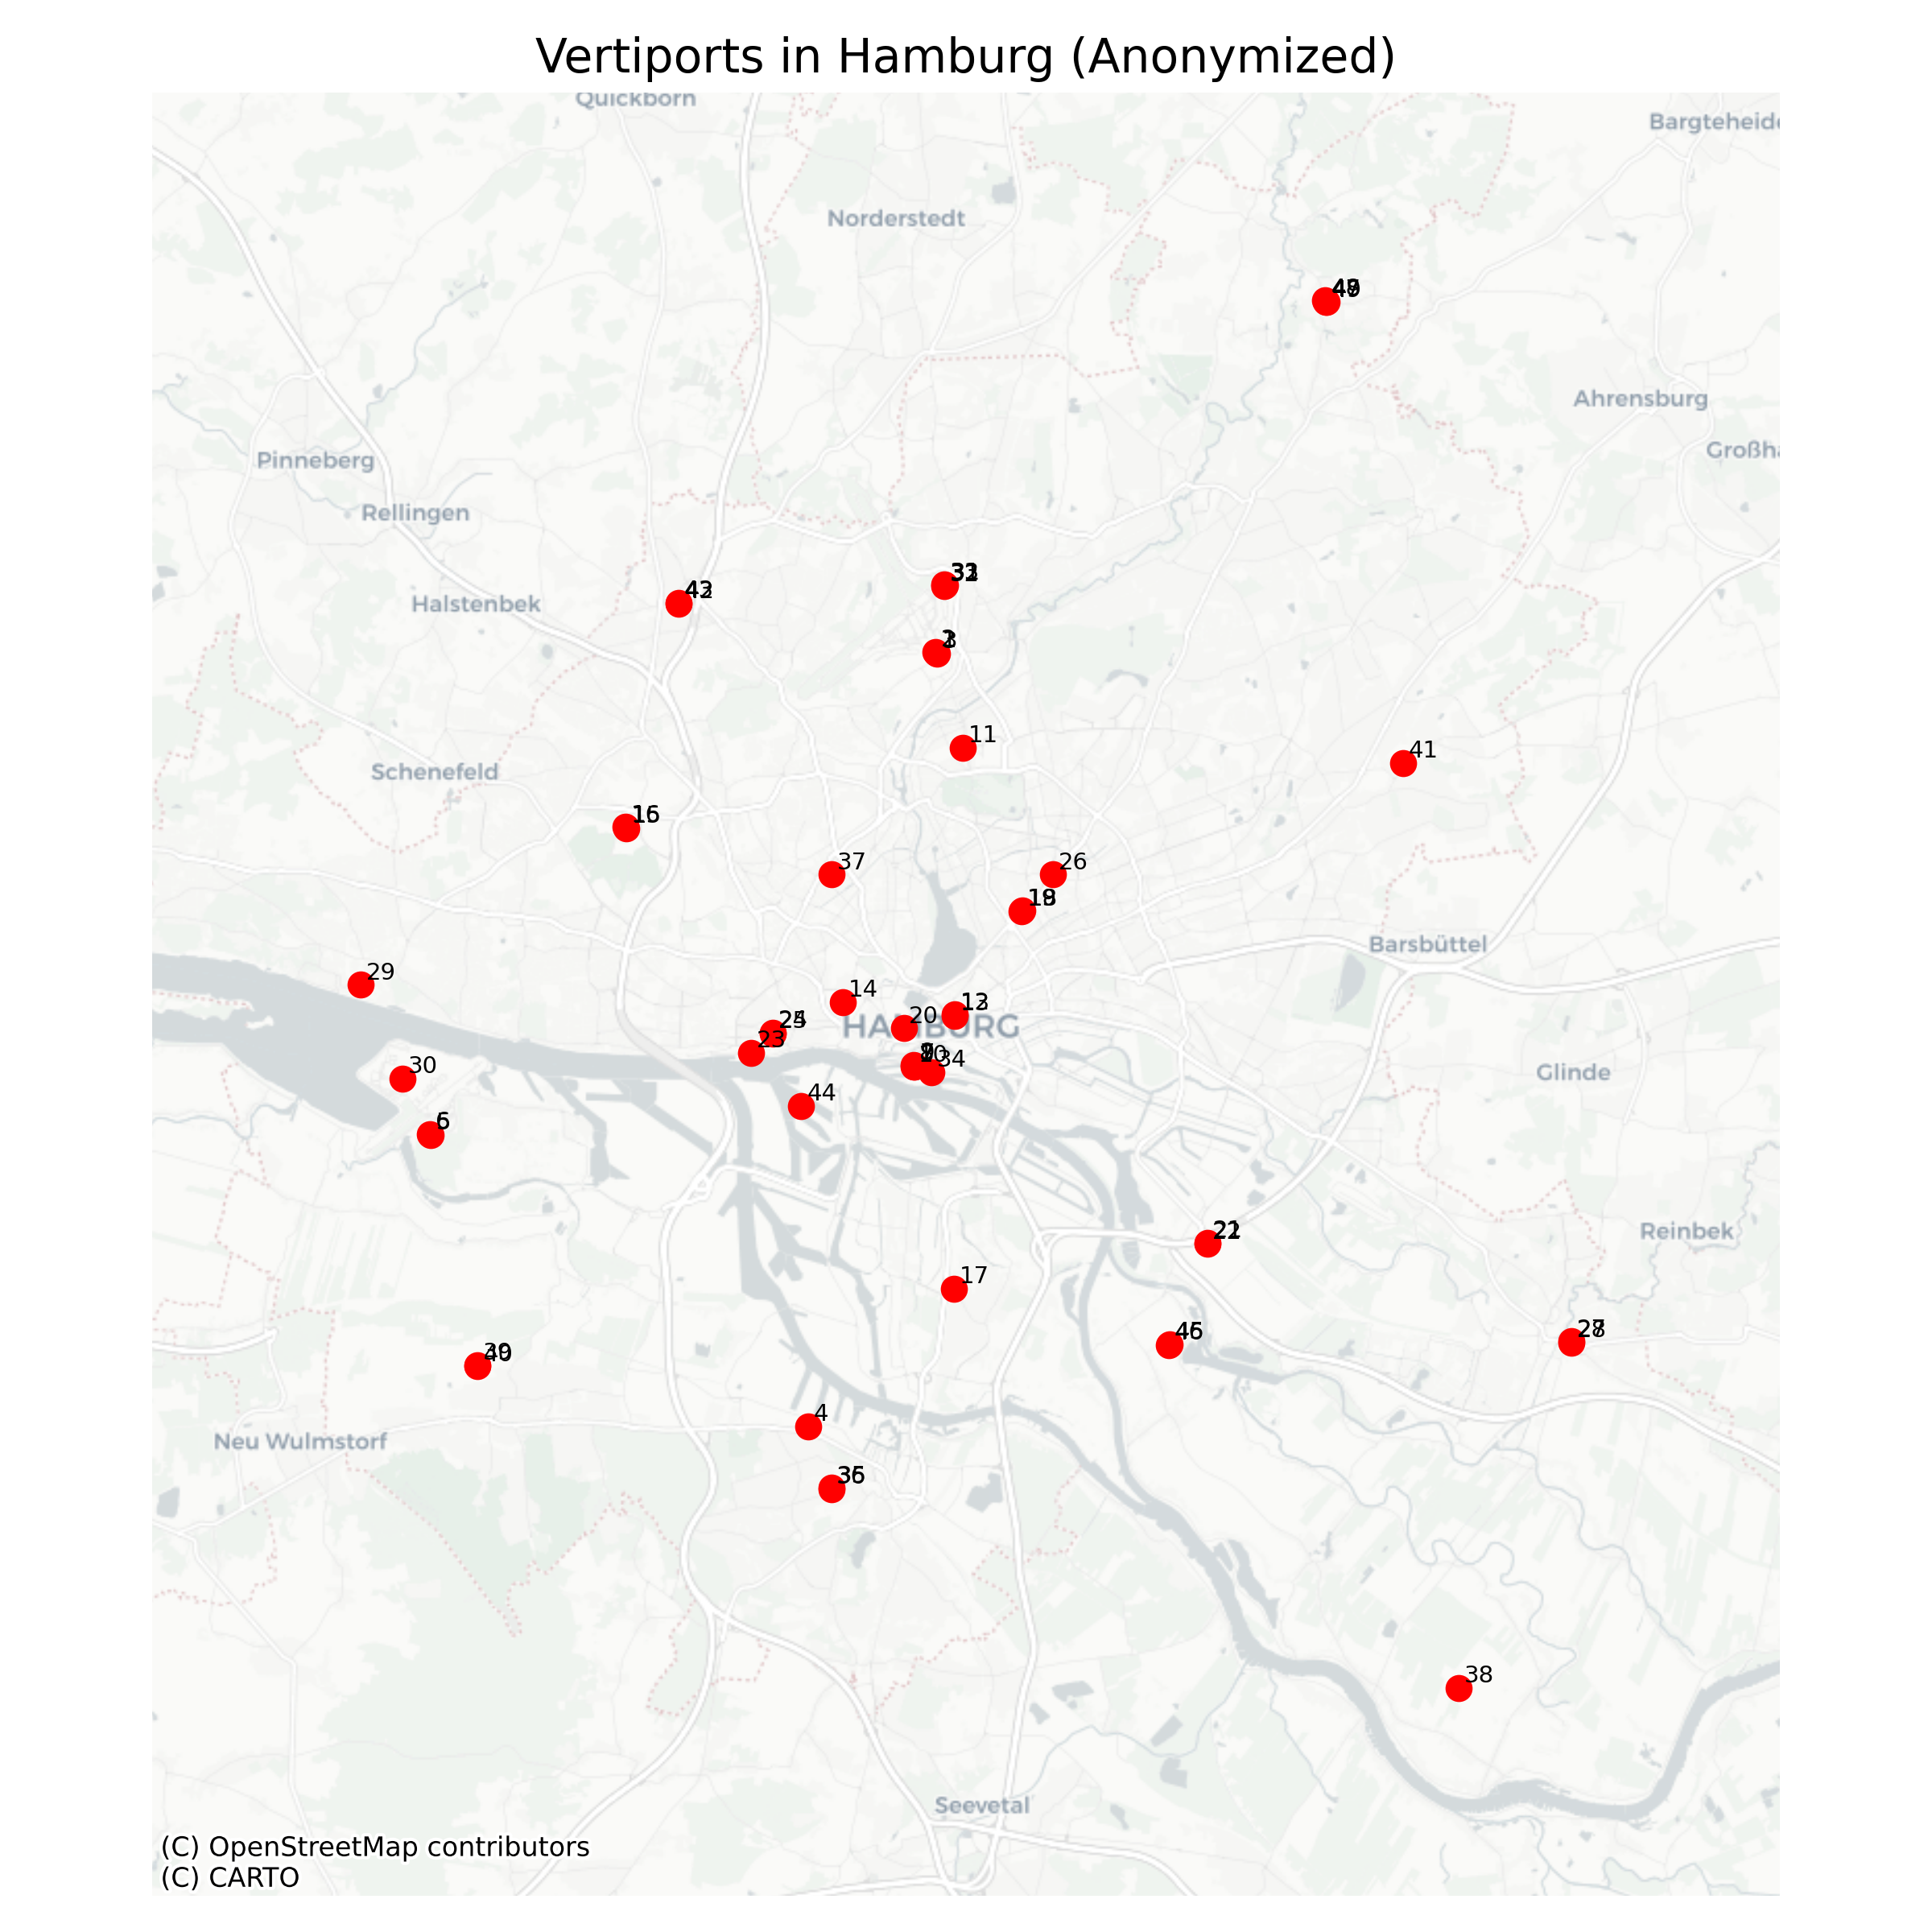
\includegraphics[width=0.8\textwidth]{figures/vertiports_hamburg.png}
    \caption{Vertiports in Hamburg (anonymized).}
    \label{fig:vertiports_hamburg}
\end{figure}

\subsection*{Corridors}
Corridors define the available airspace connections between vertiports and are
modeled as \emph{undirected} edges in the graph $G=(V,E)$. Geometrically, each
corridor is represented as a straight-line segment between two vertiports, and
the edge weight $d(u,v)$ corresponds to the geodesic (great-circle) distance
between their coordinates.

For the vertical structure, each corridor is placed at a fixed altitude layer.
According to the European Commission's U-space Blueprint \cite{eu_commission_2017},
a reference altitude of \SI{500}{ft} (approximately \SI{152}{m}) was adopted for
low-level airspace operations. In this work, a constant altitude of \SI{200}{m}
above ground level is used for the construction of corridors. Each corridor is
assigned a uniform width of \SI{20}{m}, representing a lateral safety buffer
around the nominal centerline.

For visualization and operator interaction, the corridor graph was also rendered in an interactive Cesium front-end (Fig. \ref{fig:corridors_comparison}, right). This allows the user to inspect the 3D geometry of the corridor network, vertical layering, and vertiport locations directly within a web-based interface.

Thus, the corridor model is characterized by the following specifications:
\begin{itemize}
    \item \textbf{Shape:} straight line between two vertiports;
    \item \textbf{Graph representation:} undirected edge with weight equal to geodesic distance;
    \item \textbf{Altitude:} constant \SI{200}{m} above ground level;
    \item \textbf{Width:} \SI{20}{m}.
\end{itemize}

\begin{figure}[H]
  \centering
  \begin{subfigure}{0.48\textwidth}
    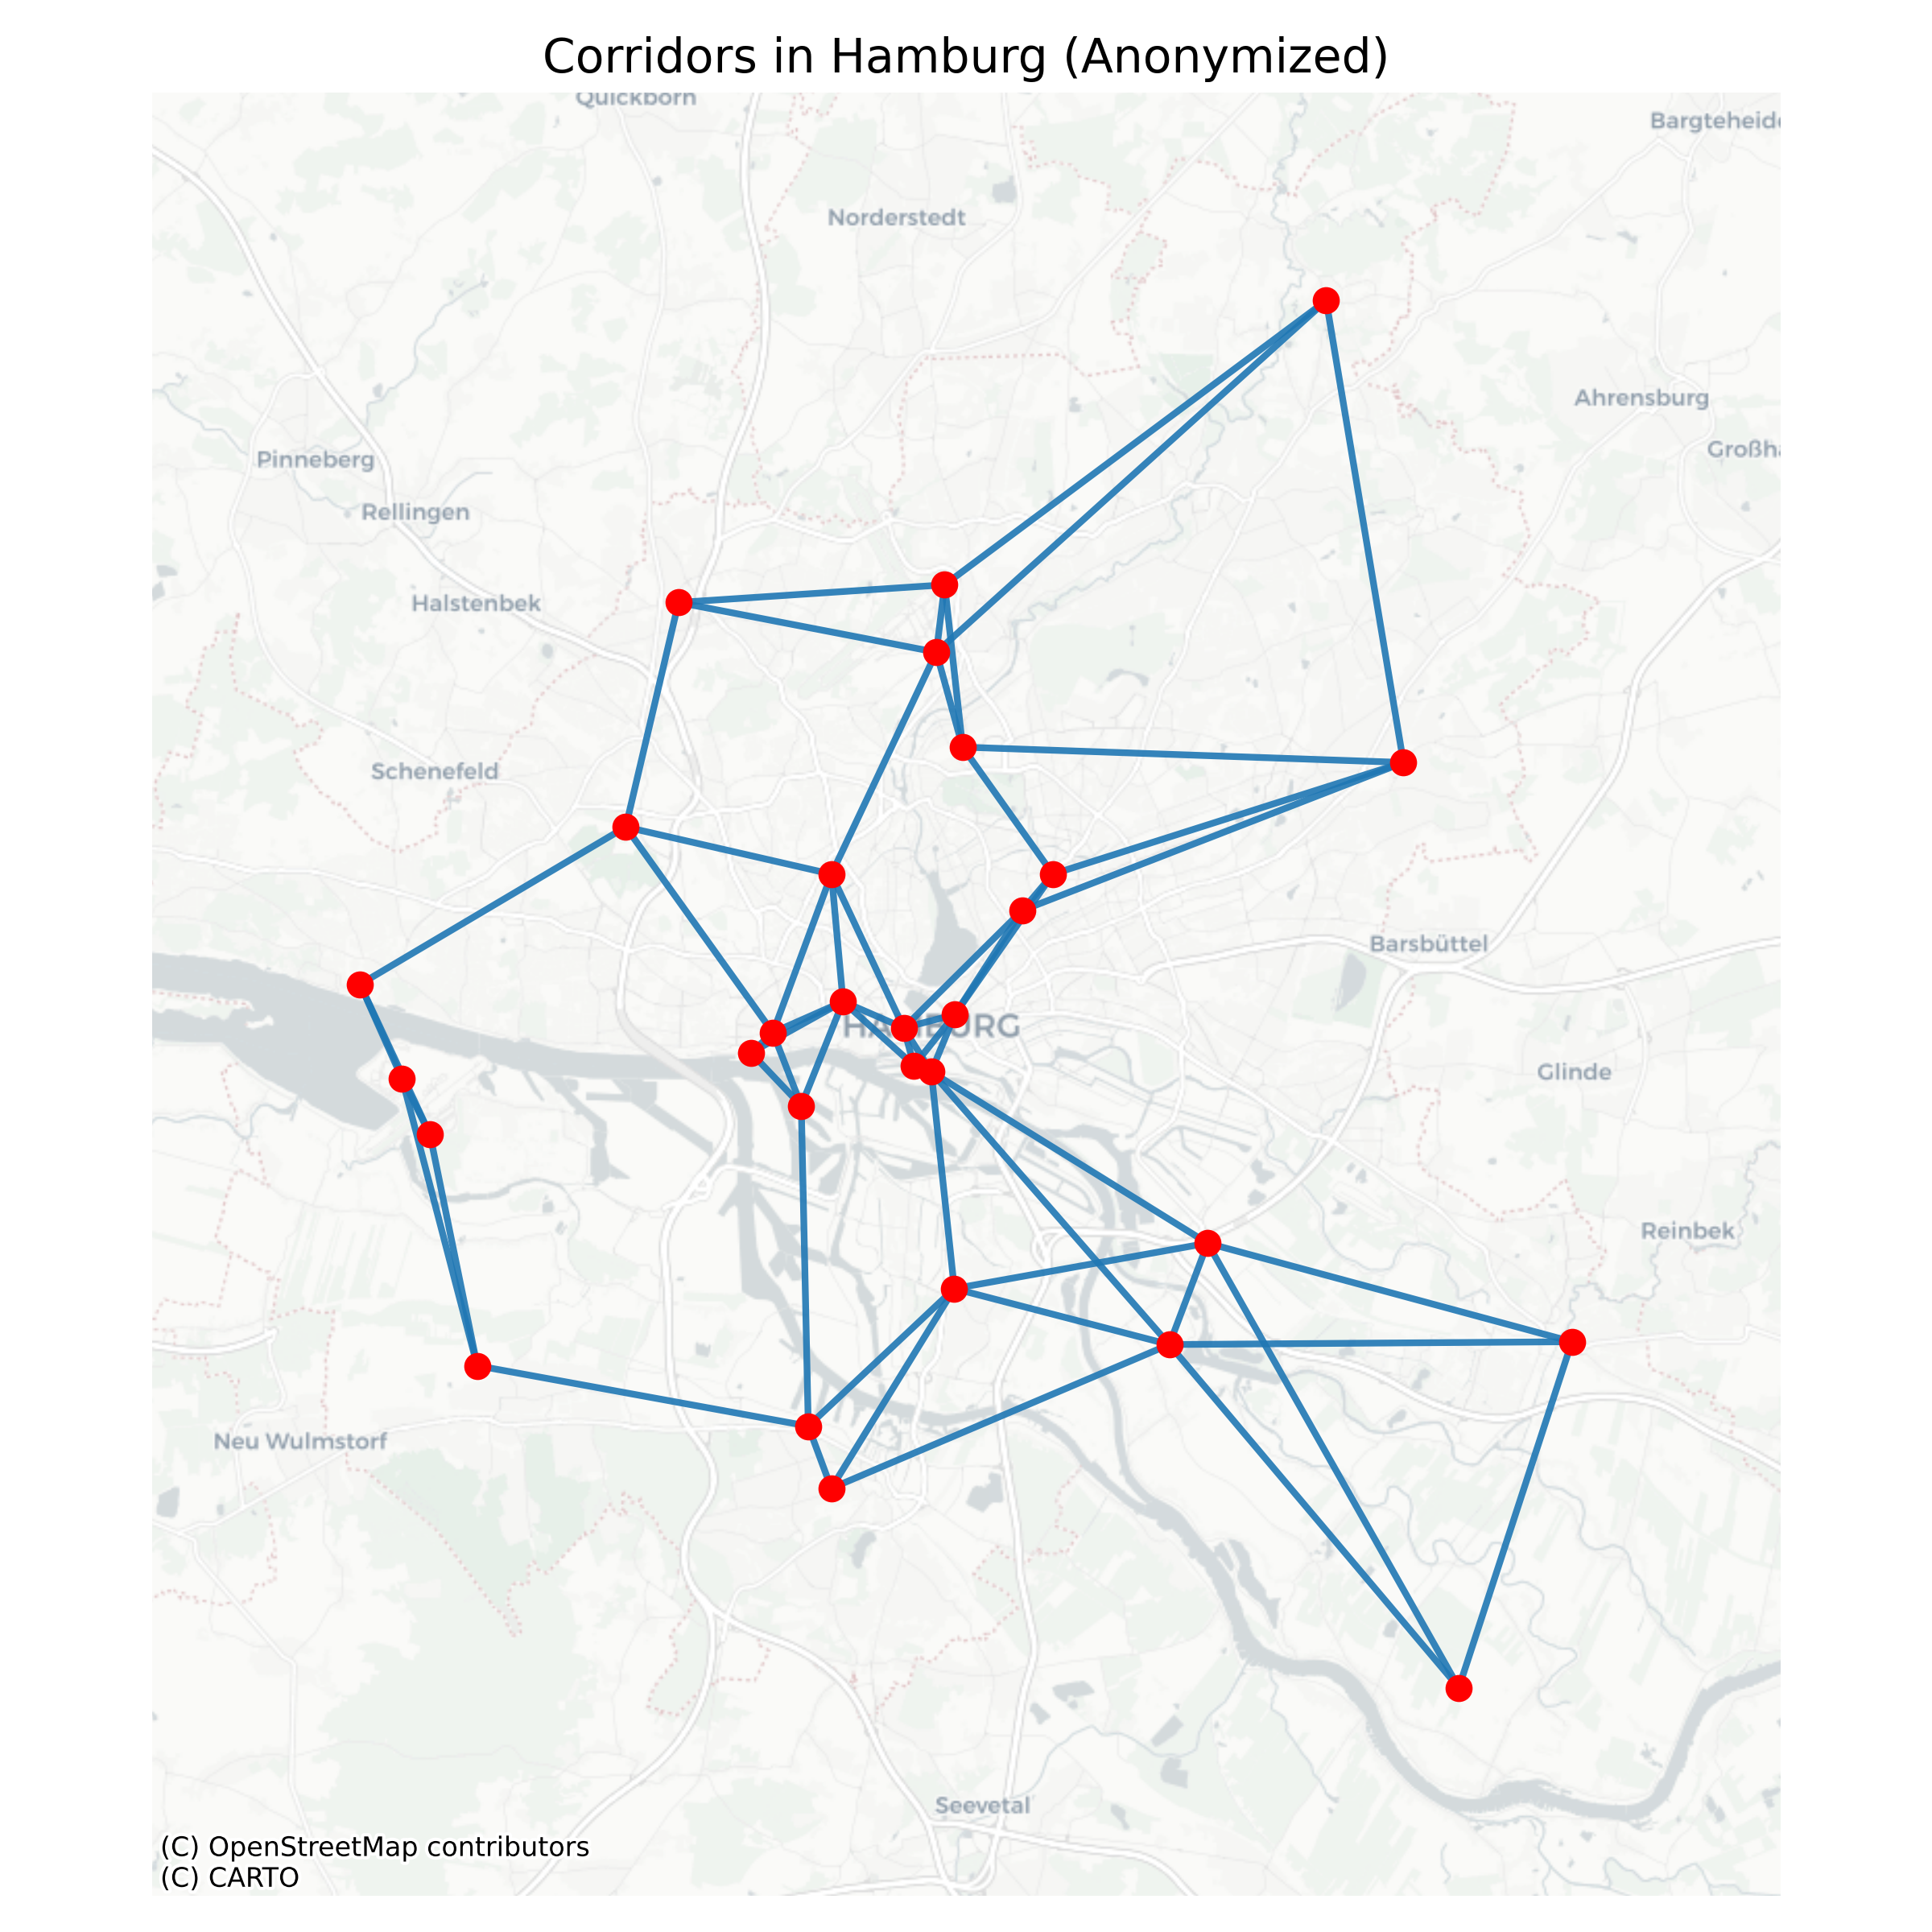
\includegraphics[width=\textwidth]{figures/corridors_hamburg.png}
    \caption{Constructed corridor network (static map view).}
    \label{fig:corridors_static}
  \end{subfigure}
  \hfill
  \begin{subfigure}{0.48\textwidth}
    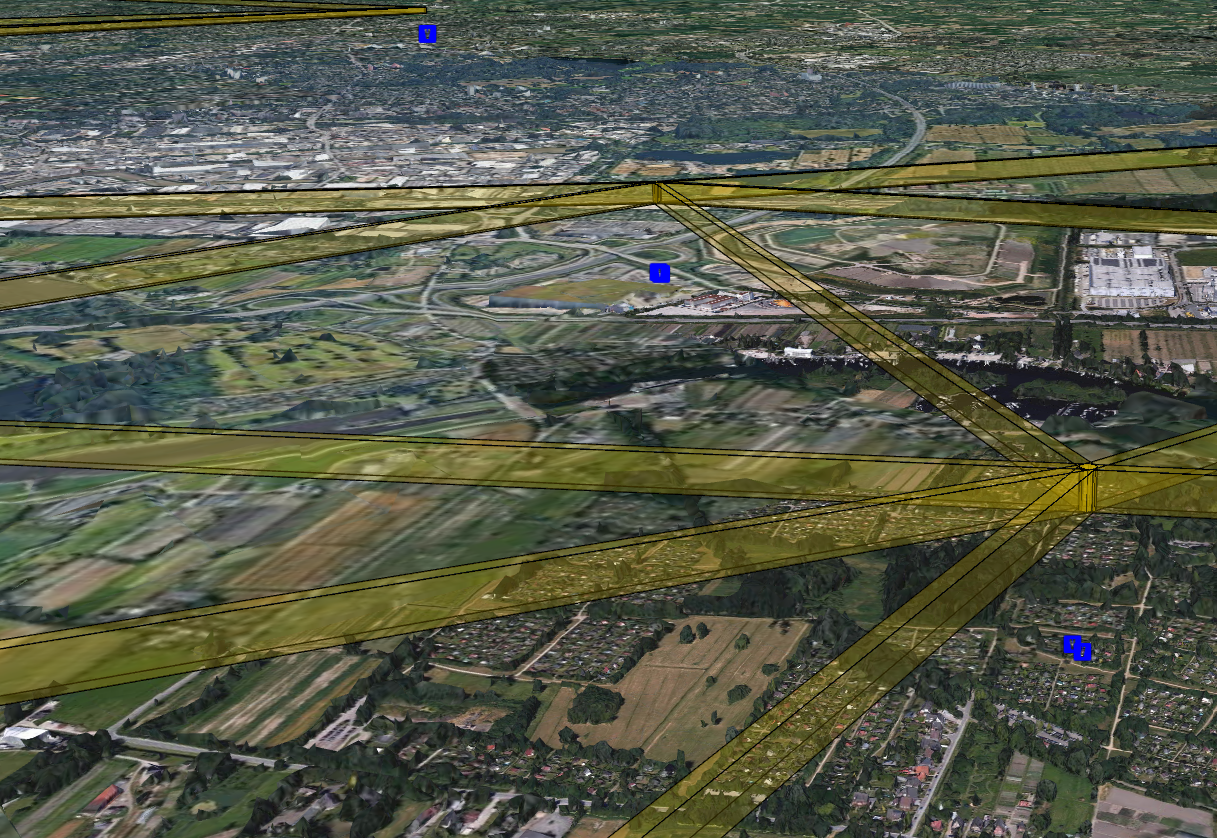
\includegraphics[width=\textwidth]{figures/corridors_hamburg_cesium.png}
    \caption{Cesium front-end view of the same corridor network (3D visualization).}
    \label{fig:corridors_cesium}
  \end{subfigure}
  \caption{Comparison of the corridor network in static map view (left) and interactive Cesium front-end (right).}
  \label{fig:corridors_comparison}
\end{figure}


\section{Graph Representation}
The resulting dataset is an \emph{undirected}, weighted graph in which nodes
correspond to vertiports and edges represent corridors. Edge weights are given
by geodesic distances between node coordinates. This graph serves as the basis
for all path planning experiments in this thesis; the global A* planner
(Sec.~\ref{sec:astar_global}) operates on this graph and uses the notation
$s$ (start), $n$ (current node), and $d$ (destination).

  \chapter{Path Planning Algorithms}%
\label{s_planning}

\section{Global A* Algorithm in Air Corridors}
\label{sec:astar_global}

For global path planning between vertiports, a graph search approach is adopted.
The urban airspace is modeled as an undirected, weighted graph where nodes
represent vertiports and edges represent available air corridors. The edge
weights are given by the geodesic distance between the connected vertiports,
computed using the Haversine formula. The planning objective is to determine the
shortest feasible route between a designated start and destination vertiport.

\subsection*{Problem Setup}
Let
\begin{itemize}
    \item $s \in V$ denote the starting vertiport,
    \item $d \in V$ denote the destination vertiport, and
    \item $n \in V$ denote a generic node (current vertiport) under expansion during the search.
\end{itemize}
The graph $G = (V,E)$ consists of a finite set of vertiports $V$ and undirected
edges $E \subseteq V \times V$, each edge $(u,v) \in E$ carrying a weight
$d(u,v)$ equal to the corridor distance between $u$ and $v$.

\subsection*{Illustration of the Search Graph}
\begin{figure}[H]
    \centering
    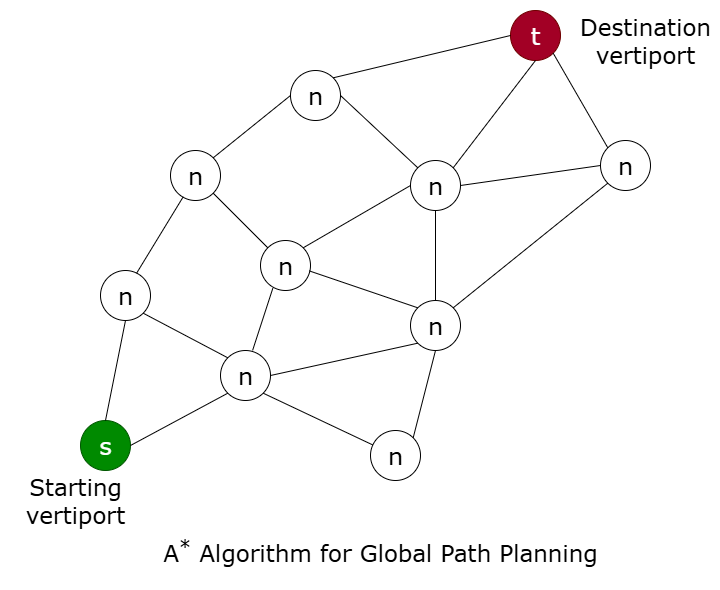
\includegraphics[width=0.6\textwidth]{figures/A_star.png}
    \caption{Illustration of the A* search on an undirected vertiport corridor graph.
    The starting node $s$ and destination node $d$ are connected through intermediate nodes $n$.}
    \label{fig:astar_graph}
\end{figure}

\subsection*{Heuristic}
To guide the A* search, the geodesic (Haversine) distance between the current
vertiport $n$ and the destination $d$ is used as the heuristic function $h(n)$.
Because the Haversine distance represents the shortest path on the Earth's
surface, it is admissible: the straight-line distance on the sphere is always
less than or equal to the length of any feasible path along the corridor
network.

Let $(\lambda_1,\varphi_1)$ and $(\lambda_2,\varphi_2)$ denote the longitude and
latitude (in radians) of the two points respectively. Define
$\Delta\varphi = \varphi_2 - \varphi_1$ and
$\Delta\lambda = \lambda_2 - \lambda_1$. Then the Haversine distance is given by

\begin{equation}
  d_\text{hav} = 2 R \arctan\!\Bigg(
  \frac{\sqrt{a}}{\sqrt{1-a}}\Bigg),
  \quad\text{with}\quad
  a = \sin^2\!\frac{\Delta\varphi}{2}
    + \cos\varphi_1 \cos\varphi_2
      \sin^2\!\frac{\Delta\lambda}{2},
\end{equation}

where $R$ is the Earth’s radius (here $R=\SI{6371}{km}$).

Accordingly, the heuristic function becomes
\begin{equation}
  h(n) = d_\text{hav}\big(\text{coord}(n), \text{coord}(d)\big),
\end{equation}
where $\text{coord}(v)$ denotes the geographic coordinates
$(\lambda,\varphi)$ of vertiport $v$.


\subsection*{Evaluation Function}
The total evaluation score for each node $n$ is defined as
\begin{equation}
    f(n) = g(n) + h(n),
\end{equation}
where $g(n)$ is the cumulative cost of the best-known path from $s$ to $n$, and
$h(n)$ is the heuristic estimate of the remaining cost to reach $d$.

In this context, the cost corresponds to the geodesic distance traveled along
the air corridors. Since the corridor network is assumed to operate at a fixed
altitude layer, the planning problem reduces to two dimensions, and the distance
is computed purely in terms of latitude and longitude. Thus, $g(n)$ accumulates
the 2D distances of all corridor segments from the start to the current node,
while $h(n)$ provides the straight-line (Haversine) estimate from the current
node to the destination. The evaluation score $f(n)$ therefore balances the actual
distance traveled so far with an optimistic estimate of the remaining distance,
ensuring efficient convergence toward the destination.

\subsection*{Algorithm}
The algorithm used is the classical A* search, adapted to the vertiport
corridor graph. It maintains a priority queue of nodes to be expanded,
ordered by their $f(n)$ value.

\begin{algorithm}[H]
\caption{A* Path Planning in Air Corridors}
\label{alg:astar}
\begin{algorithmic}[1]
\Require Start vertiport $s$, destination vertiport $d$, undirected graph $G = (V, E)$ with edge distances $d(u,v)$, coordinates $\text{coord}(v)$
\Ensure Sequence of vertiports representing the planned route
\State $open \gets \{s\}$ \Comment{priority queue with key $f(v)$}
\State $came\_from \gets \emptyset$
\State $g(s) \gets 0$
\State $f(s) \gets h(s) =$ Haversine$(\text{coord}(s), \text{coord}(d))$
\While{$open$ not empty}
  \State $current \gets \arg\min_{v \in open} f(v)$
  \If{$current = d$}
    \State \Return Reconstruct path from $came\_from$
  \EndIf
  \State Remove $current$ from $open$
  \ForAll{$neighbor \in$ neighbors($current$)}
    \State $tentative\_g \gets g(current) + d(current, neighbor)$
    \If{$tentative\_g < g(neighbor)$}
      \State $came\_from[neighbor] \gets current$
      \State $g(neighbor) \gets tentative\_g$
      \State $h(neighbor) \gets$ Haversine$(\text{coord}(neighbor), \text{coord}(d))$
      \State $f(neighbor) \gets g(neighbor) + h(neighbor)$
      \State Add $neighbor$ to $open$
    \EndIf
  \EndFor
\EndWhile
\State \Return failure (no path found)
\end{algorithmic}
\end{algorithm}

\subsection*{Output}
The algorithm returns the ordered list of vertiports
\begin{equation}
    \{ s, v_1, v_2, \dots, d \},
\end{equation}

that the aircraft should traverse. These nodes represent intermediate waypoints
along the air corridor network and form the global reference trajectory for
subsequent local planning and trajectory generation.

\section{Trajectory Generation Pipeline}
\label{s_traj_generation}

This section describes the generation of four–dimensional (4D) urban air mobility (UAM) trajectories
(latitude, longitude, altitude, time).This pipeline interfaces with the C++-based CFMS \cite{morscheck2021cfms} system while the planner is implemented in Python, demonstrating the microservice concept of this work. The pipeline transforms a discrete path over the vertiport
network into a kinematically consistent, phase–annotated trajectory by (i) synthesizing geometric
waypoints, (ii) assigning vertical and speed constraints, and (iii) invoking a modular flight
management and 4D trajectory generation system (CFMS) \cite{morscheck2021cfms} to densify and
time–parameterize the path.

\subsection{Notation and Conventions}
\label{s:traj_notation}

The following symbols and units are used throughout this work:
\begin{itemize}
  \item \textbf{Path over the graph:} $P = [v_0, v_1, \dots, v_n]$ is the ordered list of
  vertiports yielded by the global A* planner (Sec.~\ref{sec:astar_global}), with $v_0 = s$ (start)
  and $v_n = d$ (destination).

  \item \textbf{Coordinates:} each vertiport $v_i$ is associated with WGS–84 coordinates
  $\mathcal{V}(v_i) = (\varphi_i, \lambda_i, h_i)$ with
  latitude $\varphi_i$ (degrees), longitude $\lambda_i$ (degrees), and pad elevation $h_i$ (meters, MSL).

  \item \textbf{Altitude variables:} In this study, corridors are modelled at a fixed
    absolute altitude layer of \(H_{\text{corridor}}=\SI{200}{m}\) above mean sea level,
    independent of individual pad elevations. All cruise waypoints are therefore
    generated at this fixed altitude:
    \begin{equation}
        H^{\text{abs}} \;=\; H_{\text{corridor}}
    \end{equation}
    while take-off and landing waypoints use the actual pad elevation \(h_i\), and
    intermediate climb/descent waypoints interpolate between \(h_i\) and \(H_{\text{corridor}}\).

  \item \textbf{Time:} continuous time is denoted by $\tau$ (seconds). This symbol is used
  consistently in equations to represent elapsed time along a trajectory.

  \item \textbf{Geodesic distance:} $d(u,v)$ is the great-circle distance between two coordinates
  (Haversine).

  \item \textbf{Linear interpolation:} $\mathrm{lerp}(a,b,\alpha) \coloneqq a + (b-a)\,\alpha$, for $\alpha\in[0,1]$.
\end{itemize}


\subsection{Inputs}
The following inputs are used for the trajectory generation stage:

\begin{itemize}
  \item Path $P = [v_0, v_1, \dots, v_n]$ from A* (Sec.~\ref{sec:astar_global}).
  \item Vertiport map $\mathcal{V}: v_i \mapsto (\varphi_i, \lambda_i, h_i)$ (deg, deg, m MSL).
  \item Requested cruise height $H_c$ (AGL), default \SI{200}{m}.
  \item UAM speed profile with safety margin.
\end{itemize}

To ensure that the generated 4D trajectory remains flyable even under moderate disturbances 
(e.g.\ wind gusts, small deviations, or delayed responses), the nominal speeds used in this study 
are derived from the aircraft’s maximum performance values multiplied by a safety factor 
\(s_{\text{f}}\in(0,1)\).  
For the reference UAM vehicle the maximum performance limits are

\[
\begin{aligned}
    V_{\text{takeoff,max}}   &= \SI{0}{m/s}, \quad
    V_{\text{transition,max}} &= \SI{20}{m/s}, \\
    V_{\text{cruise,max}}     &= \SI{30}{m/s}, \quad
    V_{\text{approach,max}}   &= \SI{20}{m/s}.
\end{aligned}
\]

Applying a safety factor of \(s_{\text{f}}=0.75\) yields the nominal speeds adopted in the planning process:

\[
\begin{aligned}
    V_{\text{takeoff}}   &= s_{\text{f}}\;V_{\text{takeoff,max}} = \SI{0}{m/s}, \qquad
    V_{\text{transition}} &= s_{\text{f}}\;V_{\text{transition,max}} = \SI{15}{m/s},\\[0.5em]
    V_{\text{cruise}}    &= s_{\text{f}}\;V_{\text{cruise,max}} = \SI{25}{m/s}, \qquad
    V_{\text{approach}}  &= s_{\text{f}}\;V_{\text{approach,max}} = \SI{15}{m/s}.
\end{aligned}
\]


These safety-factored speeds are used as the target values for the 
\texttt{UAM\_takeoff}, \texttt{cruise} and \texttt{UAM\_landing} phases when 
annotating the waypoints.


\subsection{Waypoint Synthesis}
Given $P$, the waypoint generator produces an ordered list $W = [w_1,\dots,w_m]$ where each waypoint is
\begin{equation}
  w_k \;=\; \{\varphi_k, \lambda_k, H_k, \texttt{id}, \texttt{(optional) speed\_reduction}\}.
\end{equation}
The construction logic is as follows:
\begin{enumerate}
  \item \textbf{Initial takeoff point:} at $(\varphi_0,\lambda_0,h_0)$.
  \item \textbf{Mid–climb point:} along the initial bearing $v_0 \rightarrow v_1$ at
        \(\alpha=0.3\) of the segment, with altitude
        \begin{equation}
          H_{\text{climb}} \;=\; h_0 + 0.6\,(H^{\text{abs}} - h_0).
        \end{equation}
  \item \textbf{Cruise nodes at internal vertiports:} for each $v_i,\, i=1,\dots,n-1$,
        altitude is set to $H^{\text{abs}}$.
  \item \textbf{Pre–landing descent point:} along $v_{n-1} \rightarrow v_n$ at \(\alpha=0.7\)
        with
        \begin{equation}
          H_{\text{descent}} \;=\; h_n + 0.7\,(H^{\text{abs}} - h_n).
        \end{equation}
        This intermediate waypoint provides a clear transition from cruise altitude
        to the terminal approach. It produces a two-stage vertical profile
        (cruise $\rightarrow$ descent $\rightarrow$ landing) that smooths vertical-rate changes,
        yields more realistic trajectories, and leaves adequate horizontal distance
        for deceleration and stabilization before touchdown. The value
        \(\alpha=0.7\) is a simple, tunable heuristic chosen to begin the descent
        early enough for comfortable flare and speed control while preserving
        lateral fidelity.

  \item \textbf{Final landing point:} at $(\varphi_n,\lambda_n,h_n)$.
\end{enumerate}


\subsection{Phase Encoding and Speed Constraints}
Each waypoint is annotated with a nominal flight phase and target speed:

\begin{description}
  \item[\texttt{UAM\_takeoff}] Initial (pad) waypoint, executed at the takeoff speed \(V_{\text{takeoff}}\).
  \item[\texttt{cruise}] Mid–climb, internal cruise nodes, and descent–initiation nodes,
  with \(V_{\text{transition}}\) applied at climb/descent anchors and \(V_{\text{cruise}}\) along the en-route segments.
  \item[\texttt{UAM\_landing}] Final (pad) waypoint, with the speed set to \(0\,\text{m/s}\) (stationary at landing).
\end{description}


\subsection{CFMS Integration}
The waypoint list is converted to the CFMS input structure:
\begin{itemize}
  \item $(\varphi,\lambda)$ converted from degrees to radians.
  \item Altitudes expressed in meters MSL (using $H^{\text{abs}}$ for cruise waypoints).
  \item Phase and speed fields set as above; the global context specifies the aircraft type
  \texttt{CFMS\_UAMcopter}, cruise height $H_c$, and cruise speed $V_{\text{cruise}}$.
\end{itemize}
CFMS \cite{morscheck2021cfms} then generates a dense 4D trajectory
\(\mathcal{T} = \{(\varphi(\tau), \lambda(\tau), H(\tau), \tau, \dots)\}\) that satisfies the kinematic
profile and phase schedule.

\subsection{Temporal and Spatial Sampling}
To reduce data volume, the CFMS output is uniformly sub–sampled to at most $M=500$ points:
\begin{equation}
  \mathrm{index}_i \;=\; \left\lfloor \frac{i\,(N-1)}{M-1} \right\rfloor,\quad i=0,\dots,M-1,
\end{equation}
with $N$ original samples; the first and last samples are always retained.

\subsection{Exported Data Fields}
Each trajectory is represented as a sequence of sampled data points of the form
\begin{equation}
\{\varphi,\lambda,H,\texttt{t},\text{TAS},V_g,\phi,\dot{H},\dot{\psi},\texttt{flight\_phase}\},
\end{equation}
where:
\begin{itemize}
  \item $\varphi$ – latitude of the sample point (deg).
  \item $\lambda$ – longitude of the sample point (deg).
  \item $H$ – altitude above mean sea level (m).
  \item \texttt{t} – elapsed time since the start of the trajectory (s); denoted by $\tau$ in the equations.
  \item \text{TAS} – true airspeed (m/s): the speed of the vehicle relative to the surrounding air.
  \item $V_g$ – ground speed (m/s): magnitude of the velocity vector relative to the ground.
  \item $\phi$ – bank angle (deg): roll about the longitudinal axis; zero is wings-level.
  \item $\dot{H}$ – climb rate (m/s): time derivative of altitude; positive in climb, negative in descent.
  \item $\dot{\psi}$ – turn rate (deg/s): rate of change of the ground-track angle.  
  In coordinated flight it can be approximated by
  \begin{equation}
    \dot{\psi} \;=\; \frac{g\,\tan\phi}{V_g},
  \end{equation}
  where $g$ is gravitational acceleration (m/s$^2$).
  \item \texttt{flight\_phase} – label indicating the nominal phase of flight:
    \texttt{UAM\_takeoff} (departure and climb), 
    \texttt{cruise} (en-route), 
    \texttt{UAM\_landing} (approach and landing), or 
    \texttt{other} (any intermediate or internal phase).
\end{itemize}


\subsection{Algorithm Summary}
\begin{algorithm}[H]
\caption{Trajectory Generation from A* Path}
\label{alg:traj_gen}
\begin{algorithmic}[1]
\Require Path $P=[v_0,\dots,v_n]$, vertiport map $\mathcal{V}$, cruise height $H_c$ (AGL)
\Ensure Subsampled, phase–annotated 4D trajectory $\mathcal{T}'$
\State $H^{\text{abs}} \gets h_0 + H_c$ \Comment{constant cruise layer above departure pad}
\State $W \gets$ synthesize\_waypoints$(P,\mathcal{V},H^{\text{abs}})$
\State annotate phases and speeds in $W$ (\texttt{UAM\_takeoff}, \texttt{cruise}, \texttt{UAM\_landing})
\State $W_{\text{CFMS}} \gets$ convert\_to\_CFMS$(W)$ \Comment{radians; altitudes in m MSL}
\State $\mathcal{T} \gets$ CFMS\_generate\_trajectory$(W_{\text{CFMS}})$
\State $\mathcal{T}' \gets$ uniform\_subsample$(\mathcal{T}, M=500)$
\State export $\mathcal{T}'$ as JSON $\{\varphi,\lambda,H,\texttt{t},\dots\}$
\end{algorithmic}
\end{algorithm}

\paragraph{Consistency with Global Planning.}
The global A* planner (Sec.~\ref{sec:astar_global}) minimizes 2D geodesic distance over the corridor
graph at a fixed altitude layer. The trajectory pipeline respects this assumption by assigning a
constant cruise height $H_c$ (AGL) along the route and applying geodesic distances only for horizontal planning.

\section{Conflict Detection with NDMap}
\label{sec:ndmap}

The following section is a summarized version of the NDMap conflict detection method presented in \cite{NDMap}, adapted to the requirements of this work.

\subsection*{Overview}
In this work, conflicts are detected using NDMap configured in four dimensions
\((\lambda,\varphi,H,\tau)\), i.e., longitude \([\mathrm{deg}]\), latitude \([\mathrm{deg}]\), altitude \([\mathrm{m}]\), and time \([\mathrm{s}]\).
NDMap indexes submitted trajectories in this 4D space and, for a newly inspected trajectory,
efficiently identifies portions of previously submitted trajectories that come within
user-defined separation minima. This enables very fast screening suitable for near real-time admission control.

\subsection*{Inputs and Configuration}
Each trajectory is represented as an ordered sequence of sampled four-dimensional points
\[
(\lambda,\varphi,H,\tau)
\;\in\;
[-180^\circ,180^\circ] \times [-90^\circ,90^\circ] \times [0,100000]~\text{m} \times [0,86400]~\text{s},
\]
where  
$\lambda$ is longitude (deg),  
$\varphi$ is latitude (deg),  
$H$ is altitude above mean sea level (m), and  
$\tau$ is time (s).

Separation requirements are encoded as a vector
\begin{equation}
  \mathbf{S} \;=\; 
  \bigl(\Delta\lambda_{\min},\,\Delta\varphi_{\min},\,\Delta H_{\min},\,\Delta\tau_{\min}\bigr),
\end{equation}
which sets the minimum allowed spacing in each dimension and parameterizes the detector’s resolution.  
In this study,
\[
\mathbf{S} = 
\bigl(0.002^\circ,\;0.004^\circ,\;300~\text{m},\;90~\text{s}\bigr),
\]
corresponding respectively to minimum separations in longitude (deg), latitude (deg), altitude (m), and time (s).  
A minimum inter-conflict interval of \(2~\text{s}\) is applied to merge very closely spaced detections.

\subsection*{Output}
For each conflicting pair involving the inspected trajectory, NDMap returns one or more
\emph{conflict time intervals}
\[
[\tau_{\text{start}},\,\tau_{\text{end}}],
\]
expressed in seconds on the scenario time axis. These intervals constitute the primary output consumed
by the deconfliction/scheduling logic in this work.

\subsection*{Performance Characteristics}
According to the NDMap documentation \cite{NDMap}, runtimes are on the order of
milliseconds per trajectory on commodity hardware, with reported averages of a few milliseconds per
object for national- to continental-scale datasets. The implementation exhibits near-linear scaling
with dataset size and tunable trade-offs between runtime and memory via configuration parameters, which
supports near real-time screening in the intended UAM use case.

\medskip
\noindent\textbf{Summary.}
NDMap consumes sampled 4D trajectories together with separation minima \(\mathbf{S}\) and produces
conflict time intervals \([\tau_{\text{start}},\tau_{\text{end}}]\) for any violations. The detector’s
low latency and favorable scaling make it appropriate for iterative, online conflict checks within
the planning pipeline described in this thesis.

\section{Conflict Resolution}
\label{sec:conflict_resolution}

Conflict detection with NDMap (Sec.~\ref{sec:ndmap}) identifies spatio-temporal overlaps 
between a newly proposed candidate trajectory and the set of already submitted trajectories. 
To ensure conflict-free operation, conflict resolution is applied directly within the 
path planning loop of this work.

\subsection*{Resolution Strategy}
In this study, conflict resolution is realized through \textbf{lateral re-routing}. 
The principle is to discourage the reuse of route segments that are involved in conflicts 
and to force the planner to search for an alternative path through the corridor network.

\begin{enumerate}
    \item A candidate path is computed using the global A* planner (Sec.~\ref{sec:astar_global}).
    \item The corresponding trajectory is generated and checked against existing traffic using NDMap.
    \item If a conflict is detected, the edges of the corridor graph that belong to the conflicting candidate route are penalized by 
    assigning them effectively infinite weight, i.e.,
    \[
      d(u,v) \;\coloneqq\; \infty, \quad \forall\,(u,v)\in E_{\text{conflict}},
    \]
    which removes them from further consideration by A*.
    \item A* is re-executed on the modified graph to find an alternative route that avoids the discouraged edges.
    \item This process is repeated iteratively until NDMap no longer reports conflicts.
\end{enumerate}

\subsection*{Properties}
This integrated resolution approach has the following characteristics:
\begin{itemize}
    \item \textbf{Simplicity:} implemented as an extension of the global A* search without requiring additional modules.
    \item \textbf{Determinism:} the iterative penalization guarantees that once all conflicting edges are discouraged, 
    the resulting solution is conflict-free (if a feasible route exists).
    \item \textbf{Cost trade-off:} since conflicts are avoided by forbidding certain edges, 
    the resulting route may be longer than the original candidate, reflecting a trade-off between efficiency and safety.
    \item \textbf{Scalability:} the conflict detection and re-routing loop can be repeated for successive trajectory submissions, 
    enabling online admission control in multi-UAV settings.
\end{itemize}

\subsection*{Scope of this Work}
Although other resolution mechanisms such as temporal shifting or vertical maneuvering 
are possible, the present work focuses exclusively on lateral re-routing within the 
corridor graph. This allows for a modular and scalable demonstration of how conflict 
detection (via NDMap) and path planning (via A*) can be tightly integrated in a unified framework.

\begin{figure}[H]
    \centering
    \begin{subfigure}{0.45\textwidth}
        \centering
        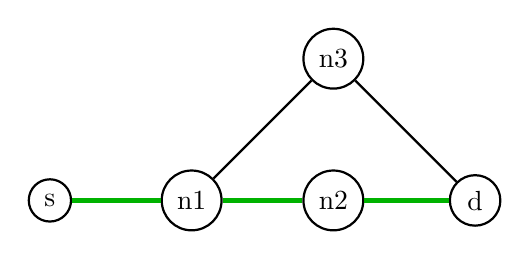
\begin{tikzpicture}[node distance=1.8cm,thick]
            % Nodes
            \node[circle,draw] (s) {s};
            \node[circle,draw,right of=s] (a) {n1};
            \node[circle,draw,right of=a] (b) {n2};
            \node[circle,draw,right of=b] (d) {d};
            \node[circle,draw,above of=b] (c) {n3};

            % Edges
            \draw (s) -- (a);
            \draw (a) -- (b);
            \draw (b) -- (d);
            \draw (a) -- (c) -- (d);

            % Path
            \draw[green!70!black,ultra thick] (s) -- (a) -- (b) -- (d);
        \end{tikzpicture}
        \caption{Initial candidate path (green).}
    \end{subfigure}
    \hfill
    \begin{subfigure}{0.45\textwidth}
        \centering
        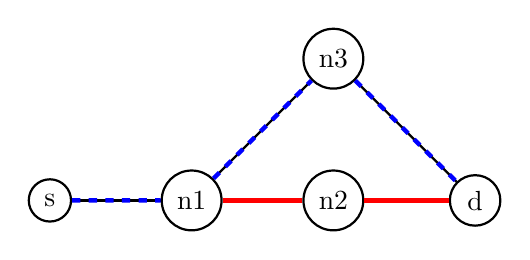
\begin{tikzpicture}[node distance=1.8cm,thick]
            % Nodes
            \node[circle,draw] (s) {s};
            \node[circle,draw,right of=s] (a) {n1};
            \node[circle,draw,right of=a] (b) {n2};
            \node[circle,draw,right of=b] (d) {d};
            \node[circle,draw,above of=b] (c) {n3};

            % Edges
            \draw (s) -- (a);
            \draw (a) -- (b);
            \draw (b) -- (d);
            \draw (a) -- (c) -- (d);

            % Conflict edges
            \draw[red,ultra thick] (a) -- (b);
            \draw[red,ultra thick] (b) -- (d);

            % New path
            \draw[blue,ultra thick,dashed] (s) -- (a) -- (c) -- (d);
        \end{tikzpicture}
        \caption{Conflict edges penalized (red), re-routed path (blue dashed).}
    \end{subfigure}
    \caption{Illustration of conflict resolution via lateral re-routing.}
    \label{fig:conflict_resolution}
\end{figure}



  \chapter{Results}
\label{s_results}

This chapter presents the results of the path planning framework developed in this work. 
It reports representative trajectories between selected vertiports in the Hamburg scenario (Sec.~\ref{sec:scenario}), 
the associated kinematic profiles (true airspeed, turn rate, altitude, bank angle), 
geometric properties of the paths, and computational performance for planning and trajectory generation 
(Secs.~\ref{sec:astar_global} and \ref{s_traj_generation}). 
A dedicated section (Sec.~\ref{sec:results_conflicts}) demonstrates conflict detection outcomes using NDMap (method in Sec.~\ref{sec:ndmap}).

\medskip
\noindent
All trajectories and profiles shown in this chapter are \emph{planned (reference) 4D trajectories} produced by the pipeline, i.e., the intended paths to be followed by the aircraft; they are not simulation runs.

\section{Experimental Setup}
\label{sec:results_setup}

\subsection{Scenario and Data}
The experiments are conducted on the Hamburg vertiport network described in Sec.~\ref{sec:scenario}, 
with corridors modeled as undirected edges at a constant altitude layer of \SI{200}{m} AGL and width \SI{20}{m}. 
Nodes correspond to vertiports (averaged pad coordinates); edges are weighted by geodesic distance.

\subsection{Planner and Generator Configuration}
\begin{itemize}
  \item \textbf{Global planner:} A* on the undirected corridor graph (Sec.~\ref{sec:astar_global}), with Haversine heuristic \(h(n)\) and evaluation function \(f(n)=g(n)+h(n)\).
  \item \textbf{Trajectory generator:} CFMS-based 4D trajectory synthesis (Sec.~\ref{s_traj_generation}) with cruise height \(H_c=\SI{200}{m}\) (AGL), speed profile \((V_{\text{takeoff}}, V_{\text{transition}}, V_{\text{cruise}}, V_{\text{approach}})\).
\end{itemize}

\subsection{Evaluation Metrics}
The following metrics are reported for each run:
\begin{itemize}
  \item \textbf{Path geometry:} number of legs, total length \(L\) (km).
  \item \textbf{Timing:} total flight time \(T\) (s), average TAS.
  \item \textbf{Kinematics:} TAS profile, altitude compliance w.r.t.\ \(H_c\), peak bank angle \(\max \phi\), peak turn rate \(\max \dot{\psi}\).
  \item \textbf{Compute:} A* runtime and trajectory generation time.
\end{itemize}

\section{Case Studies: Sample Trajectories}
\label{sec:results_case_studies}

This section presents representative trajectories between selected vertiport pairs. 
For each case, \(s\) denotes the starting vertiport and \(d\) the destination.

\subsection{Representative Long-Leg Route}
\label{sec:trajA}

Trajectory A was selected as a representative case because it contains one of the longest legs in the Hamburg network. 
This results in a comparatively high total path length and flight time. 
Furthermore, the extended initial leg allows the UAM vehicle sufficient time to transition from take-off into the corridor 
network, stabilizing its climb and entering the cruise segment more gradually. 
This makes Trajectory A well-suited for evaluating the performance of the global planner and the consistency of the 
generated cruise profile.

\subsubsection*{Route Overview}
\begin{figure}[H]
  \centering
  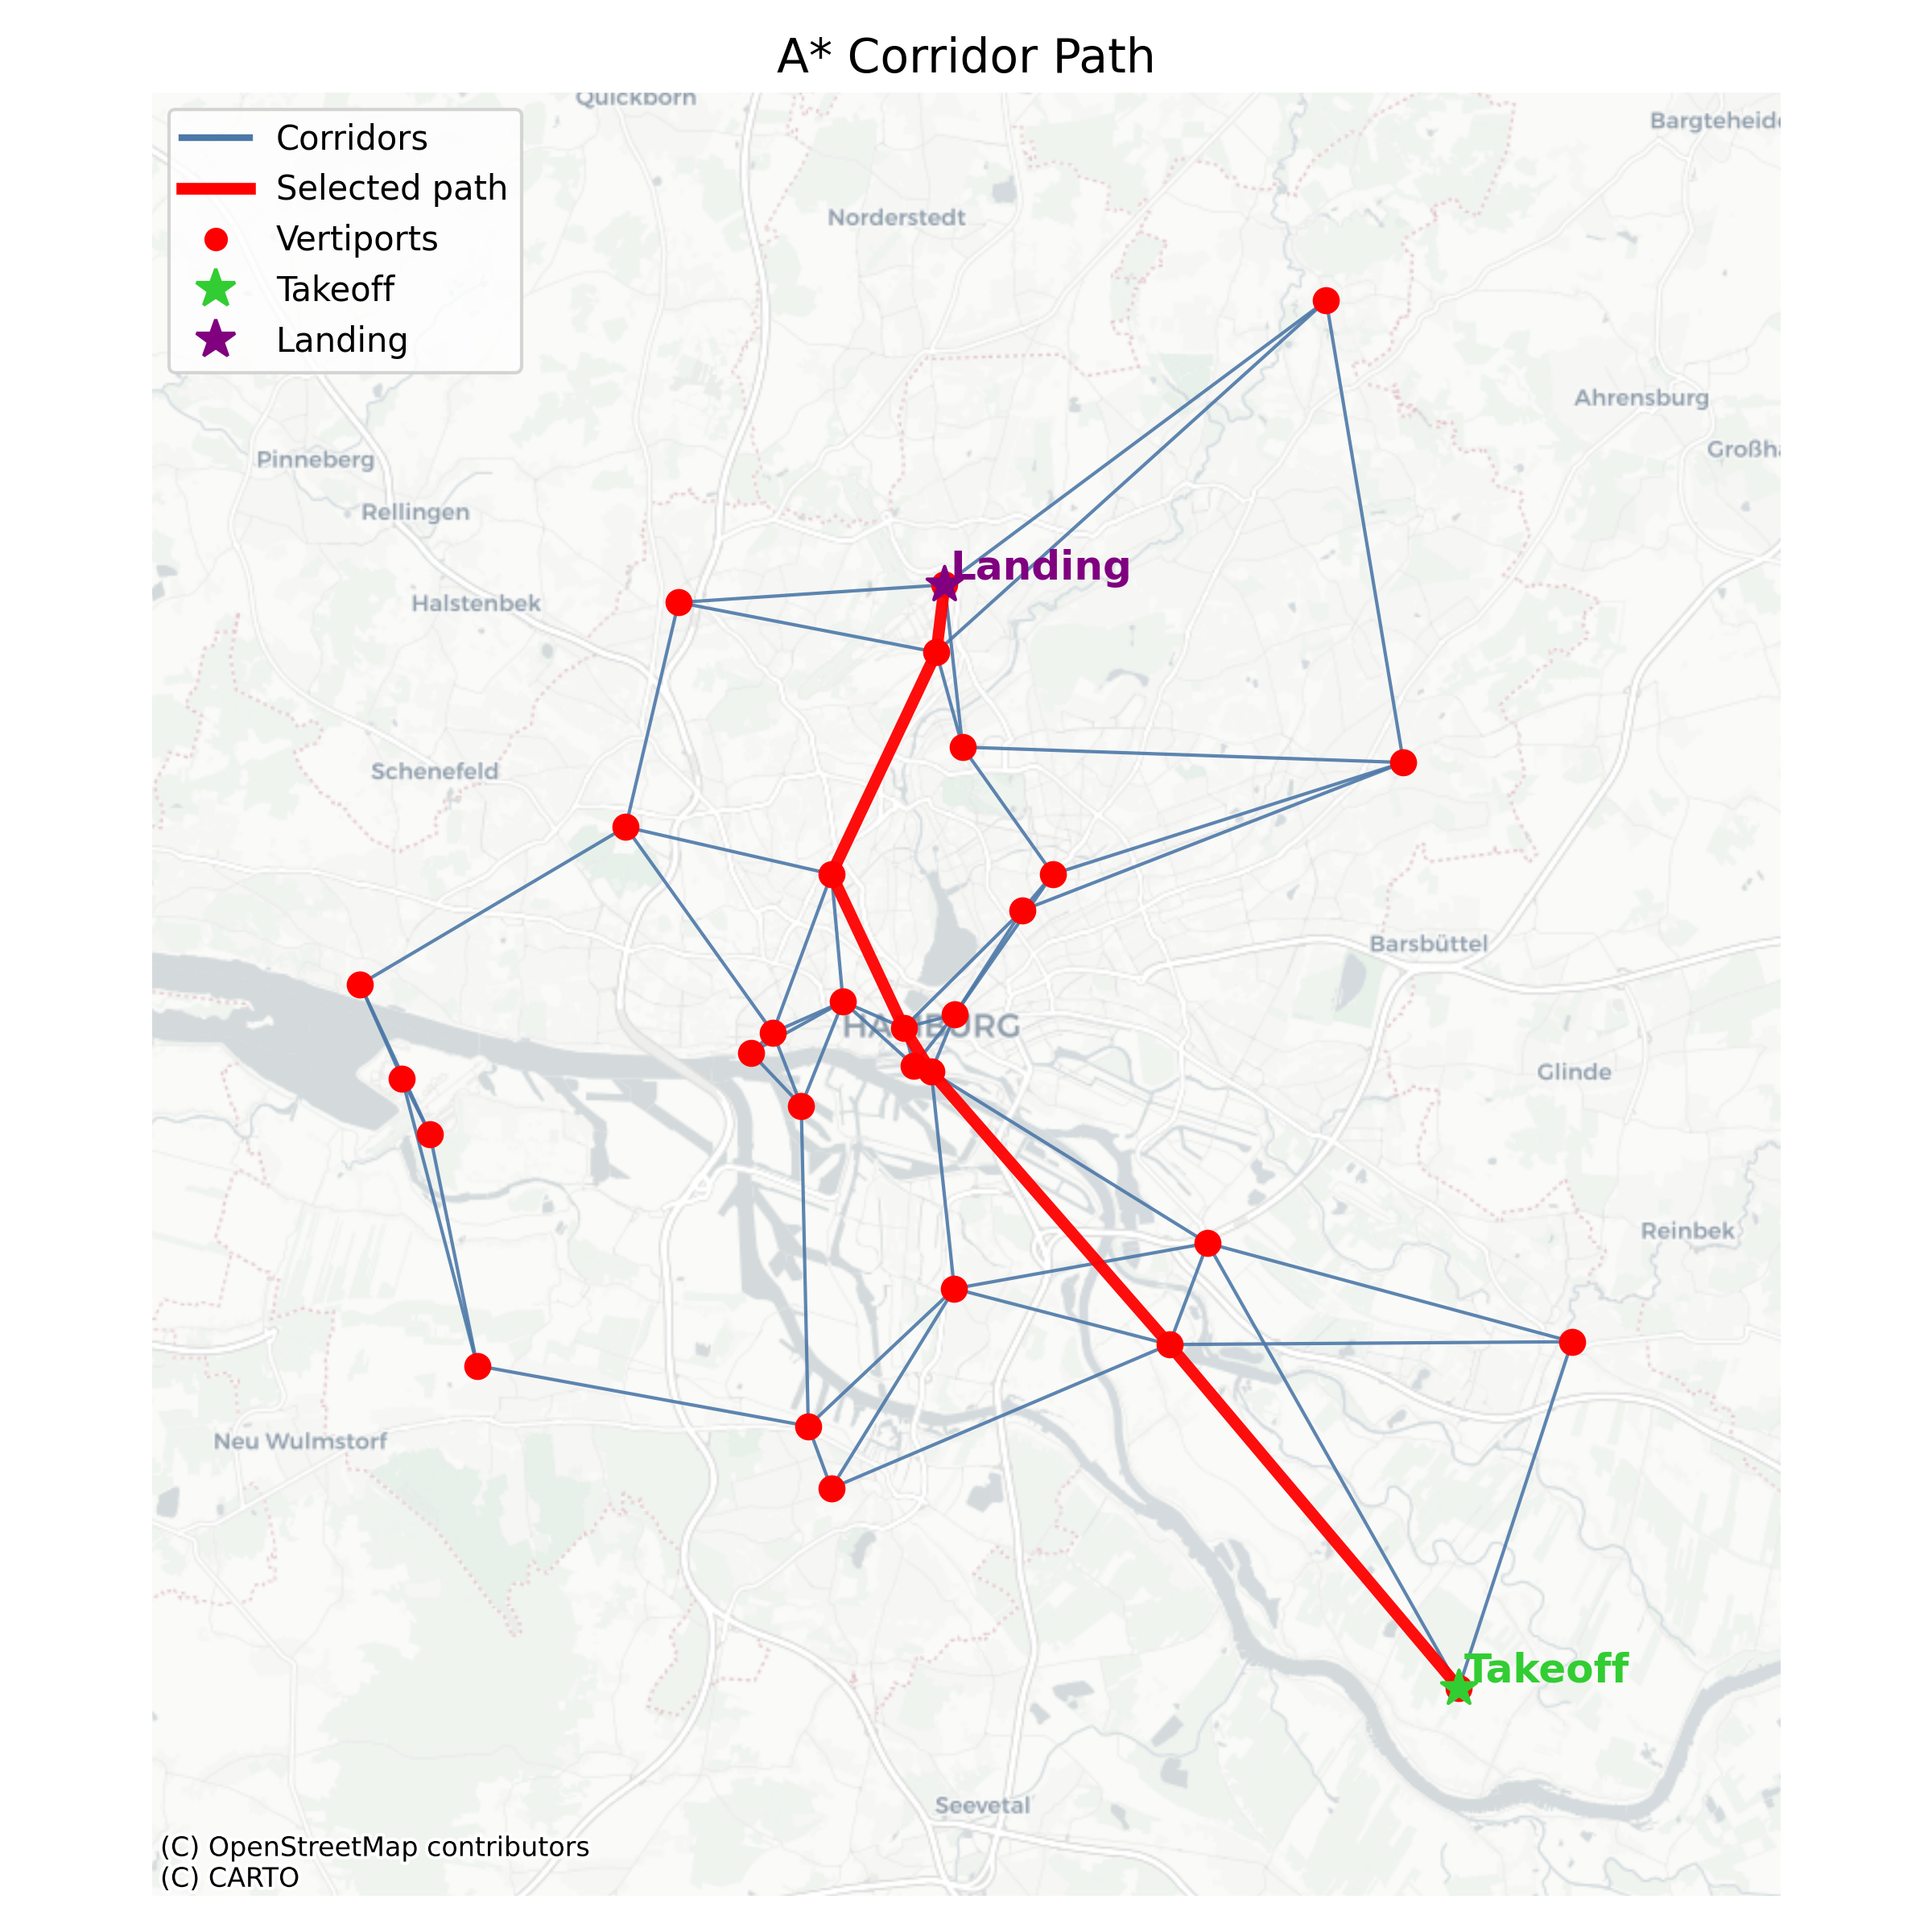
\includegraphics[width=0.6\textwidth]{results/trajectoryA_map.png}
  \caption{Planned reference trajectory (Trajectory A) from \(s\) to \(d\) over the Hamburg corridor network.}
  \label{fig:trajA_map}
\end{figure}

\subsubsection*{Front-end Visualization (Cesium)}
Figure~\ref{fig:trajA_cesium} shows the planned Trajectory~A rendered in the Cesium-based web client. 
The left view displays the full 3D corridor context of the route, while the right view 
zooms in on the departure phase to highlight the take-off and initial climb segment.

\begin{figure}[H]
  \centering
  \begin{subfigure}[t]{0.48\textwidth}
    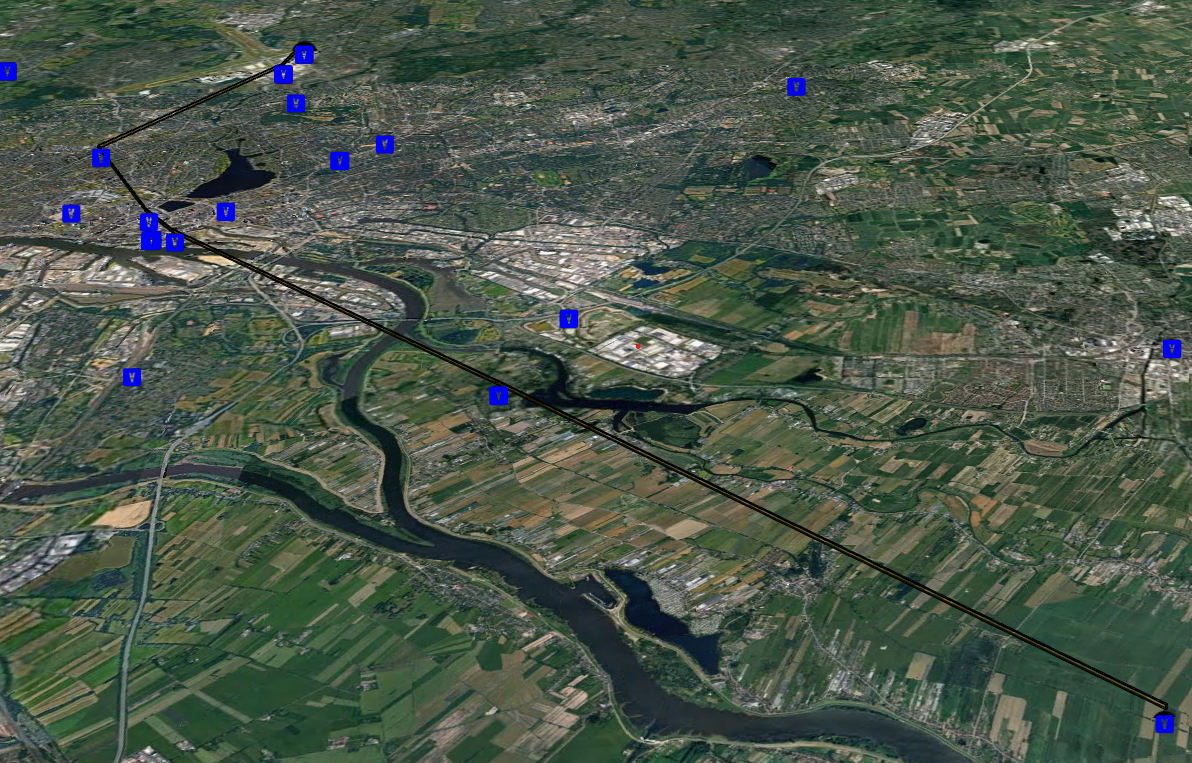
\includegraphics[width=\textwidth]{results/trajectoryA_cesium_full.png}
    \caption{Planned route (Trajectory A): full 3D corridor context.}
  \end{subfigure}
  \hfill
  \begin{subfigure}[t]{0.48\textwidth}
    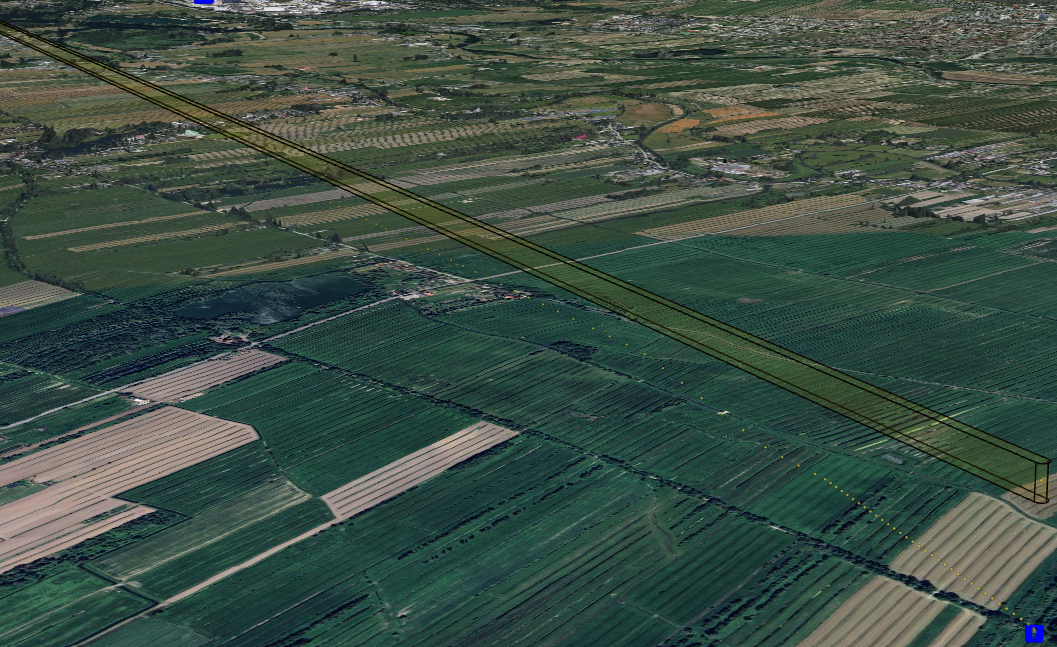
\includegraphics[width=\textwidth]{results/trajectoryA_cesium_takeoff.png}
    \caption{Planned route (Trajectory A): zoom on take-off and initial climb.}
  \end{subfigure}
  \caption{Cesium-based visualization of the planned Trajectory~A in the front end. Left: full route; right: take-off segment.}
  \label{fig:trajA_cesium}
\end{figure}

\subsubsection*{Kinematic Profiles}
\begin{figure}[H]
  \centering
  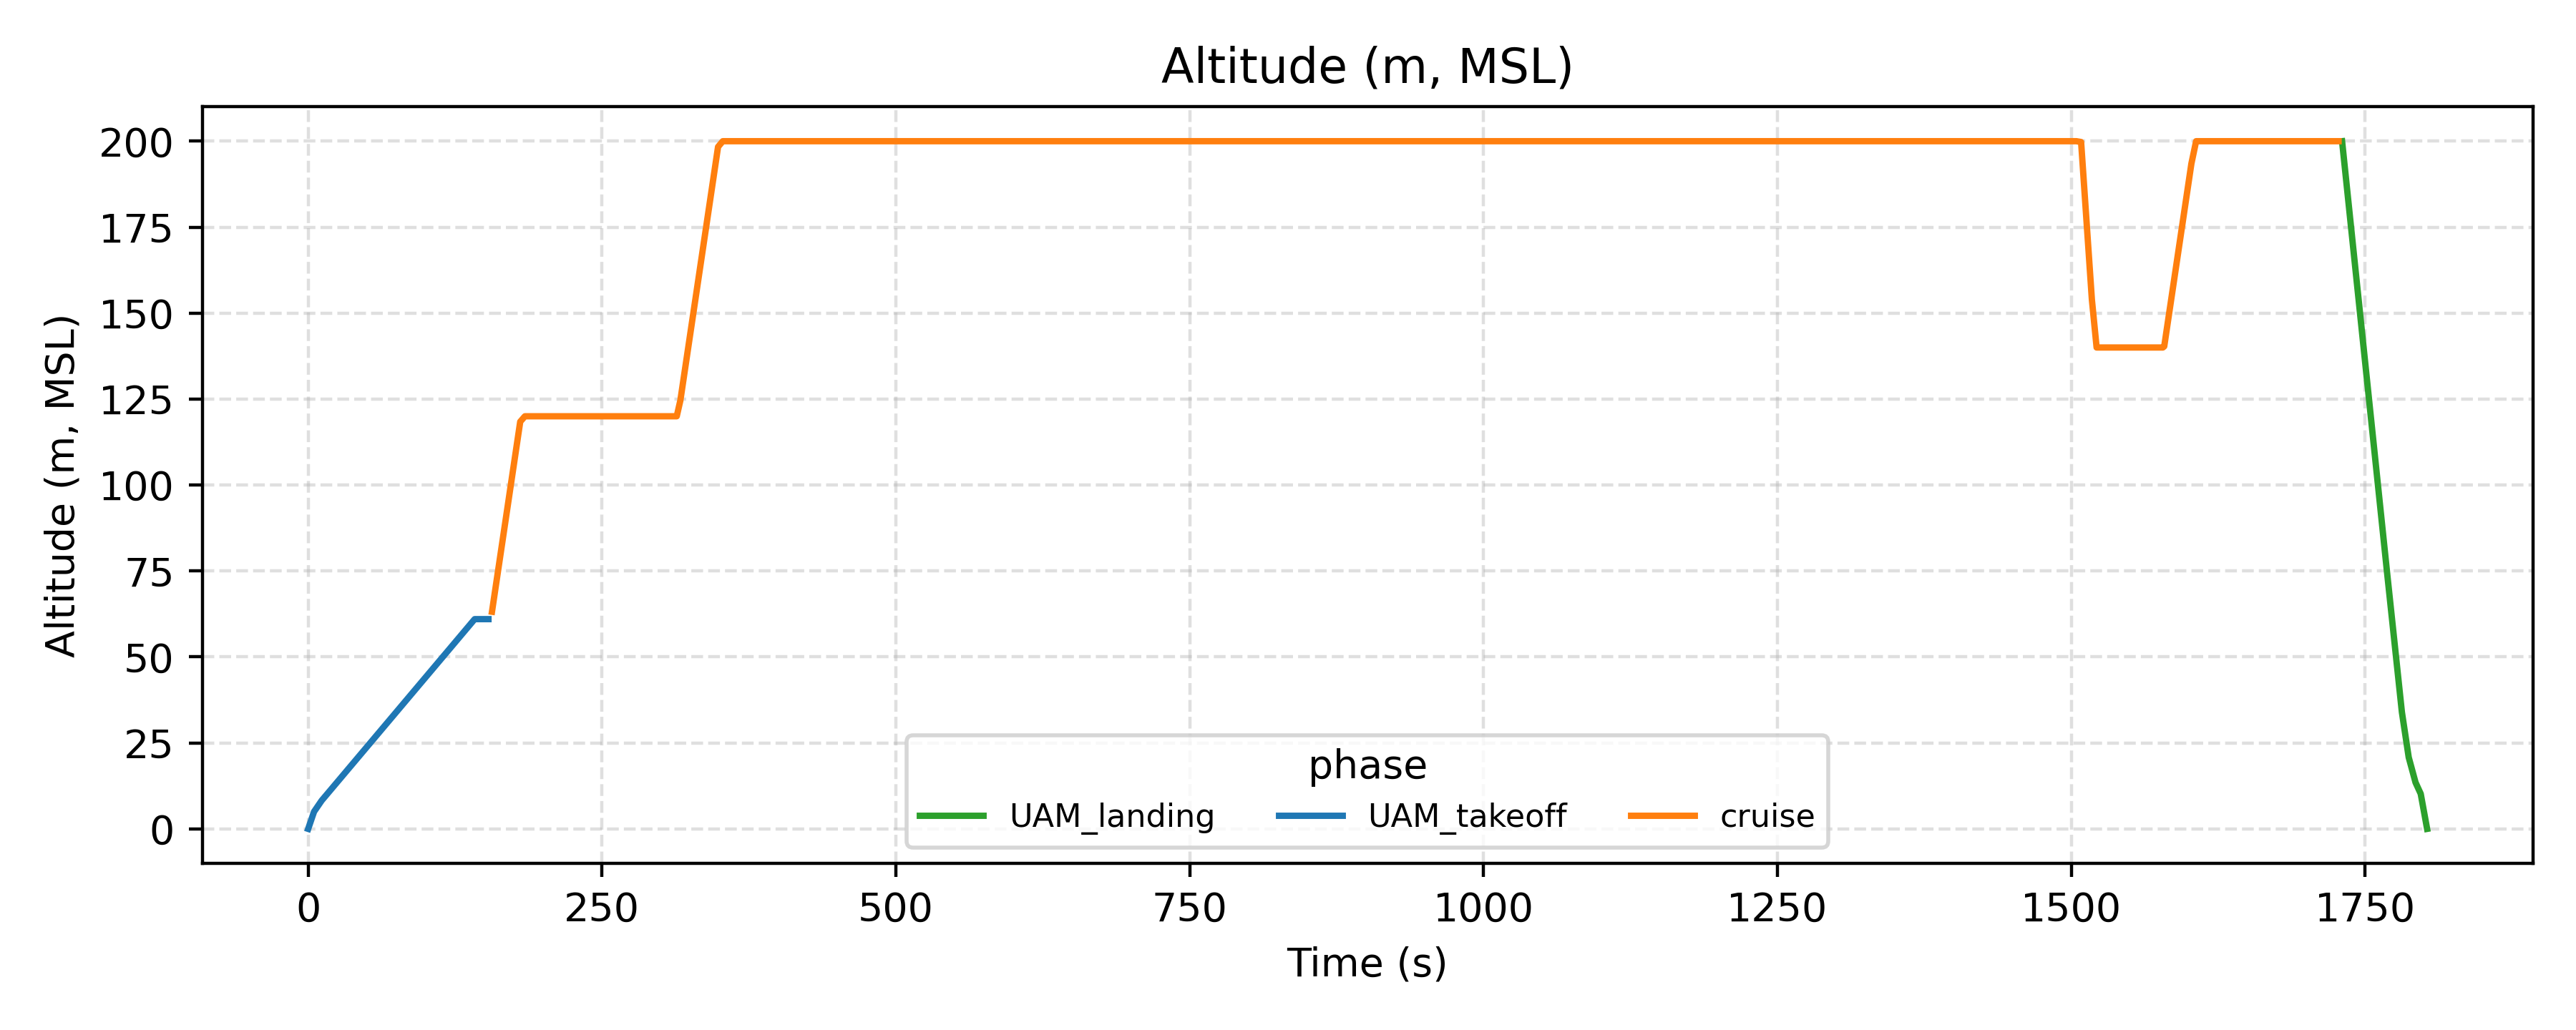
\includegraphics[width=0.86\textwidth]{results/trajectoryA_altitude.png}
  \caption{Planned altitude profile \(H(\tau)\) for Trajectory A (cruise layer near \SI{200}{m} AGL).}
  \label{fig:trajA_alt}
\end{figure}

\begin{figure}[H]
  \centering
  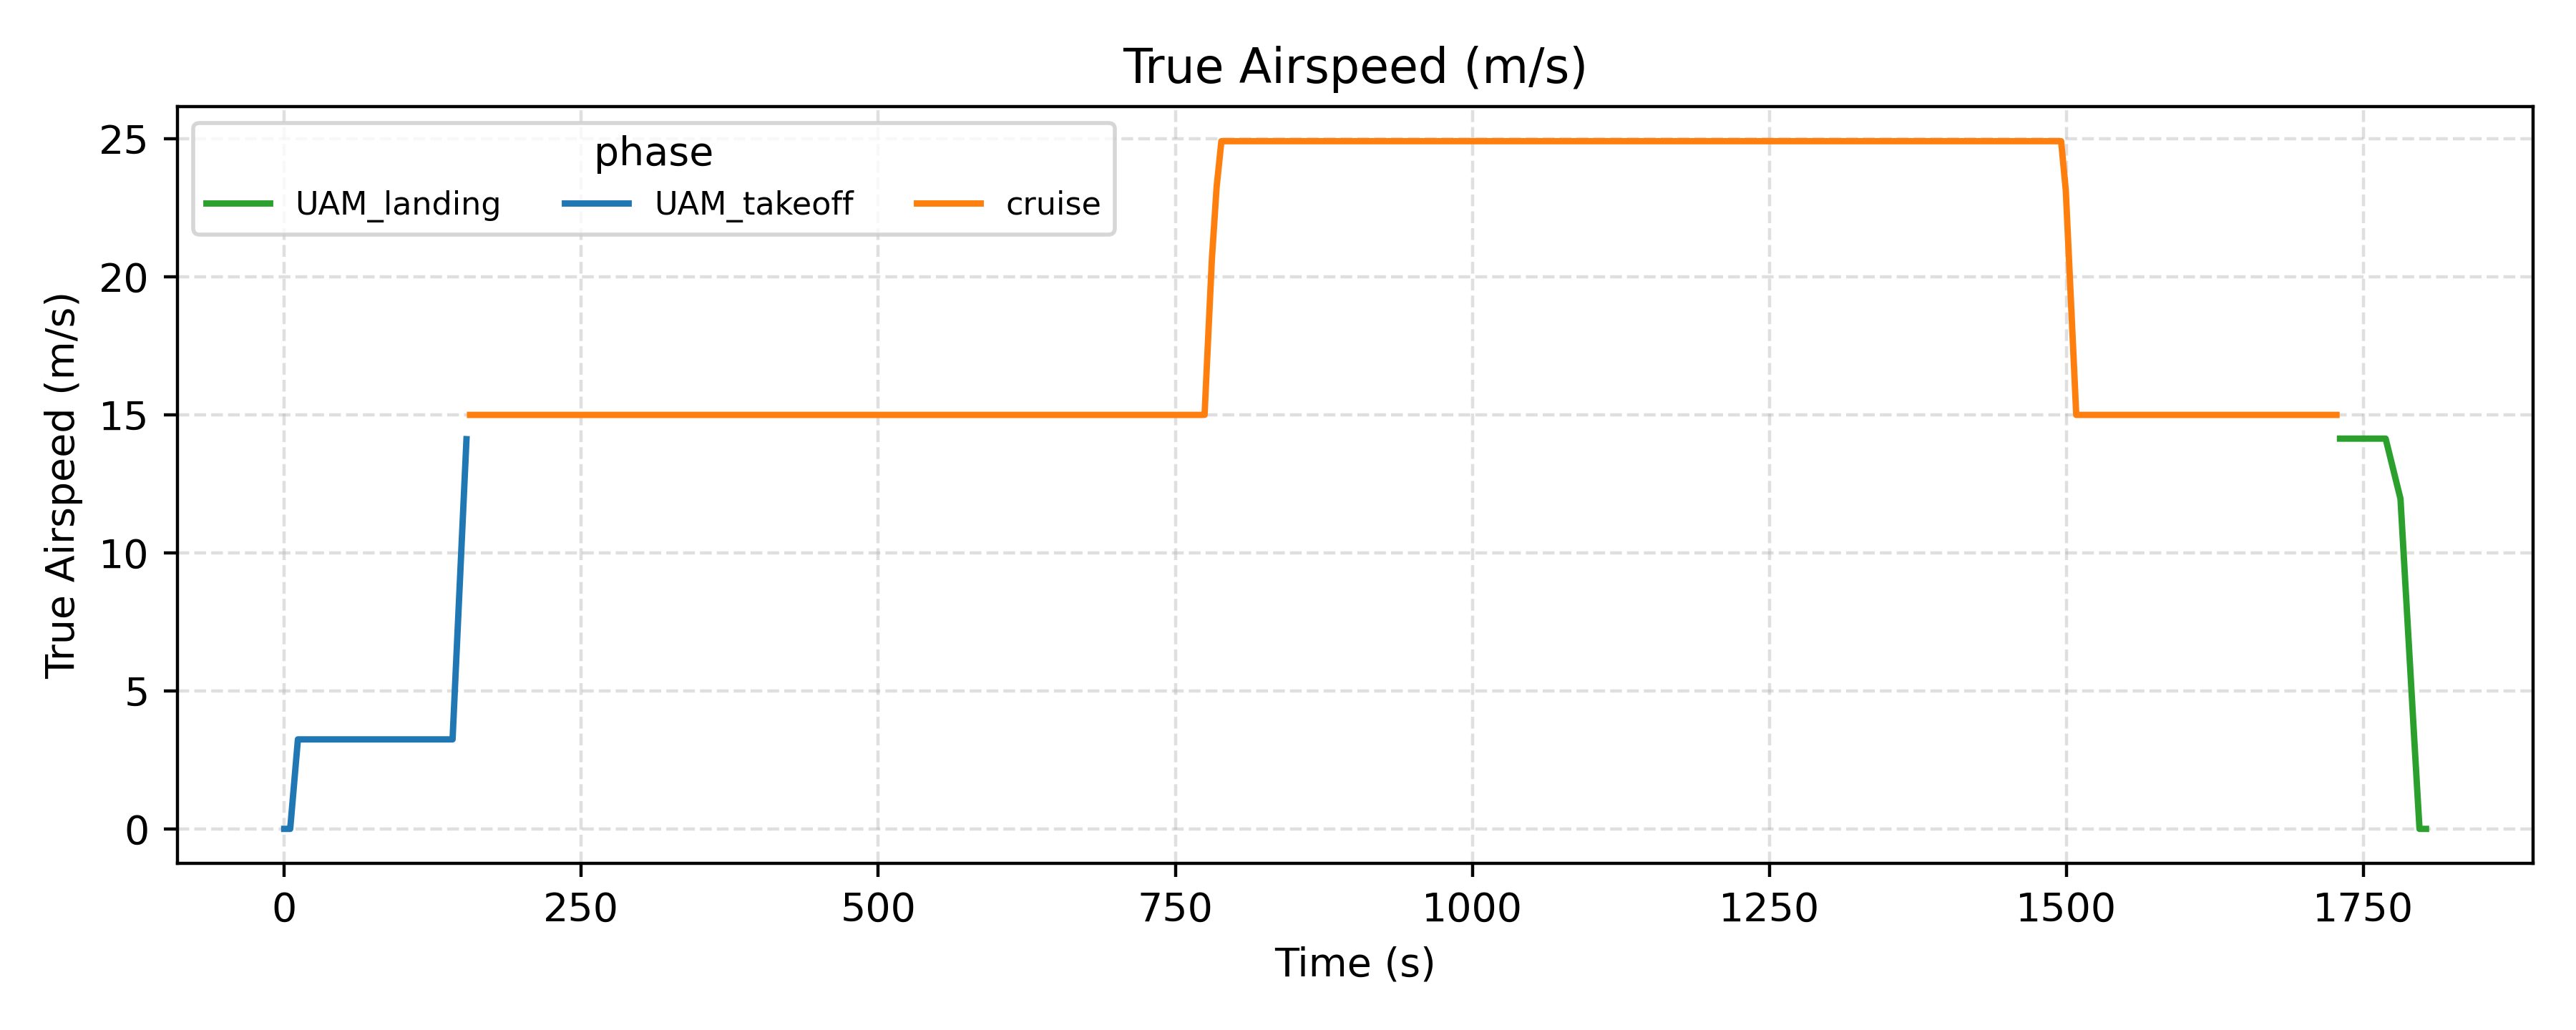
\includegraphics[width=0.86\textwidth]{results/trajectoryA_TAS.png}
  \caption{Planned true airspeed (TAS) profile for Trajectory A.}
  \label{fig:trajA_tas}
\end{figure}

\begin{figure}[H]
  \centering
  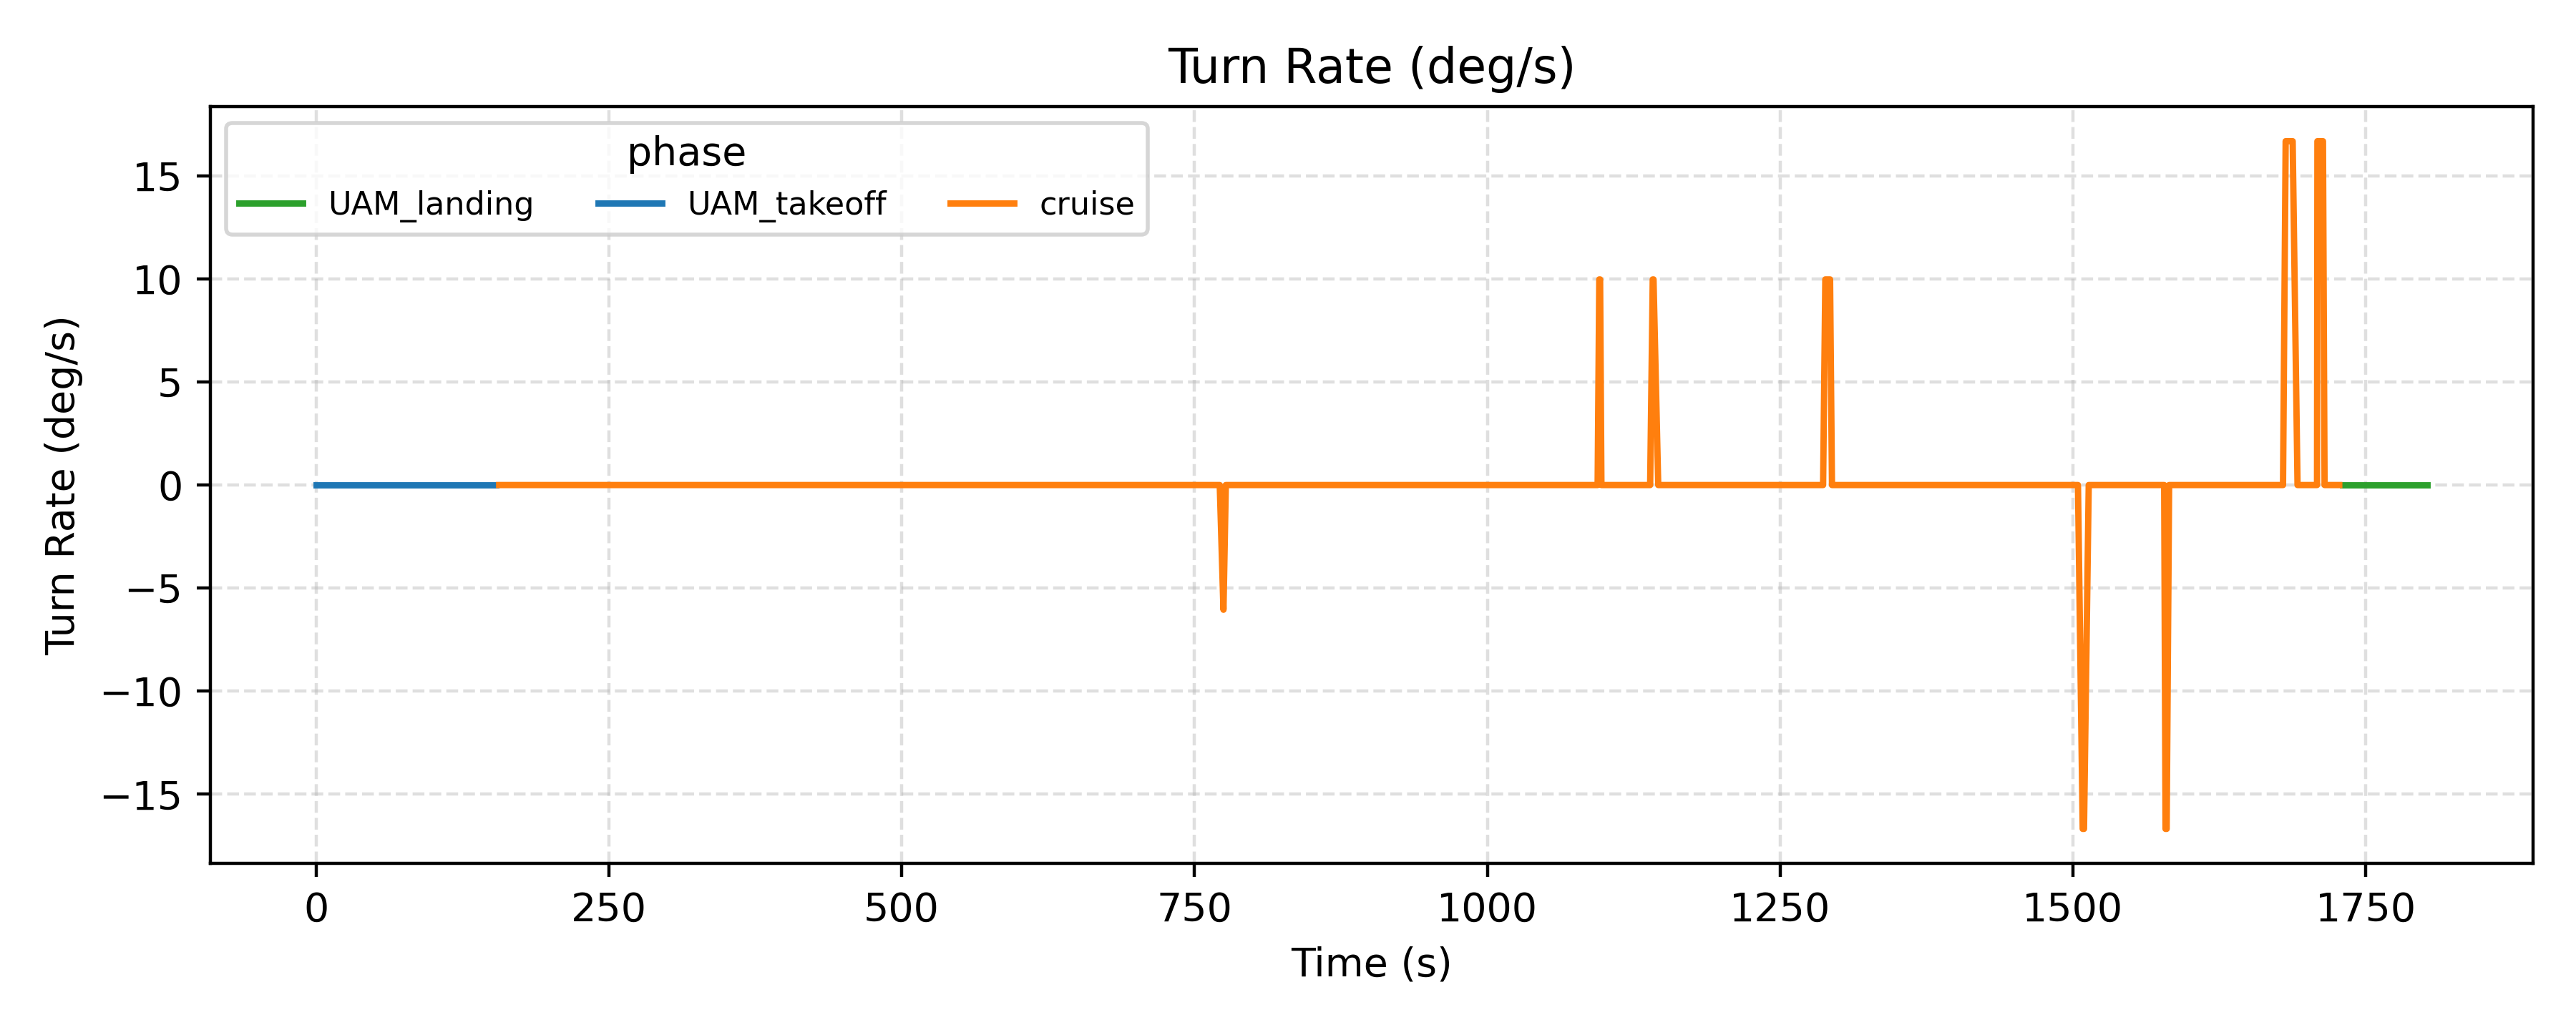
\includegraphics[width=0.86\textwidth]{results/trajectoryA_turn.png}
  \caption{Planned turn-rate profile \(\dot{\psi}(\tau)\) for Trajectory A (deg/s).}
  \label{fig:trajA_turn}
\end{figure}

\begin{figure}[H]
  \centering
  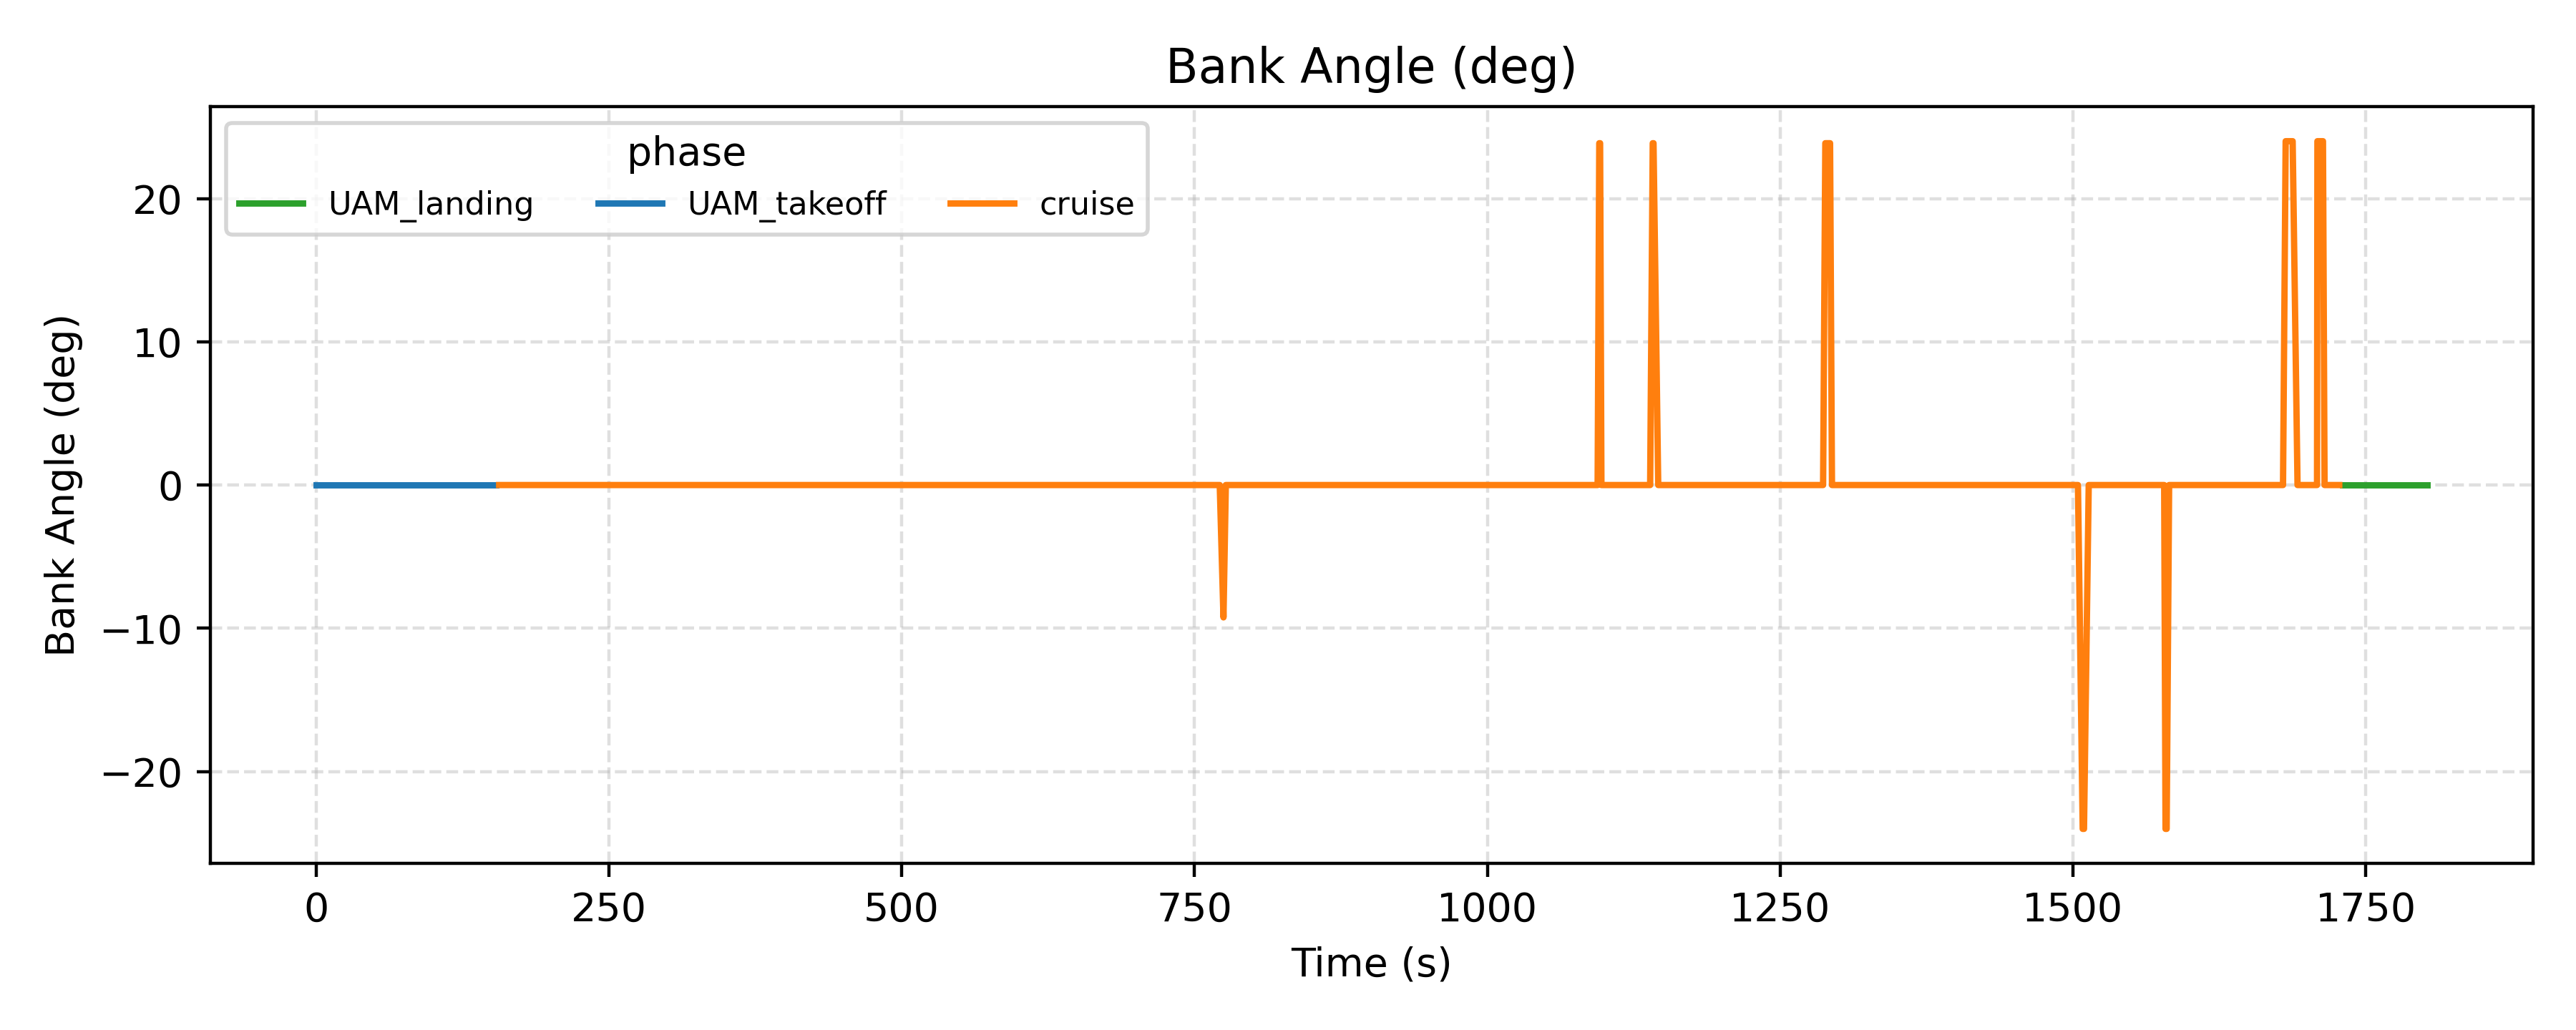
\includegraphics[width=0.86\textwidth]{results/trajectoryA_bank.png}
  \caption{Planned bank-angle profile $\phi(\tau)$ for Trajectory A (deg).}
  \label{fig:trajA_bank}
\end{figure}

\paragraph{Interpretation of bank angle and turn-rate profiles (CFMS).}
At each turn waypoint, the inbound and outbound ground tracks define the required course change \(\Delta\chi\) and the turn direction. 
CFMS then synthesizes a dynamically feasible turn using the aircraft performance limits (maximum load factor and bank-rate limit) at the current \emph{groundspeed} \(V_g\) (speed over ground, i.e., the magnitude of the ground-relative velocity vector) \cite{morscheck2021cfms}. 
The constructed turn has three phases: bank-up, constant-bank arc, and bank-down. A bank-rate bound \(\dot\phi_{\max}\) shapes the transients; if the transients would exceed the geometric corner, CFMS reduces the allowable bank to fit the fillet.

The bank ceiling is set by the maximum load factor \(n_{\max}\) under coordinated-turn assumptions:
\begin{equation}
  \phi_{\max} \;=\; \arccos\!\left(\frac{1}{n_{\max}}\right).
\end{equation}
The instantaneous turn rate follows coordinated-turn kinematics:
\begin{equation}
  \dot\psi(t) \;=\; \frac{g\,\tan\!\big(\phi(t)\big)}{V_g(t)}\,,
\end{equation}
so, for a given \(V_g\), the largest achievable turn rate is
\begin{equation}
  \dot\psi_{\max} \;=\; \frac{g\,\tan(\phi_{\max})}{V_g}\,.
\end{equation}

\noindent\textit{Consistency check for reported peaks.}
Using the study’s typical value \(n_{\max}=1.1\) (small UAS),
\begin{equation}
  \phi_{\max} \;\approx\; \arccos\!\left(\frac{1}{1.1}\right) \;\approx\; 24.6^{\circ},
\end{equation}
which is consistent with the observed \(\max \phi \approx 24.0^{\circ}\).
At a representative transitional groundspeed \(V_g \approx 15~\mathrm{m/s}\),
\begin{equation}
    \begin{aligned}
      \dot\psi_{\max} 
      &\;\approx\; \frac{9.81\,\tan(24^{\circ})}{15}\;\; \mathrm{rad/s} \\
      &\;\approx\; 0.29~\mathrm{rad/s} \;\approx\; 16.7^{\circ}\!/\mathrm{s},
    \end{aligned}  
\end{equation}
matching the reported \(\max \dot\psi \approx 16.68^{\circ}\!/\mathrm{s}\).
(When CFMS’s simplified point-to-point routine is used, a capped constant turn rate may be applied instead of the full filleted turn.)

\subsubsection*{Summary Statistics}
\begin{table}[H]
  \centering
  \caption{Summary statistics for the planned reference Trajectory A.}
  \label{tab:trajA_summary}
  \begin{tabular}{l r}
    \toprule
    Points & \num{500} \\
    Total time $T$ (s) & \num{1802.71} \\
    Total time $T$ (min) & \num{30.05} \\
    Total distance $L$ (km) & \num{32.13} \\
    Mean TAS (m/s) & \num{17.88} \\
    Peak bank angle $\max \phi$ (deg) & \num{24.01} \\
    Peak turn rate $\max \dot{\psi}$ (deg/s) & \num{16.68} \\
    Peak climb rate $\max \dot{H}$ (m/s) & \num{6.10} \\
    \bottomrule
  \end{tabular}
\end{table}

\subsection{Representative Short-Leg Route}
\label{sec:trajB}

Trajectory B was chosen to illustrate the behavior of the system when the initial leg is relatively short. 
In this case, the UAM vehicle has limited horizontal distance available during the first segment, 
requiring it to execute a circular turning maneuver in order to gain sufficient altitude 
and align with the required waypoint. 
This scenario highlights the interaction between climb dynamics and network geometry, 
making it a complementary test case to Trajectory A.

\subsubsection*{Route Overview}
\begin{figure}[H]
  \centering
  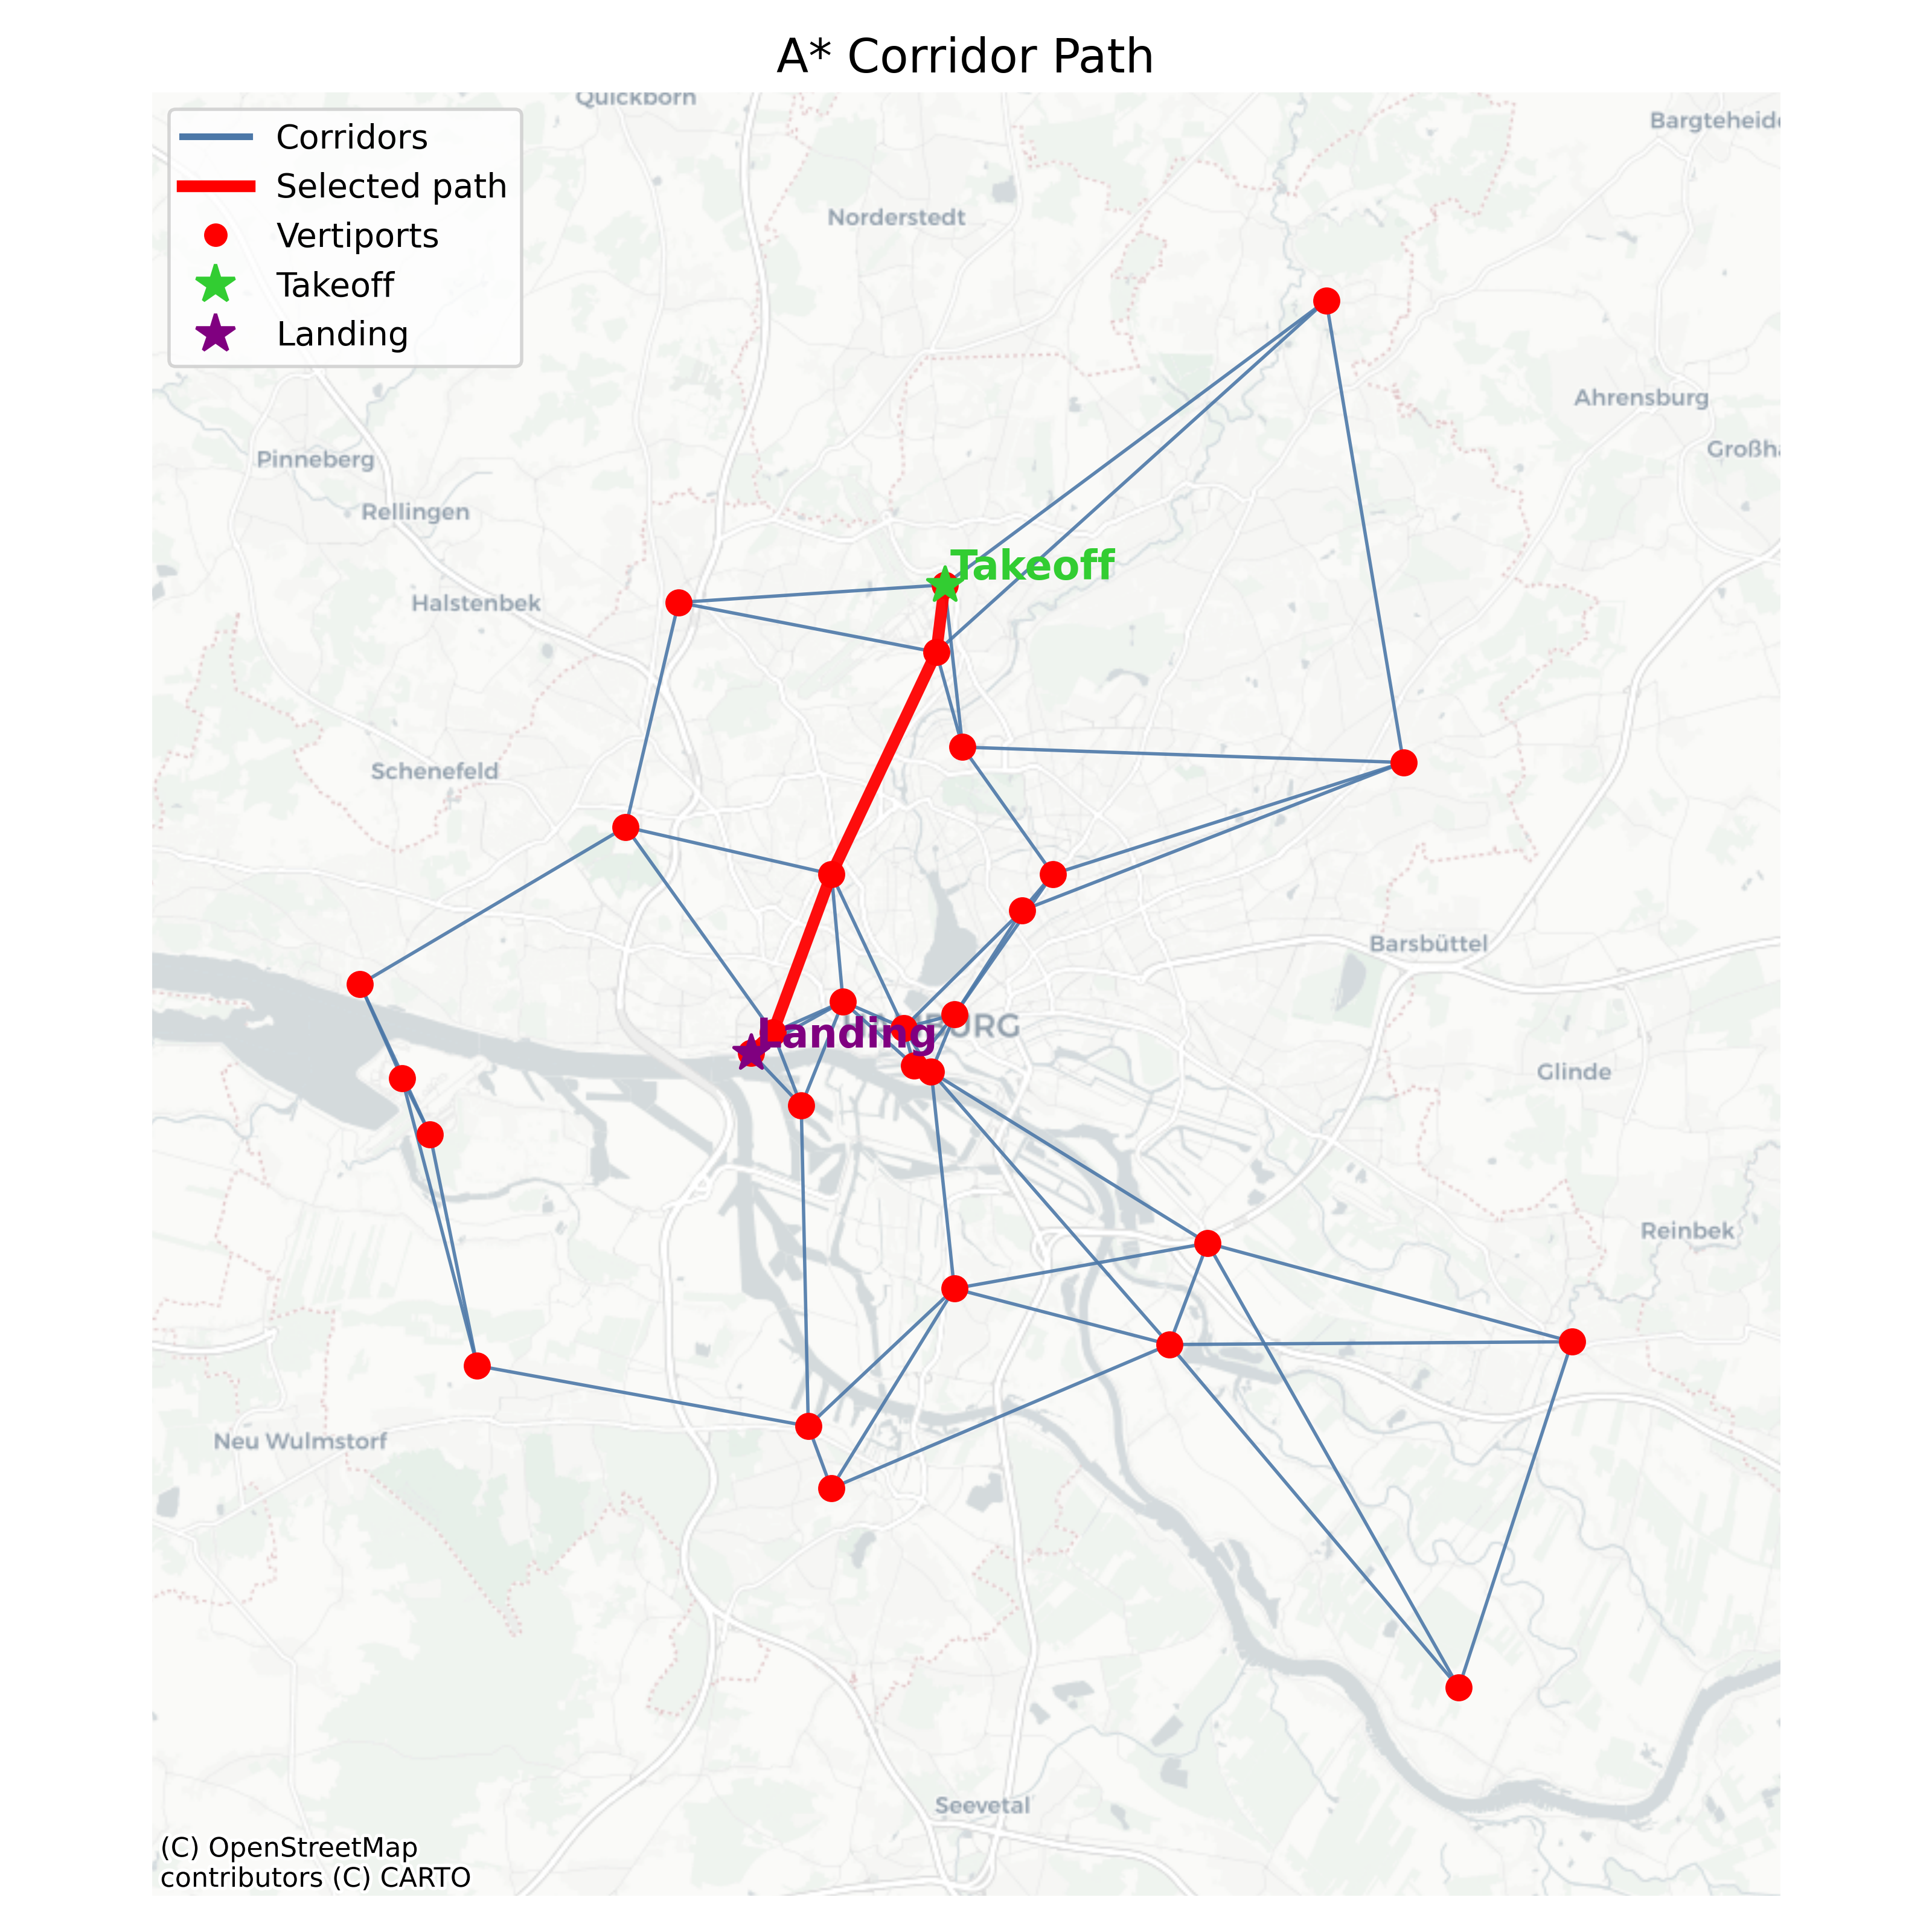
\includegraphics[width=0.5\textwidth]{results/trajectoryB_map.png}
  \caption{Planned reference trajectory (Trajectory B) from \(s\) to \(d\) over the Hamburg corridor network.}
  \label{fig:trajB_map}
\end{figure}

\subsubsection*{Front-end Visualization (Cesium)}
Figure~\ref{fig:trajB_cesium} shows the planned Trajectory~B in the Cesium-based front end. 
The left panel displays the full 3D route, while the right panel zooms into 
the departure phase, illustrating the short initial leg and the early turning manoeuvre 
required to reach the first waypoint.

\begin{figure}[H]
  \centering
  \begin{subfigure}[t]{0.48\textwidth}
    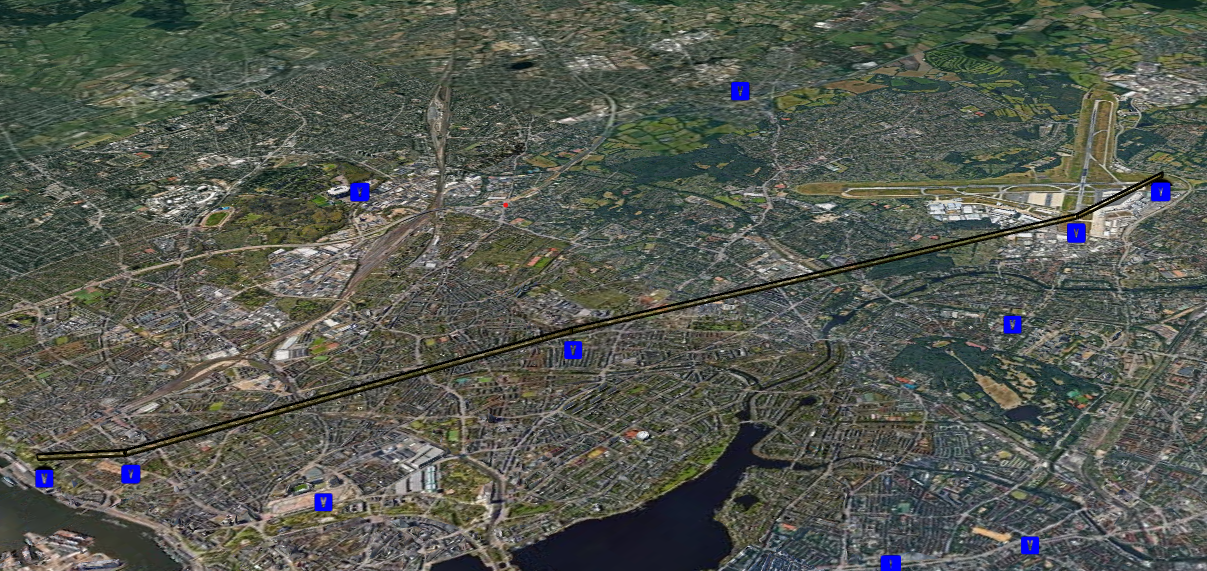
\includegraphics[width=\textwidth]{results/trajectoryB_cesium_full.png}
    \caption{Planned route (Trajectory B): full 3D corridor context.}
  \end{subfigure}
  \hfill
  \begin{subfigure}[t]{0.48\textwidth}
    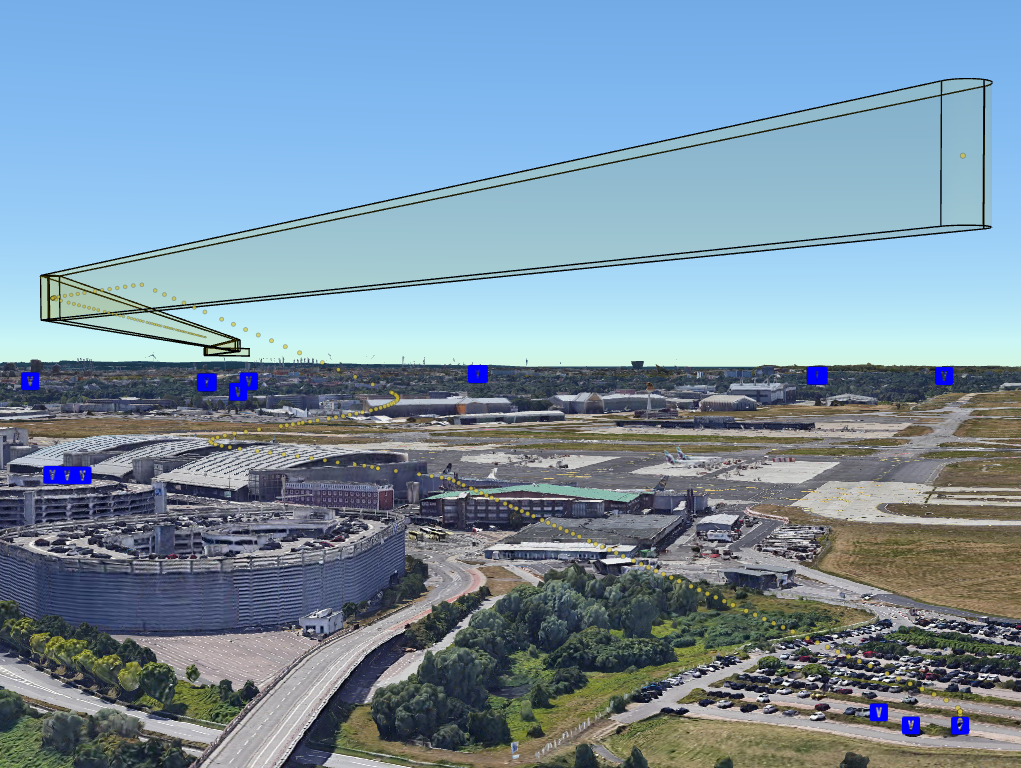
\includegraphics[width=\textwidth]{results/trajectoryB_cesium_takeoff.png}
    \caption{Planned route (Trajectory B): zoom on take-off and initial turning manoeuvre.}
  \end{subfigure}
  \caption{Cesium-based visualization of the planned Trajectory~B in the front end. Left: full route; right: take-off segment.}
  \label{fig:trajB_cesium}
\end{figure}

\subsubsection*{Kinematic Profiles}
\begin{figure}[H]
  \centering
  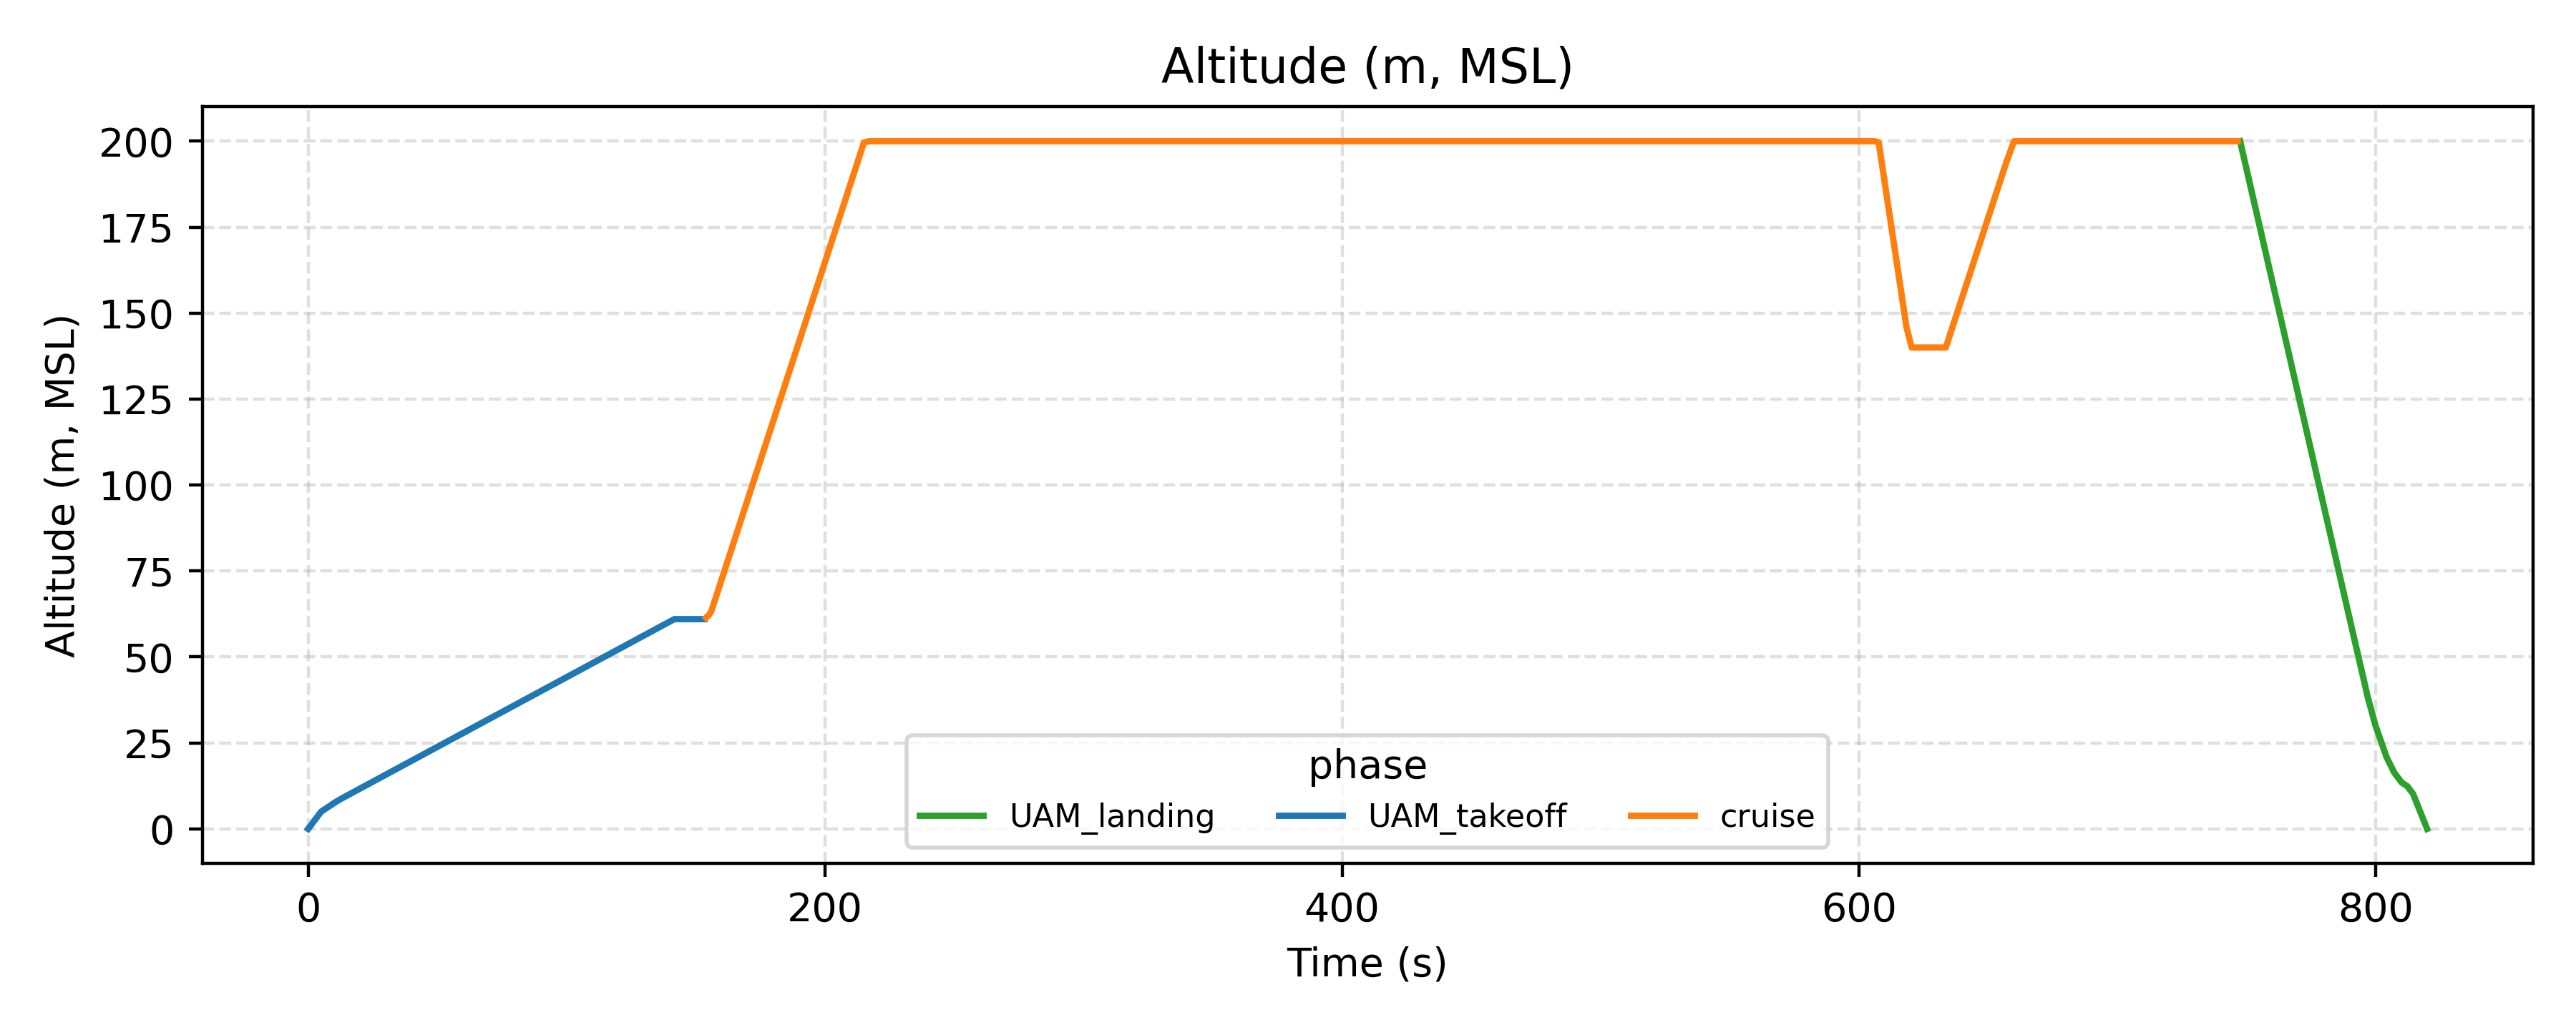
\includegraphics[width=0.86\textwidth]{results/trajectoryB_altitude.png}
  \caption{Planned altitude profile \(H(\tau)\) for Trajectory B (cruise layer near \SI{200}{m} AGL).}
  \label{fig:trajB_alt}
\end{figure}

\begin{figure}[H]
  \centering
  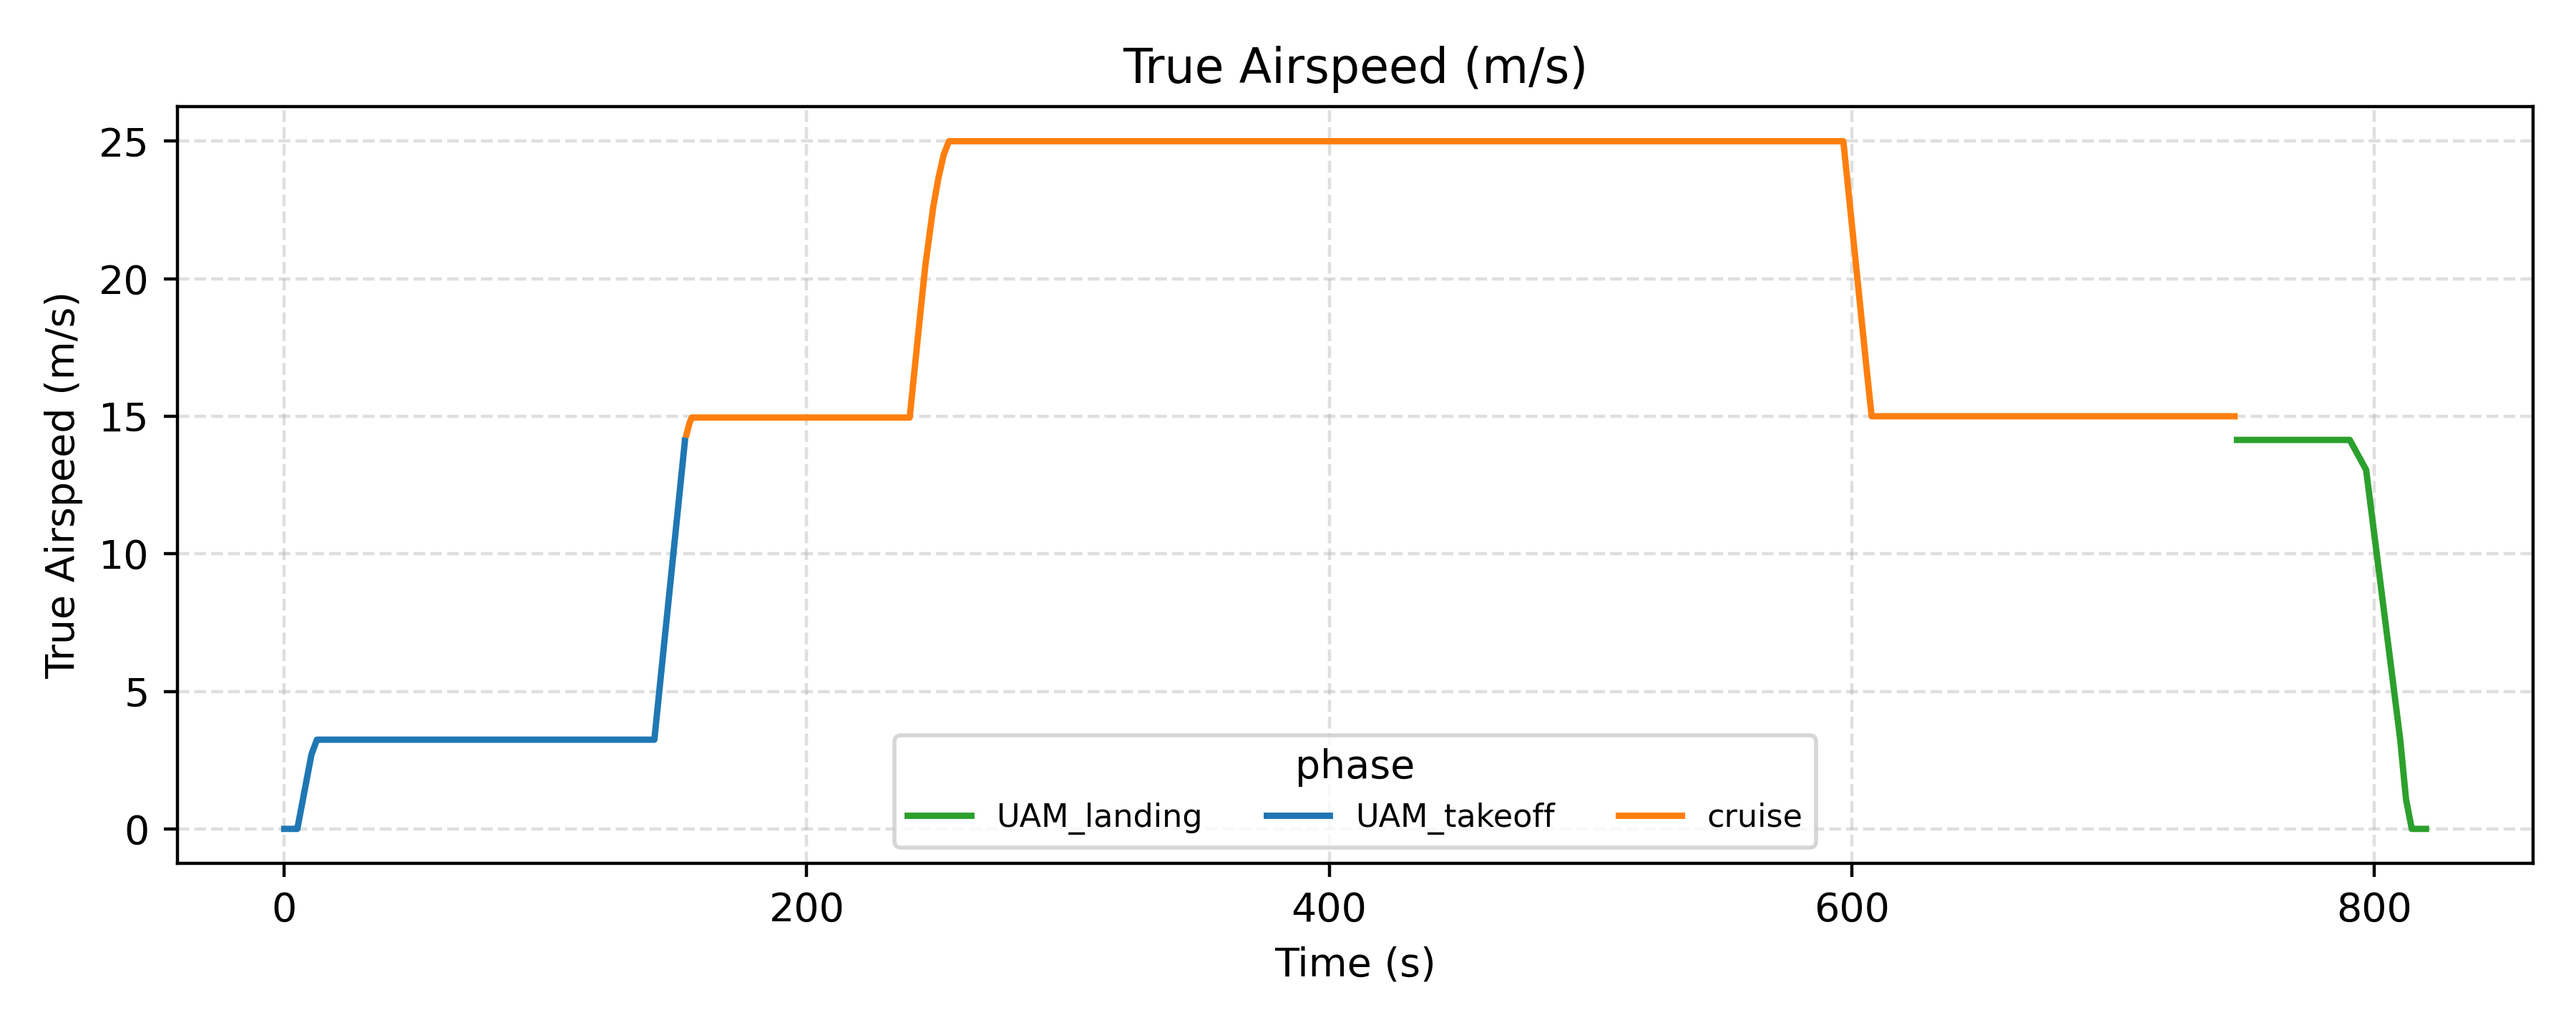
\includegraphics[width=0.86\textwidth]{results/trajectoryB_TAS.png}
  \caption{Planned true airspeed (TAS) profile for Trajectory B.}
  \label{fig:trajB_tas}
\end{figure}

\begin{figure}[H]
  \centering
  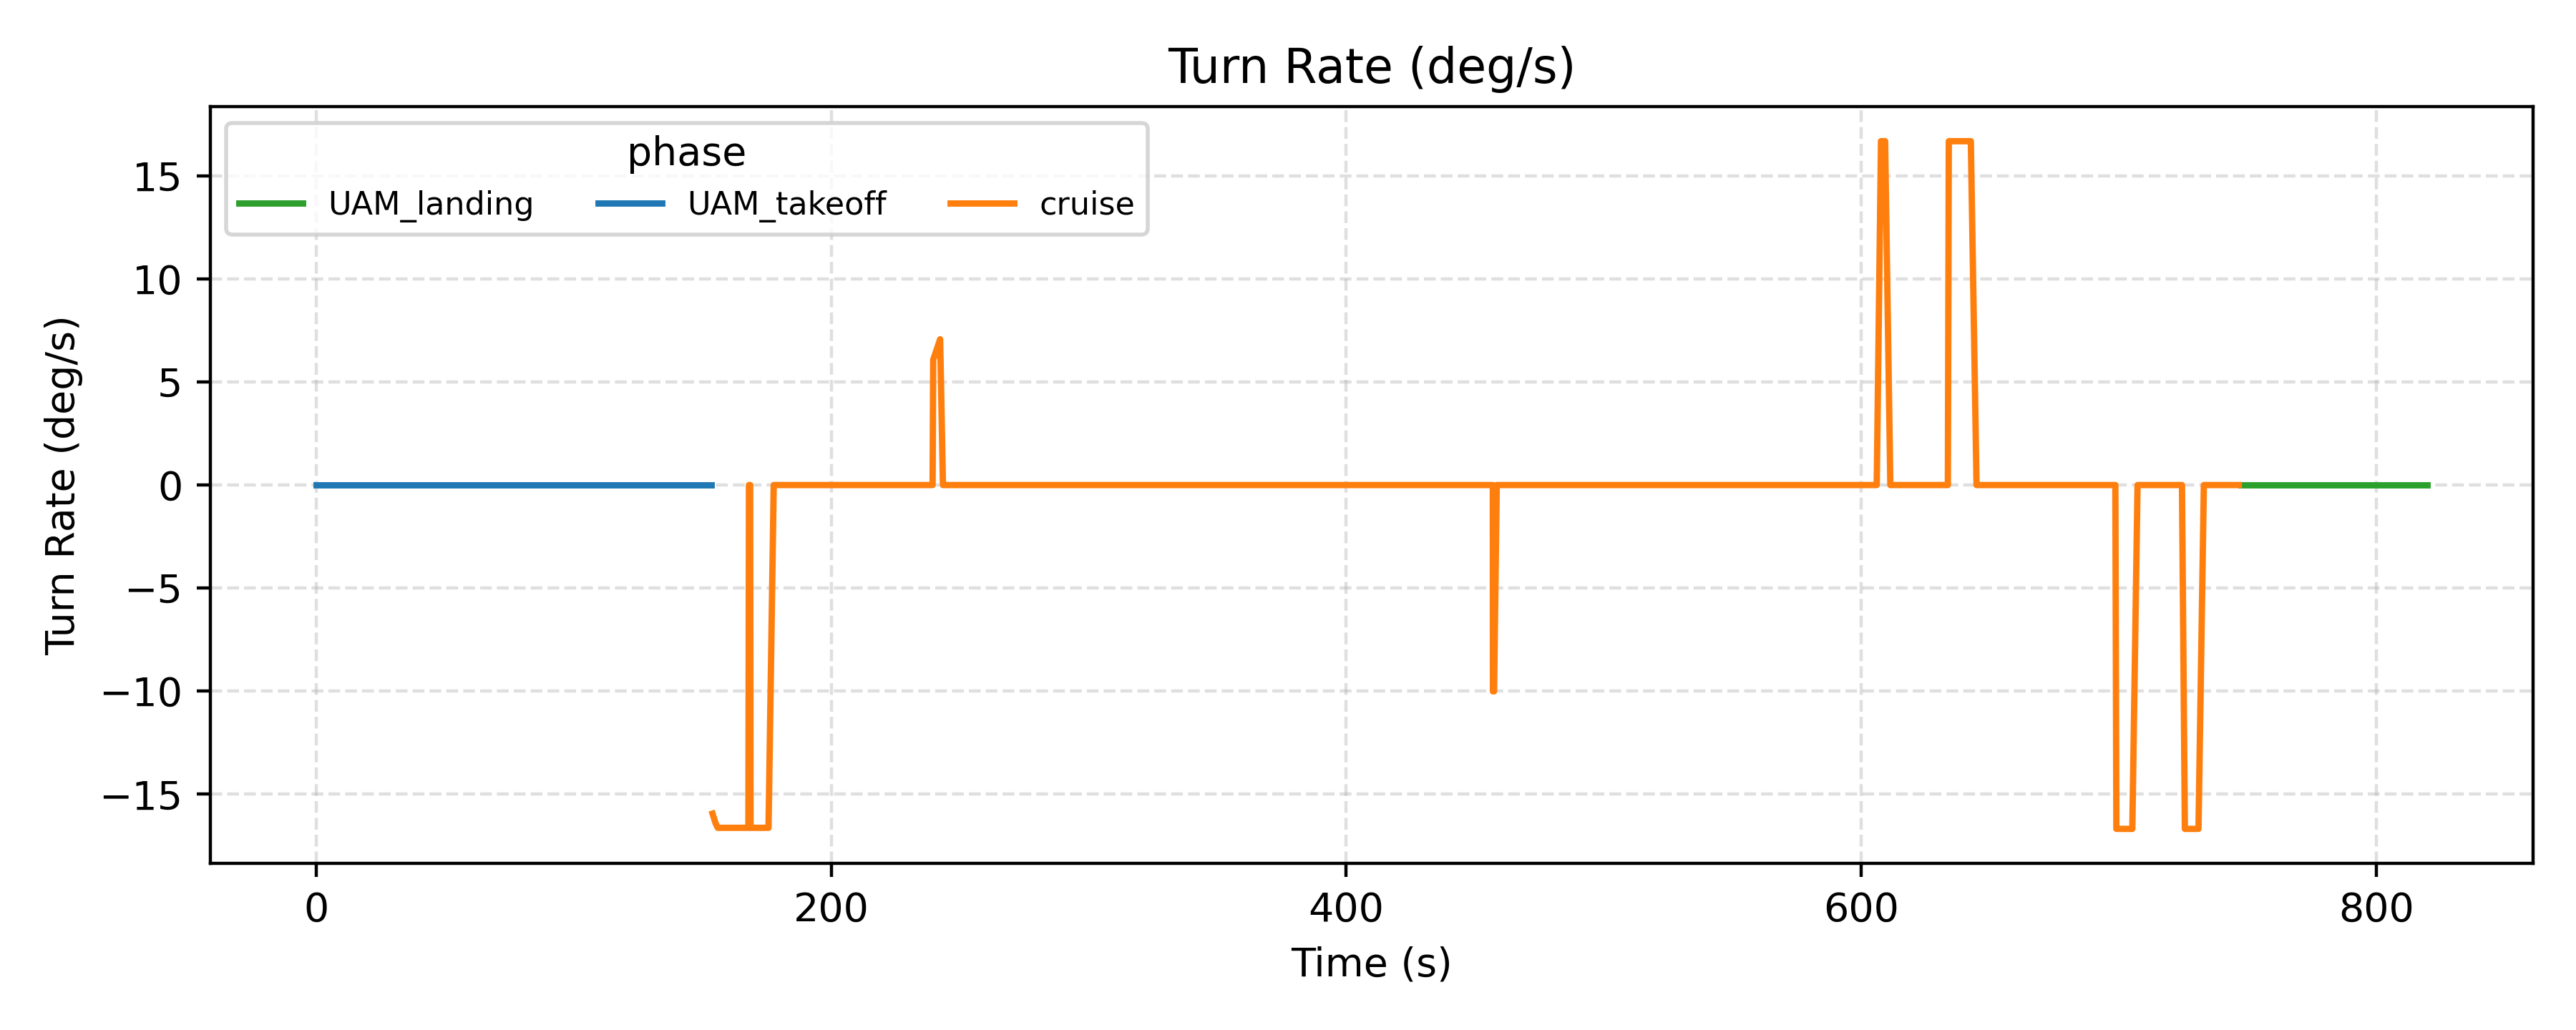
\includegraphics[width=0.86\textwidth]{results/trajectoryB_turn.png}
  \caption{Planned turn-rate profile \(\dot{\psi}(\tau)\) for Trajectory B (deg/s).}
  \label{fig:trajB_turn}
\end{figure}

\begin{figure}[H]
  \centering
  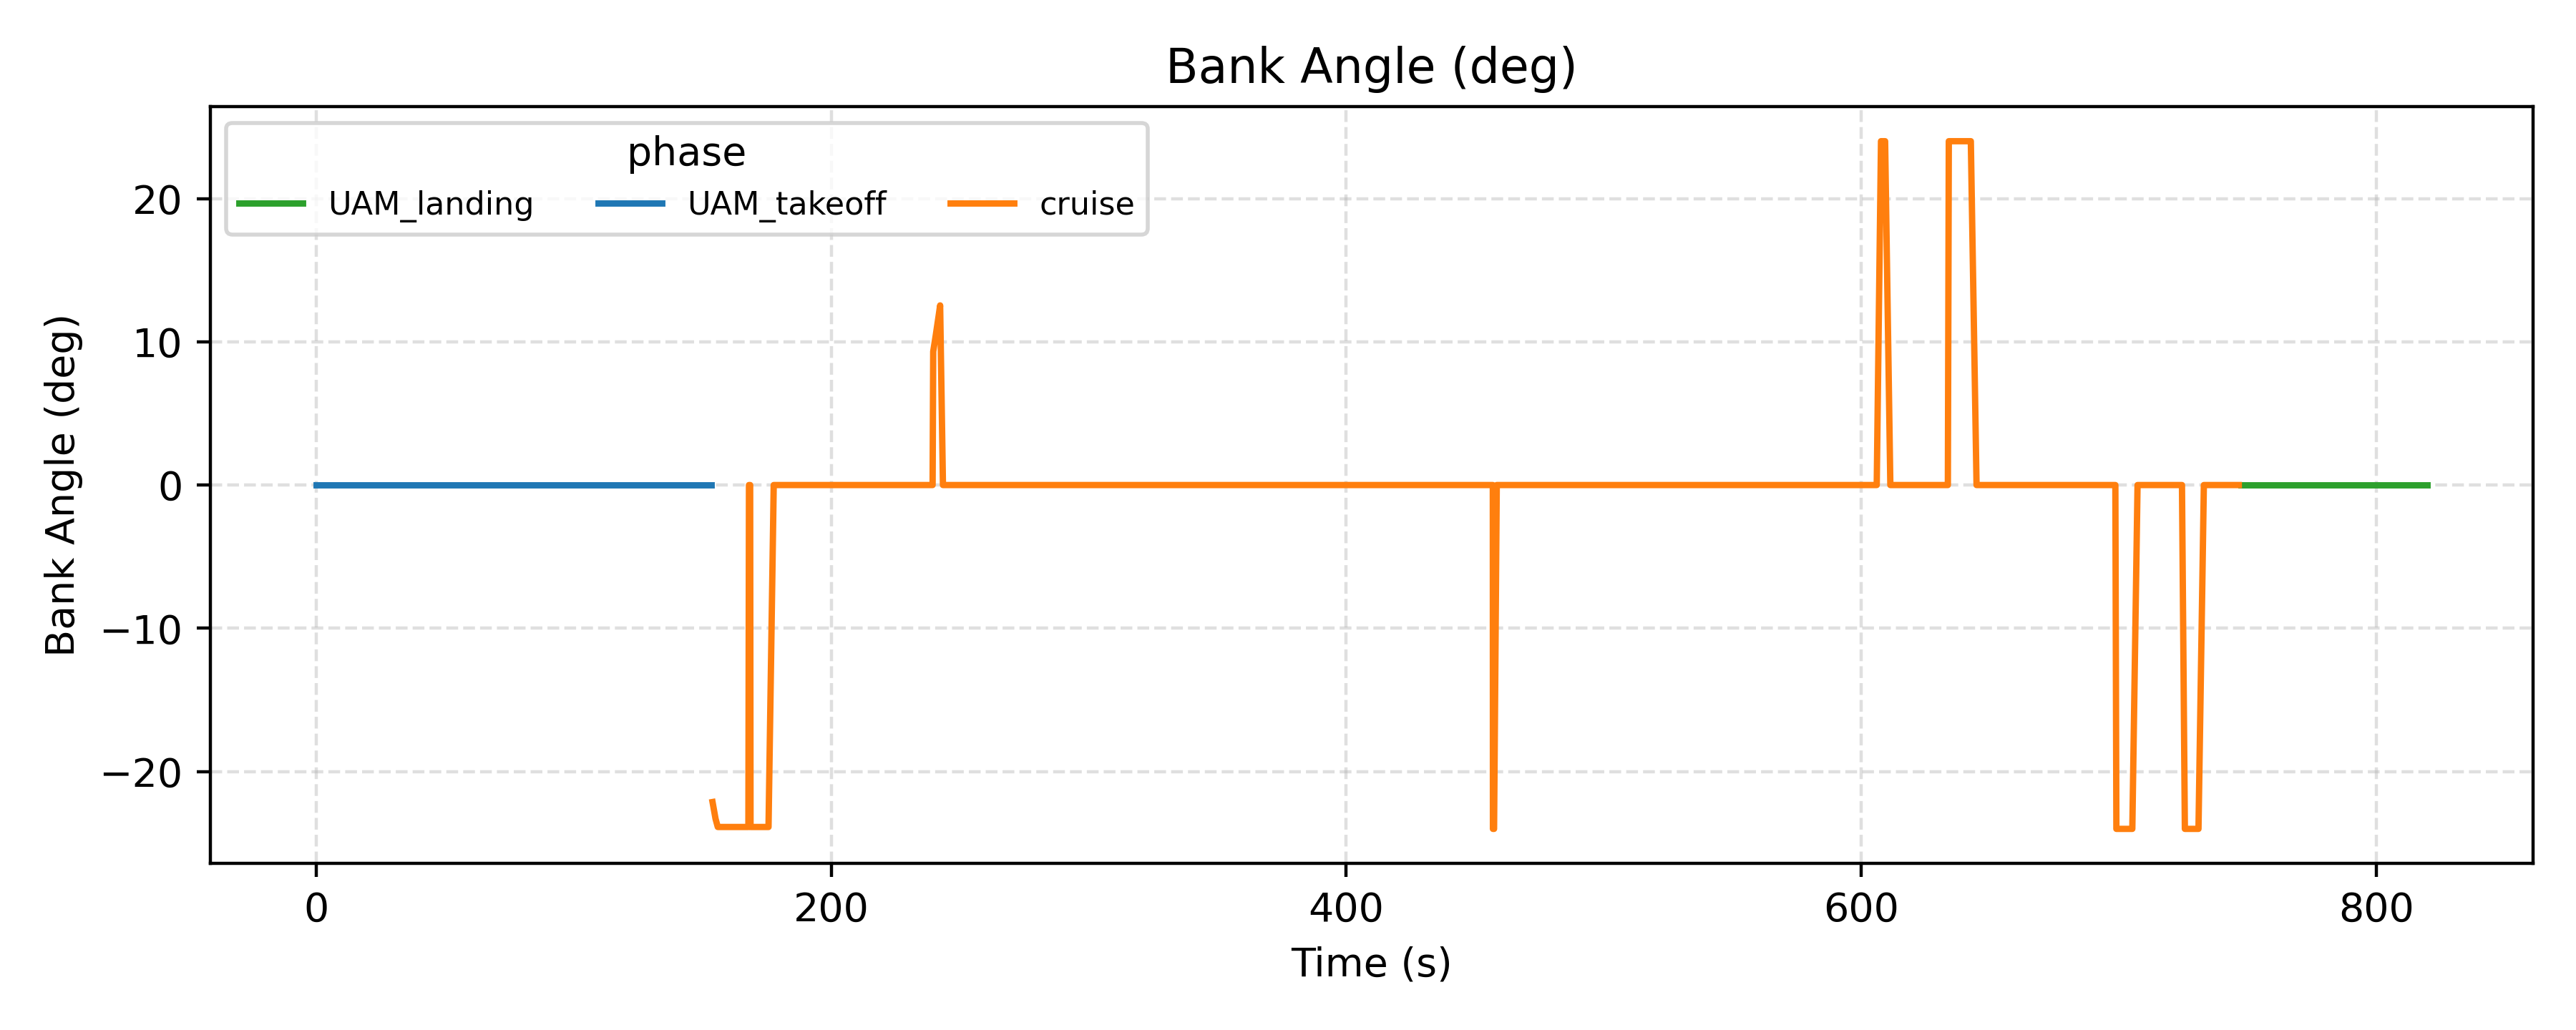
\includegraphics[width=0.86\textwidth]{results/trajectoryB_bank.png}
  \caption{Planned bank-angle profile $\phi(\tau)$ for Trajectory B (deg).}
  \label{fig:trajB_bank}
\end{figure}

\subsubsection*{Summary Statistics}
\begin{table}[H]
  \centering
  \caption{Summary statistics for the planned reference Trajectory B.}
  \label{tab:trajB_summary}
  \begin{tabular}{l r}
    \toprule
    Points & \num{500} \\
    Total time $T$ (s) & \num{819.81} \\
    Total time $T$ (min) & \num{13.66} \\
    Total distance $L$ (km) & \num{13.79} \\
    Mean TAS (m/s) & \num{16.67} \\
    Peak bank angle $\max \phi$ (deg) & \num{24.01} \\
    Peak turn rate $\max \dot{\psi}$ (deg/s) & \num{16.68} \\
    Peak climb rate $\max \dot{H}$ (m/s) & \num{6.63} \\
    \bottomrule
  \end{tabular}
\end{table}

\section{Conflict Handling}
\label{sec:results_conflicts}

In this section, the ability of the framework to detect and resolve conflicts is demonstrated.
Two representative trajectories were selected within the Hamburg corridor network
(trajectory \texttt{HAM~$\rightarrow$~WILH} and trajectory \texttt{TTNB~$\rightarrow$~HOHE}),
whose initially planned routes overlap spatially and temporally. This setup provides
a suitable test case for illustrating both the detection of a conflict and its
subsequent resolution through lateral re-routing.

\subsection{Conflict Detection}
The candidate routes were submitted to the NDMap conflict detection module
(Sec.~\ref{sec:ndmap}), which evaluates trajectory pairs in four-dimensional space
(longitude, latitude, altitude, time).  
Figure~\ref{fig:conflict_initial} shows the initially planned routes,
with the overlapping edge segment highlighted in red.  
NDMap reported a conflict interval
\([\tau_{\text{start}}, \tau_{\text{end}}] = [654.2\,\text{s}, 664.8\,\text{s}]\),
indicating that both UAM trajectories would occupy the same corridor segment
within a temporal overlap of approximately \SI{10.6}{s}.

\begin{figure}[H]
  \centering
  \begin{subfigure}[t]{0.48\textwidth}
    \centering
    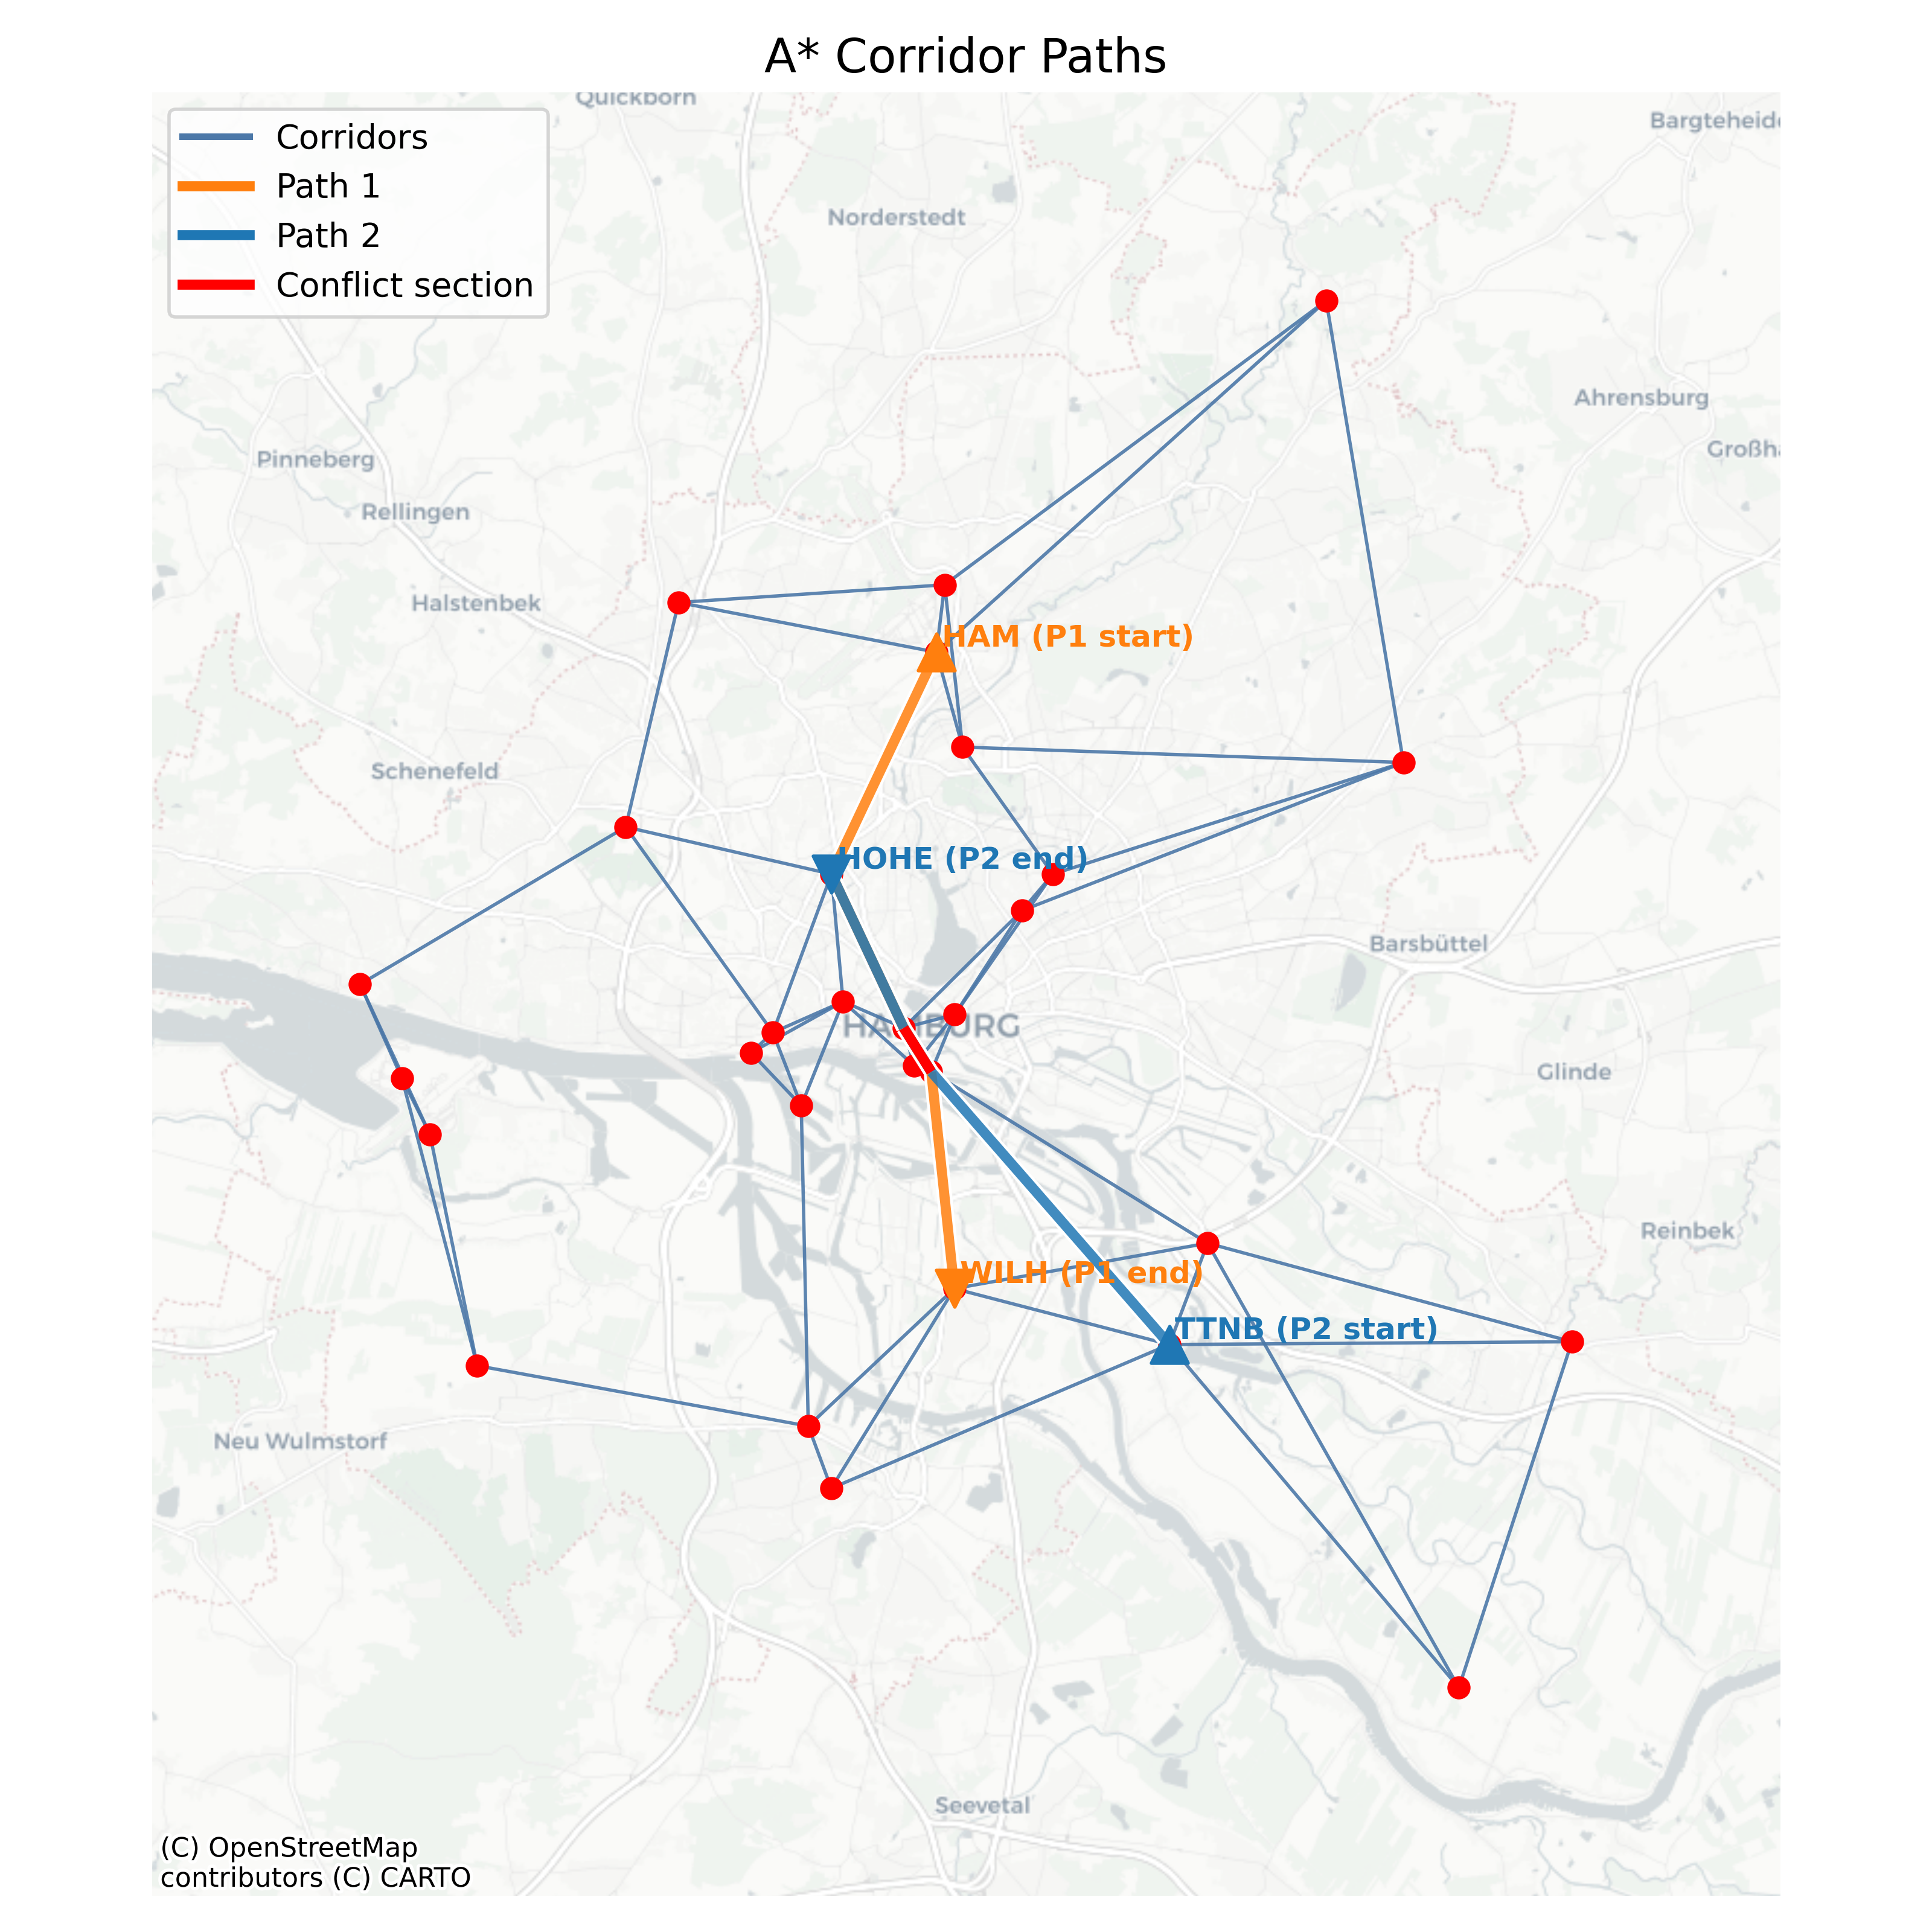
\includegraphics[width=\textwidth]{results/corridors_multiple_paths.png}
    \caption{Initial planned routes for \texttt{HAM~$\rightarrow$~WILH} and \texttt{TTNB~$\rightarrow$~HOHE}; the overlapping planned corridor segment (conflict) is marked in red.}
    \label{fig:conflict_initial}
  \end{subfigure}
  \hfill
  \begin{subfigure}[t]{0.48\textwidth}
    \centering
    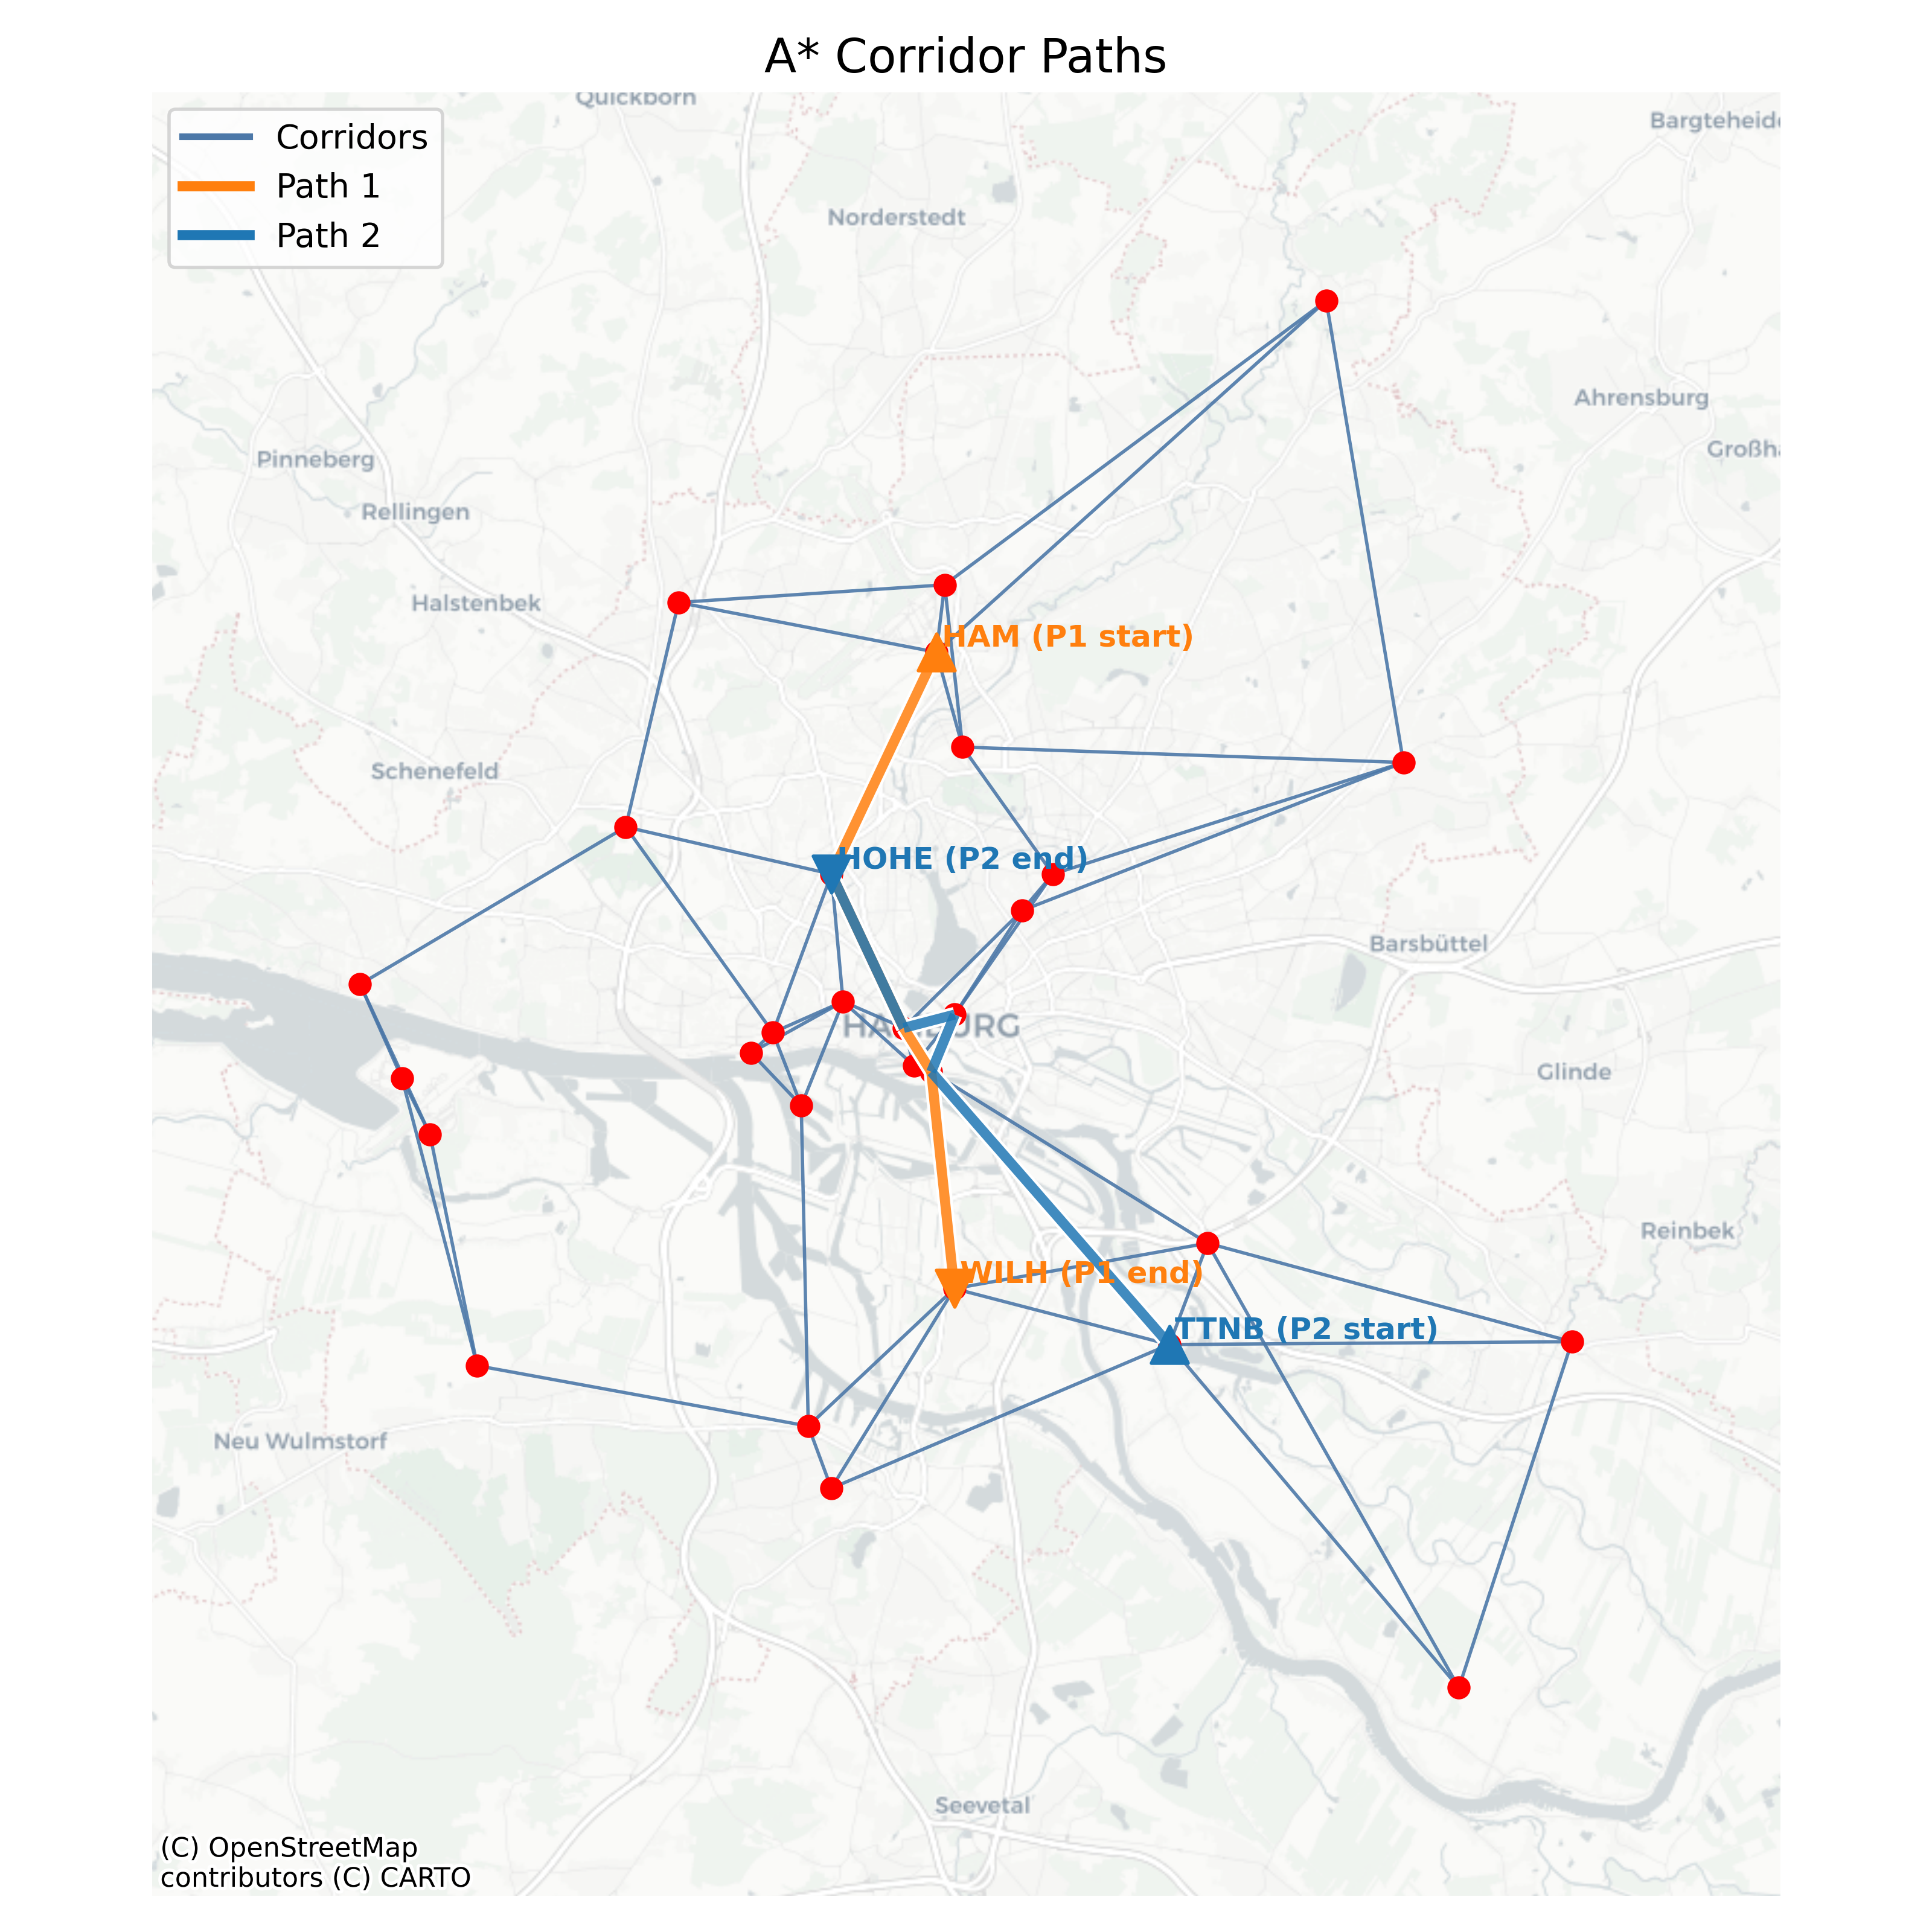
\includegraphics[width=\textwidth]{results/corridors_multiple_paths_resolved.png}
    \caption{Re-planned conflict-free route for \texttt{TTNB~$\rightarrow$~HOHE}; the revised planned path avoids the previously conflicting corridor.}
    \label{fig:conflict_resolved}
  \end{subfigure}
  \caption{Comparison of conflict detection and resolution using NDMap and rerouting on planned routes.}
  \label{fig:conflict_comparison}
\end{figure}

\subsection{Conflict Resolution}
To resolve the detected conflict, the integrated rerouting strategy within the path
planning framework (Sec.~\ref{sec:astar_global}) was applied.  
Edges involved in the conflict were temporarily penalized by assigning
infinite cost in the corridor graph, effectively discouraging their selection
in subsequent planning iterations. A new A* search was then performed
for the affected trajectory (\texttt{TTNB~$\rightarrow$~HOHE}), yielding
a longer but conflict-free path.  
The outcome is shown in Fig.~\ref{fig:conflict_resolved}, where the rerouted
trajectory bypasses the overlapping corridor segment, thereby eliminating
the temporal and spatial conflict.

\subsection*{Summary}
This case study demonstrates the integrated conflict handling approach of the framework:
conflicts are detected via NDMap (Sec.~\ref{sec:ndmap}), and if present,
the route is adaptively recomputed by modifying corridor edge weights and re-running
A* search (Sec.~\ref{sec:astar_global}).  
Although this may increase the total distance and travel time, the resulting trajectory
is conflict-free, supporting safe and scalable multi-UAM operations within the Hamburg
scenario.

\subsection{Conflict Handling with Interchanged Endpoints}
A second case study considers two trajectories with interchanged start and end
vertiports: trajectory \texttt{HARB~$\rightarrow$~TTNB} and
trajectory \texttt{TTNB~$\rightarrow$~HARB}.  
In the initial planning stage, both trajectories select the same shortest route,
leading to a complete overlap of the corridor segment between the two vertiports.  
This results in an unavoidable spatial and temporal conflict when both plans are
submitted simultaneously.

\subsubsection*{Conflict Detection and Resolution}
Figure~\ref{fig:conflict_interchanged} compares the initial conflicting routes
(left) with the resolved case (right). NDMap (Sec.~\ref{sec:ndmap}) flagged the
overlapping corridor segment (red) as a conflict, with simultaneous occupancy
intervals for both trajectories.  
To resolve this, the integrated rerouting strategy (Sec.~\ref{sec:astar_global})
was applied: the conflicting edge was penalized by assigning it infinite cost,
and a new A* search was run for the later-submitted trajectory
(\texttt{TTNB~$\rightarrow$~HARB}).  
The new solution yields the second-shortest path in the network, which avoids
the overlapping corridor and ensures conflict-free operation.

\begin{figure}[H]
  \centering
  \begin{subfigure}[t]{0.48\textwidth}
    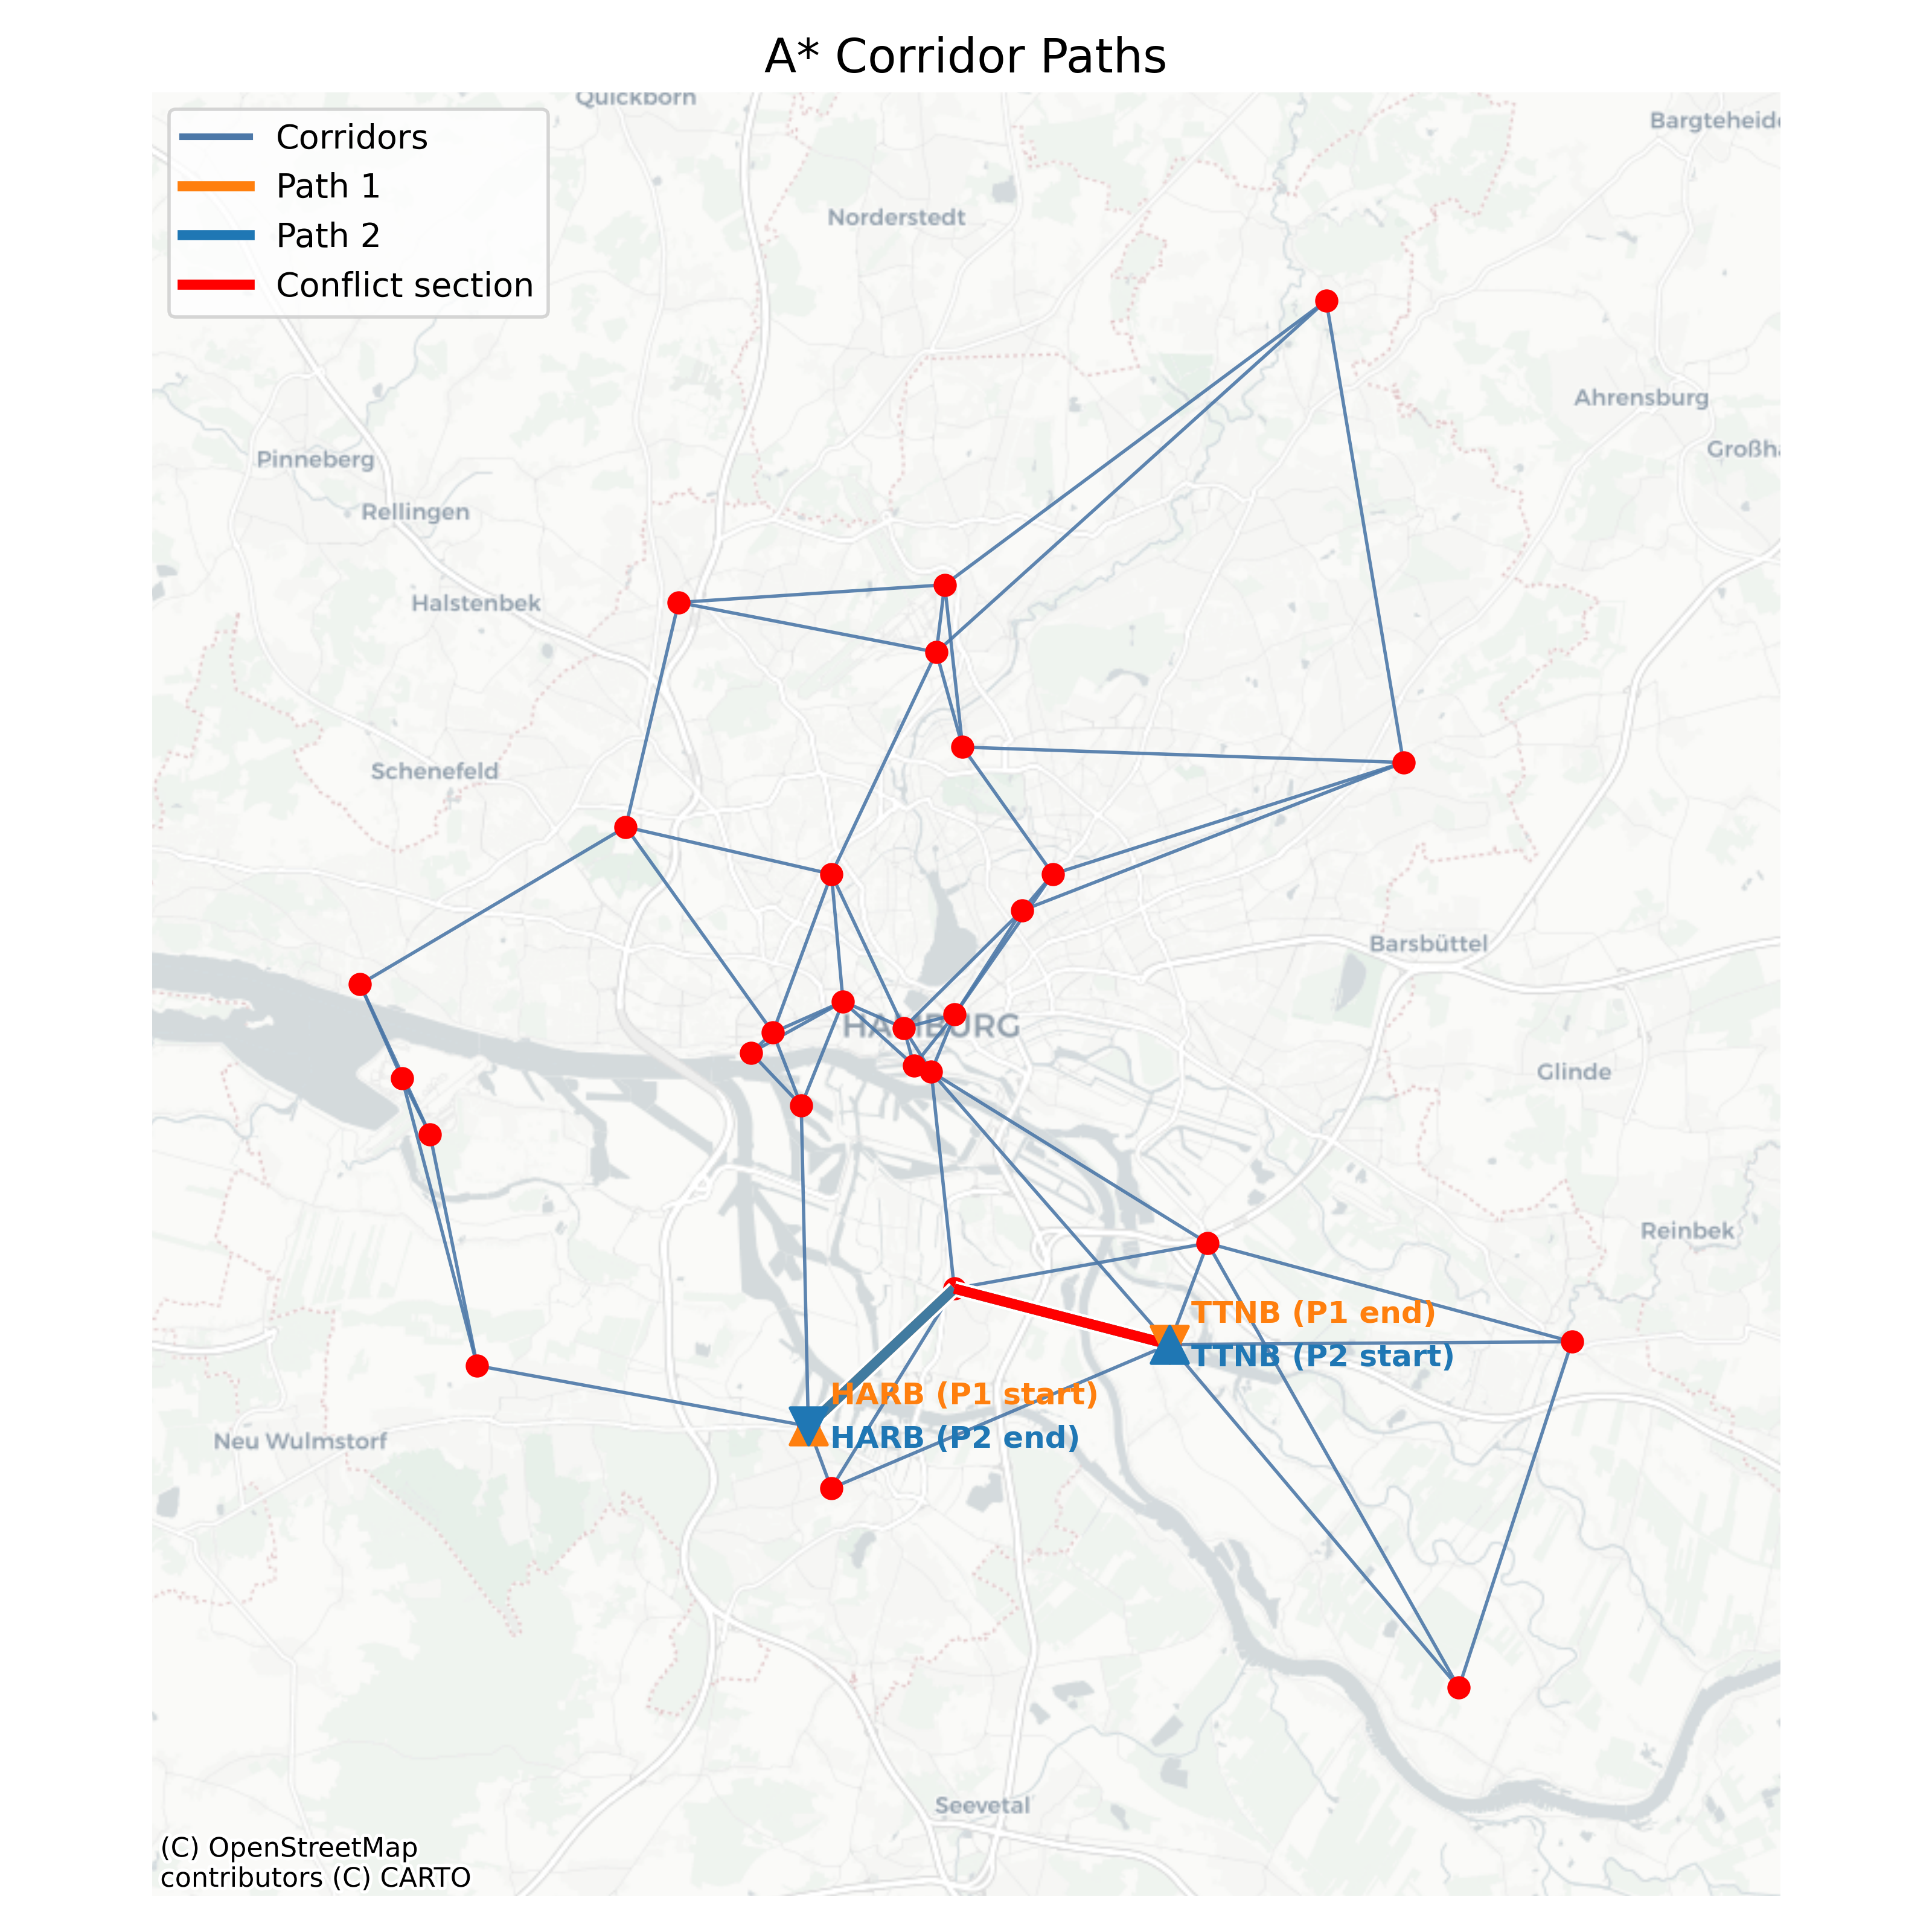
\includegraphics[width=\textwidth]{results/corridors_multiple_paths_1.png}
    \caption{Initial planned routes for interchanged endpoints: both planned paths overlap completely on the shortest corridor segment (conflict).}
    \label{fig:conflict_interchanged_initial}
  \end{subfigure}
  \hfill
  \begin{subfigure}[t]{0.48\textwidth}
    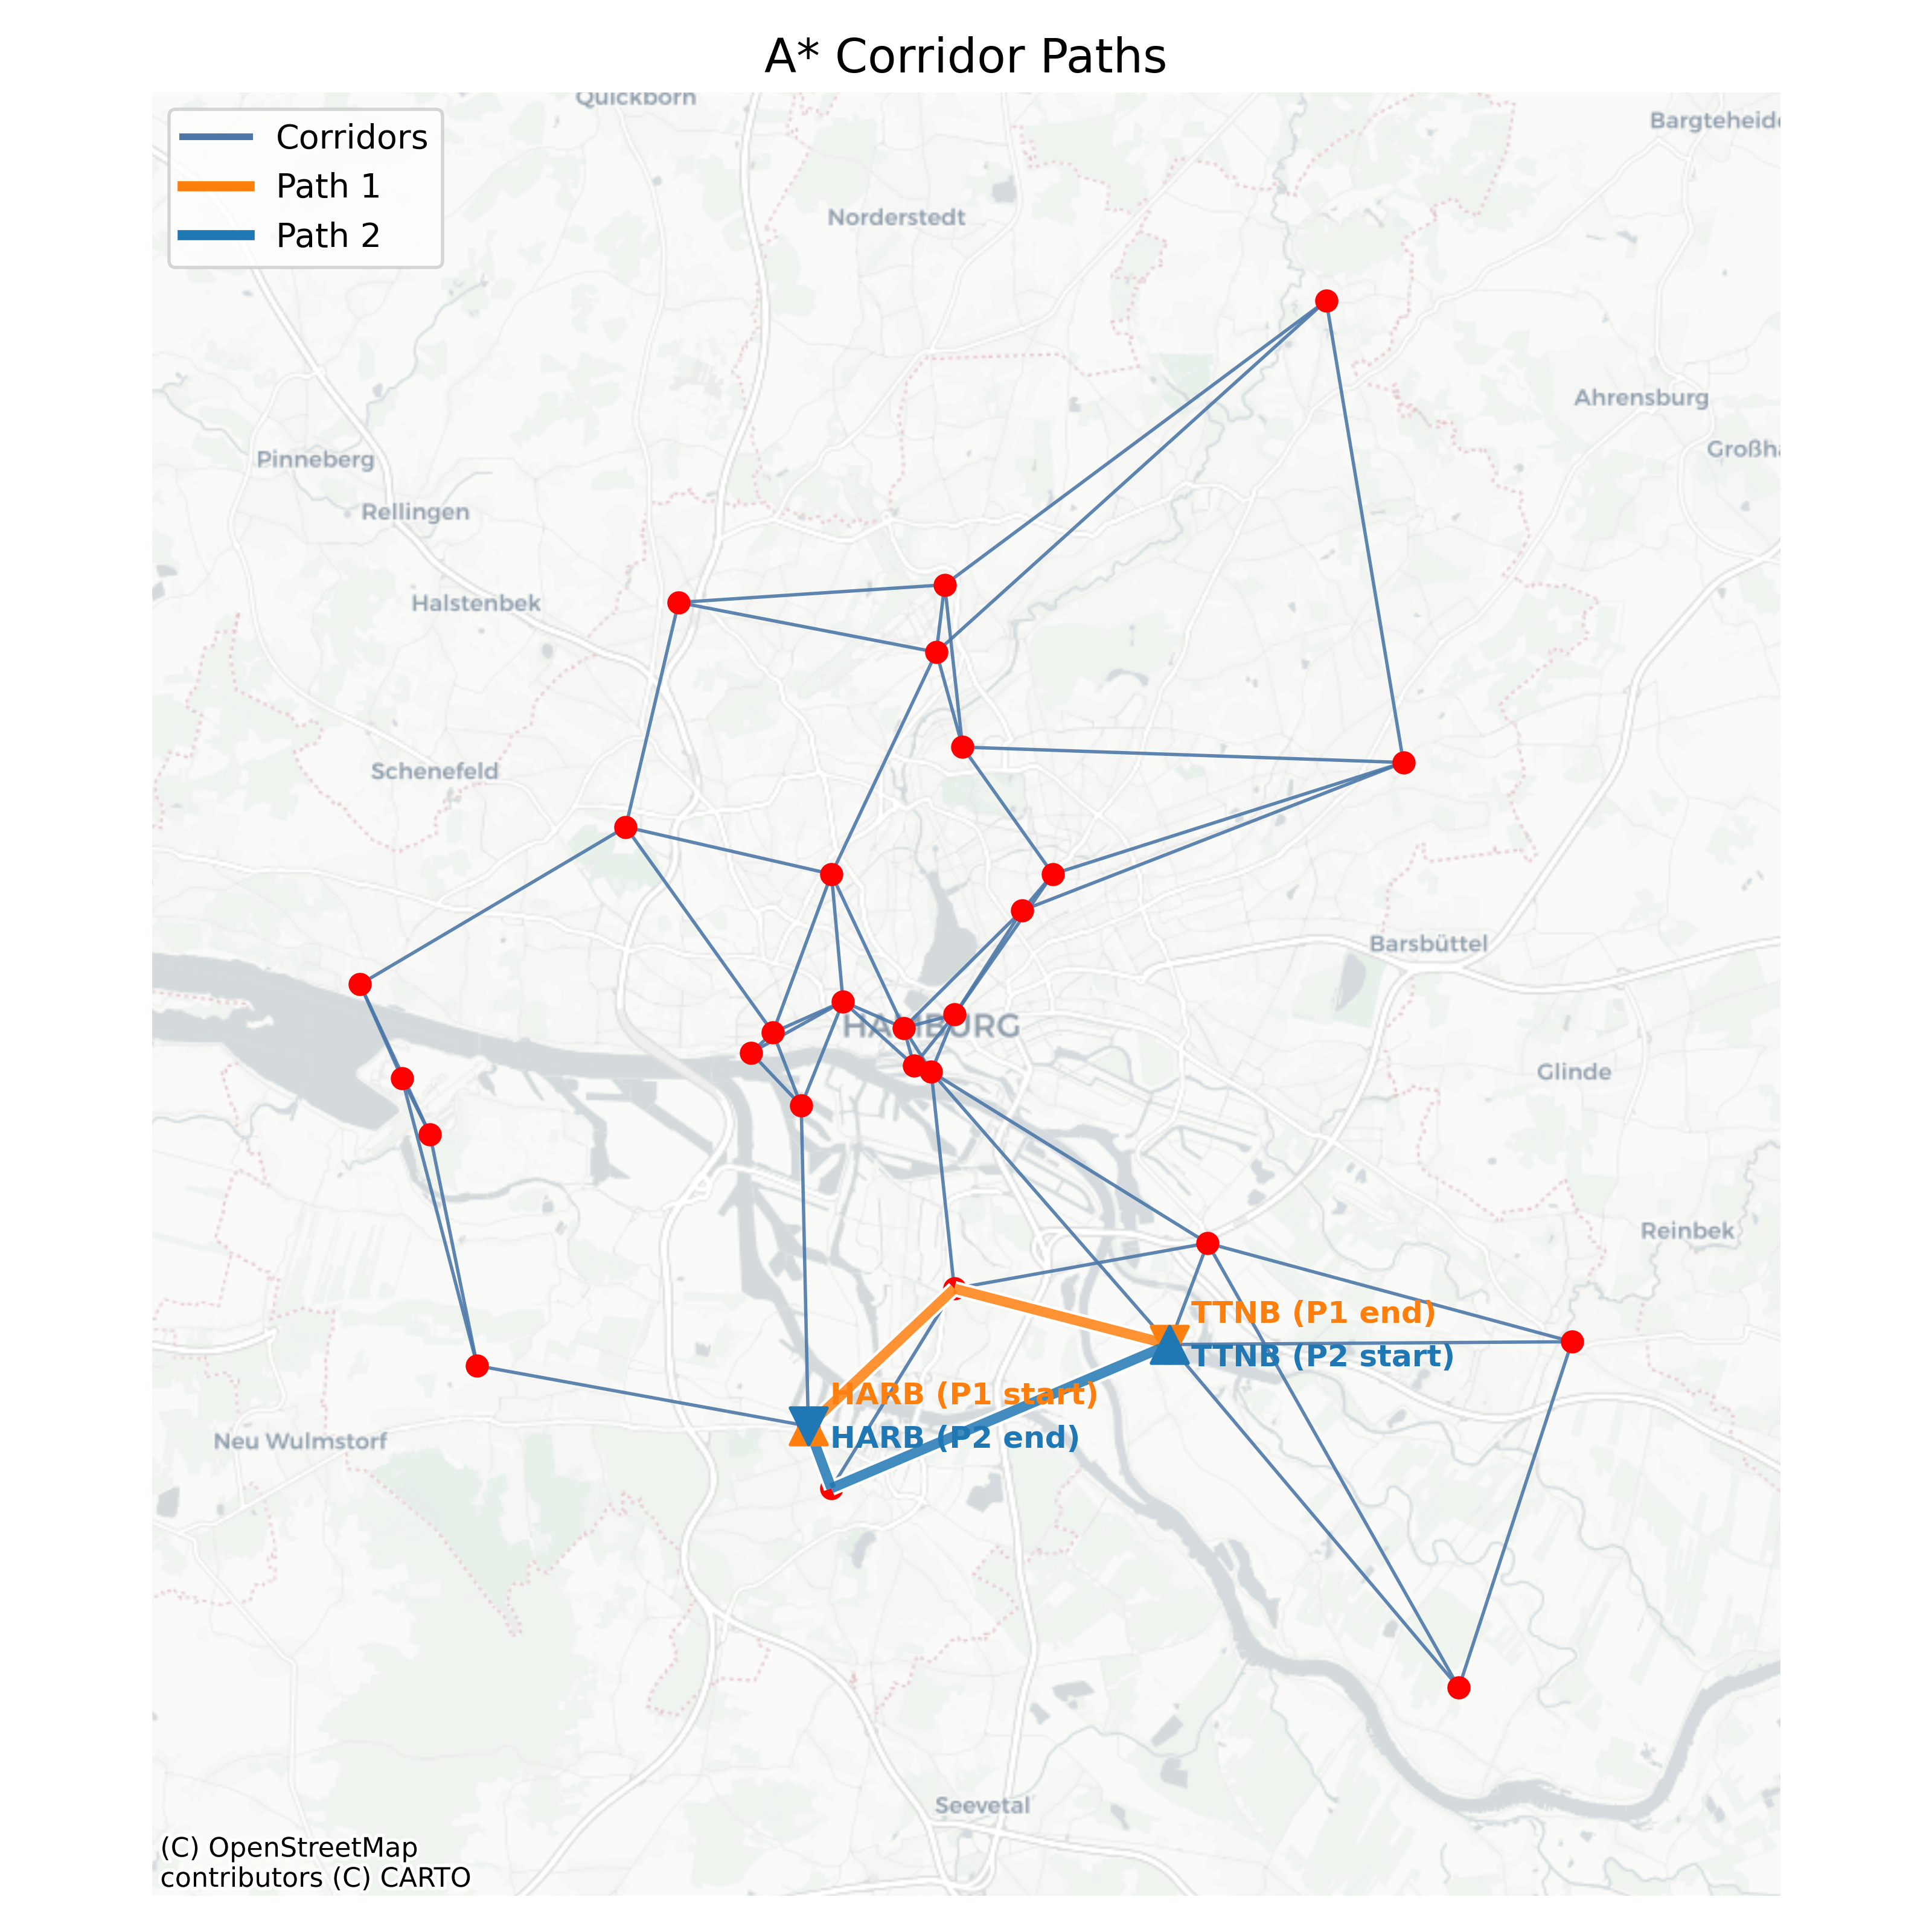
\includegraphics[width=\textwidth]{results/corridors_multiple_paths_resolved_1.png}
    \caption{Re-planned conflict-free route for \texttt{TTNB~$\rightarrow$~HARB} along the second-shortest corridor path, eliminating overlap.}
    \label{fig:conflict_interchanged_resolved}
  \end{subfigure}
  \caption{Conflict handling for interchanged endpoints on planned routes.  
           The later trajectory is re-planned to avoid the overlapping corridor.}
  \label{fig:conflict_interchanged}
\end{figure}

\subsubsection*{Summary}
This case demonstrates the robustness of the rerouting mechanism in situations
where direct shortest paths are infeasible due to complete overlap.
By enforcing the second-shortest path in the graph, the framework maintains
safety while preserving operational feasibility in dense urban networks.

\section{Scalability Evaluation with 100 Trajectories}
\label{sec:scalability_eval}

To assess the computational scalability of the proposed framework, a batch of
100 synchronous trajectory requests was processed. In this setup, each request
was completed before the next one was started. Independent pairs of take-off
and landing vertiports were randomly selected, and successful trajectories were
used for evaluation. Conflict detection and resolution mechanisms were disabled
in this experiment to isolate the baseline computational performance.

\subsection*{Summary Statistics}
The mean and standard deviation of the measured runtimes across the 100 test cases are summarized in Table~\ref{tab:runtime_100}. 
The 100 cases used distinct pairs of take-off and landing vertiports within the Hamburg vertiport network employed in this study, whose corridor graph was fully connected. Because conflict resolution was disabled for this evaluation and the graph connectivity guaranteed a path between any pair, all 100 planned trajectories were successfully generated.

\begin{table}[H]
  \centering
  \caption{Runtime summary over 100 synchronous trajectory requests.}
  \label{tab:runtime_100}
  \begin{tabular}{l r r}
    \toprule
    Metric & Mean (ms) & Std (ms) \\
    \midrule
    Total time              & 162.92 & 38.38 \\
    Trajectory generation   & 151.43 & 38.06 \\
    A* path finding         & 0.41   & 1.21  \\
    \bottomrule
  \end{tabular}
\end{table}

\subsection*{Scatter Plot Analysis}
Figure~\ref{fig:astar_vs_nodes} shows the relationship between A* runtime and \emph{path nodes (count)}. 
No meaningful correlation was observed (e.g., $r\approx0.02$), confirming that A* search latency is essentially independent of the number of nodes traversed.  
In contrast, Fig.~\ref{fig:trajgen_vs_nodes} demonstrates a strong positive correlation (e.g., $r\approx0.75$) 
between \emph{path nodes (count)} and trajectory generation time, consistent with the generator’s per-segment workload.

\begin{figure}[H]
  \centering
  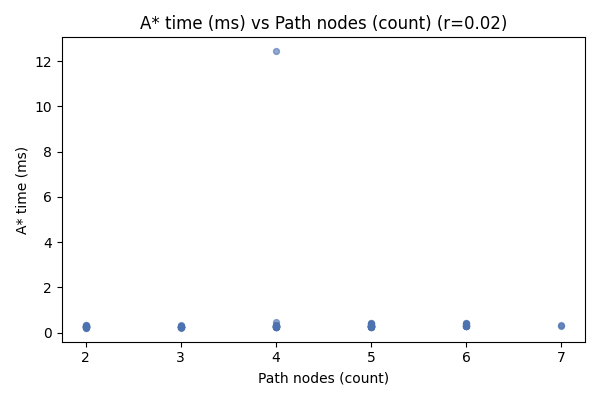
\includegraphics[width=0.7\textwidth]{results/scatter_astar_vs_nodes.png}
  \caption{A* runtime vs.~path nodes (count). Example correlation: $r\approx0.02$.}
  \label{fig:astar_vs_nodes}
\end{figure}

\begin{figure}[H]
  \centering
  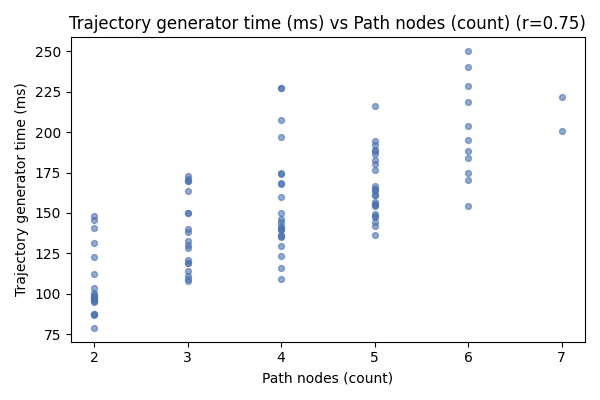
\includegraphics[width=0.7\textwidth]{results/scatter_traj_generator_vs_nodes.png}
  \caption{Trajectory generator runtime vs.~path nodes (count). Example correlation: $r\approx0.75$.}
  \label{fig:trajgen_vs_nodes}
\end{figure}

\subsection*{Runtime Distributions}
The distribution of total processing time across the 100 runs is shown in
Fig.~\ref{fig:hist_total}, with values concentrated in the \SIrange{120}{260}{ms} range. 
The distribution of trajectory generation runtimes (Fig.~\ref{fig:hist_trajgen})
shows a similar pattern, confirming that trajectory generation is the dominant
contributor to total latency.

\begin{figure}[H]
  \centering
  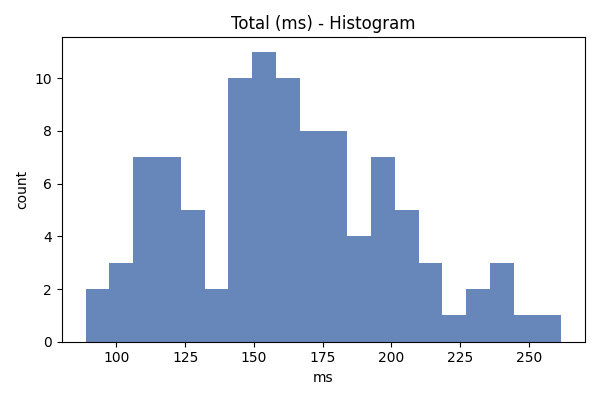
\includegraphics[width=0.7\textwidth]{results/dist_total_ms.png}
  \caption{Histogram of total runtime per trajectory request.}
  \label{fig:hist_total}
\end{figure}

\begin{figure}[H]
  \centering
  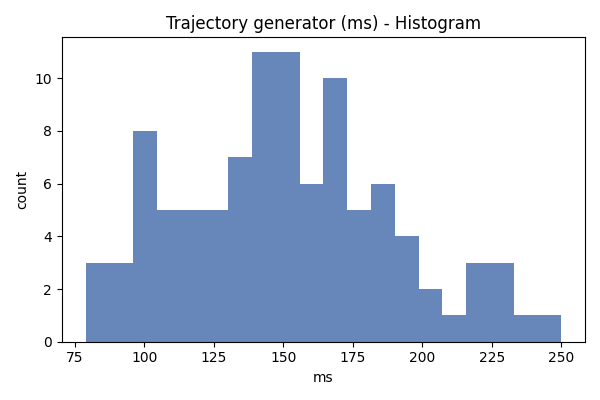
\includegraphics[width=0.7\textwidth]{results/dist_traj_generator_ms.png}
  \caption{Histogram of trajectory generation runtime per request.}
  \label{fig:hist_trajgen}
\end{figure}

\subsection*{Discussion}
These results demonstrate that the A* stage contributes negligibly to total latency,
with mean runtimes well below \SI{1}{ms} across the sampled path sizes. In contrast,
trajectory generation dominates the runtime and increases with the number of path
nodes (and thus legs to synthesize).  
Overall processing times of roughly \SI{160}{ms} per request indicate that the framework
can support real-time urban air mobility (UAM) trajectory planning in a synchronous,
single-request setting. Scaling to parallel, high-volume scenarios will require further
evaluation under active conflict detection and resolution.


\section{Evaluation under Active Conflict Resolution}
\label{sec:results_conflict_eval}

In addition to the synchronous evaluation without conflict detection and resolution (Sec.~\ref{sec:scalability_eval}), 
the framework was further assessed under active conflict handling. 
Fifteen random takeoff–landing pairs were selected from the Hamburg corridor network. 
For each path request, the conflict detection module (Sec.~\ref{sec:ndmap}) and the lateral re-routing strategy (Sec.~\ref{sec:results_conflicts}) 
were engaged. This setup allows measuring the combined latency of A* search, trajectory generation, and any re-planning iterations 
required to produce a conflict-free trajectory.

\subsection{Processing Strategy}
All 15 trajectory requests were processed synchronously, i.e.\ each request was completed 
before the next one started. This mode isolates the latency of the path-planning pipeline 
without concurrent scheduling effects. If NDMap detected a conflict, the edges involved 
were penalized and A* was re-run (Sec.~\ref{sec:results_conflicts}), which may yield 
longer paths and increased runtimes. Two cases could not be resolved by lateral re-routing alone and remained in conflict, 
indicating that an alternative strategy (e.g.\ altitude change or departure delay) would be necessary.

\subsection{Timing Results}
Across the 13 successfully resolved trajectories, the total end-to-end latency 
(from path request to final 4D trajectory) exhibited a wide spread:
\begin{itemize}
  \item \textbf{Count:} 13 trajectories,
  \item \textbf{Mean total time:} \SI{5286.19}{ms},
  \item \textbf{Standard deviation:} \SI{8003.16}{ms}.
\end{itemize}
Two effects plausibly contribute to this variance: (i) the statistics are based on a small sample (\(n=13\)), which makes the estimate of dispersion sensitive to a few long-running cases; and (ii) part of the measured duration includes inter-service I/O overhead, since trajectory samples are exchanged via intermediate files rather than through an in-process interface.

Figure~\ref{fig:conflict_eval_scatter} shows the scatter plot of total time versus 
path distance for these trajectories. A positive correlation \(r=0.76\) indicates that 
longer paths tend to require more processing time, reflecting both increased 
trajectory-generation cost and additional A* iterations in some cases.

\begin{figure}[H]
  \centering
  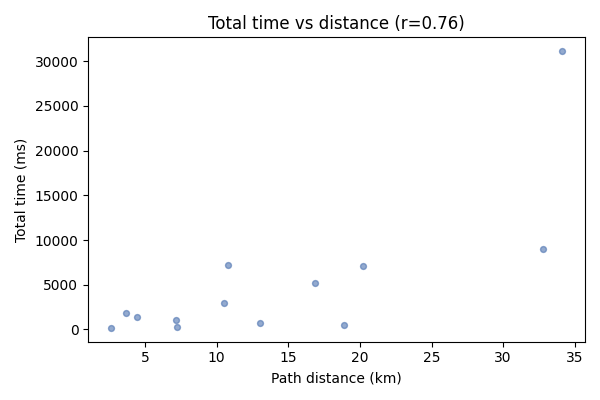
\includegraphics[width=0.48\textwidth]{results/scatter_total_vs_distance_conflicts.png}
  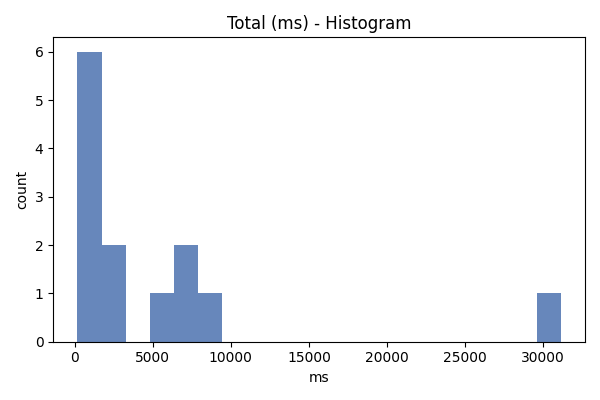
\includegraphics[width=0.48\textwidth]{results/dist_total_ms_conflicts.png}
  \caption{Left: total processing time versus path distance for 13 conflict-free planned trajectories.
           Right: histogram of total processing times across the same runs.}
  \label{fig:conflict_eval_scatter}
\end{figure}

\subsection{Discussion}
Compared to the evaluation without conflict resolution (Sec.~\ref{sec:scalability_eval}), 
both the mean latency and its variance are markedly higher under active conflict handling. 
This is expected, as each detected conflict triggers additional A* searches with modified 
edge weights (Sec.~\ref{sec:results_conflicts}), potentially increasing path length 
and computation time. The two unresolved cases underscore the need for 
more flexible resolution mechanisms—such as altitude assignment, departure delay, or 
risk-map based edge re-weighting—to handle complex conflicts where lateral re-routing alone 
cannot find a feasible solution.

\medskip
\noindent
This evaluation thus highlights the trade-off between safety and responsiveness: 
while lateral re-routing enables automatic deconfliction in many scenarios, 
its runtime cost scales with graph complexity and the number of iterations required.
The observed variance is further influenced by the small sample size and by the current file-based exchange between services; tighter in-process coupling (e.g., integrating CFMS into the planner) would plausibly reduce such overhead.


  \chapter{Conclusions and Future Work}
\label{s_conclusions}

\section{Conclusions}
This thesis has presented the design, implementation, and evaluation of a
microservice-based path planning framework for urban air mobility (UAM)
operations. By decomposing the system into independent services, the planner
was able to integrate heterogeneous components implemented in different
languages and tools—namely, the A* global planner (Python), the CFMS trajectory
generator (C++), and the NDMap conflict detection module (C++). This modular
design demonstrates the potential of microservices for building scalable and
extensible architectures for U-space operations.

The framework was evaluated using a representative vertiport and corridor
network modeled over the metropolitan area of Hamburg. Experiments focused on
quantifying delays at different processing stages, including A* path finding,
trajectory generation, and overall end-to-end response time. Results showed
that:
\begin{itemize}
    \item The A* path finding step contributed negligibly to the total delay,
    with runtimes consistently below 1~ms.
    \item Trajectory generation dominated the computational cost, with runtimes
    scaling linearly with path distance.
    \item The total processing time per trajectory request was on the order of
    200~ms, demonstrating the feasibility of near real-time operation for
    single-request scenarios.
    \item Conflict detection and resolution were successfully demonstrated using
    NDMap, with lateral rerouting as the chosen strategy to avoid overlapping
    trajectories.
\end{itemize}

Overall, the system provides a primitive but functional prototype of a path
planner for UAM operations, highlighting both the feasibility and the
challenges of integrating multiple specialized modules into a unified framework.

\section{Future Work}
While the present study establishes a foundation, several extensions are
necessary to bring the framework closer to realistic deployment:

\subsection*{Enhanced Conflict Resolution}
The current work focused exclusively on lateral rerouting through penalization
of conflicting edges in the corridor graph. Future extensions should include
additional resolution strategies such as:
\begin{itemize}
    \item \textbf{Temporal deconfliction:} delaying departure times to avoid
    simultaneous use of a corridor.
    \item \textbf{Vertical deconfliction:} assigning different altitude layers
    to conflicting trajectories.
    \item \textbf{Hybrid strategies:} combining lateral, temporal, and vertical
    maneuvers to balance efficiency and safety.
\end{itemize}

\subsection*{Complex Airspace Modeling}
The current corridor network was static, uniform in altitude, and of fixed
width. Future studies should incorporate:
\begin{itemize}
    \item Multiple altitude layers with dynamic assignment,
    \item Variable corridor widths depending on traffic density or risk,
    \item More realistic urban scenarios with larger networks and higher traffic
    volumes.
\end{itemize}

\subsection*{Incorporation of External Factors}
To better approximate real-world operations, future versions should integrate:
\begin{itemize}
    \item \textbf{Weather effects:} wind, turbulence, and no-fly zones affecting
    edge weights and feasibility.
    \item \textbf{Risk maps:} penalizing corridors near sensitive areas (schools,
    hospitals, etc.) to reflect societal and regulatory constraints.
    \item \textbf{Dynamic re-weighting:} adjusting corridor costs in real time
    based on environmental and operational factors.
\end{itemize}

\subsection*{Aircraft Performance Models}
The present study employed simplified kinematic constraints. For improved
fidelity, future work should model:
\begin{itemize}
    \item Performance envelopes specific to different eVTOL types,
    \item More detailed climb, descent, and turn dynamics,
    \item Energy consumption models for battery-electric aircraft.
\end{itemize}

\subsection*{Scalability and Multi-Agent Evaluation}
The synchronous evaluation with 100 independent trajectory requests provided
baseline performance characteristics. Future studies should investigate:
\begin{itemize}
    \item Asynchronous and parallel trajectory requests at scale,
    \item End-to-end system latency under high traffic densities.
\end{itemize}

\medskip
\noindent
In summary, this thesis demonstrates that a microservice-based approach to UAM
path planning is both technically feasible and computationally efficient for
baseline scenarios. Expanding the framework with more advanced conflict
resolution strategies, richer airspace and aircraft models, and larger-scale
evaluations will be critical steps toward enabling safe, scalable, and
realistic integration of UAM operations into the future air traffic management
ecosystem.


\end{mainContent}

%------------------------------------------------------------------------------
% Back matter

\begin{backMatter}

  % Optional – relevant mostly in case you received support from external
  % entities, such as other institutes, companies or individuals.
  %\makeatletter
\chapter*{\fsdthesis@labels@acknowledgementsTitle}
\addcontentsline{toc}{chapter}{\fsdthesis@labels@acknowledgementsTitle}
\makeatother

\iffsdthesisAnonymize{}
  % Protect the identity of persons involved in the work by clearing the
  % acknowledgements.
  (ACKNOWLEDGEMENTS)
\else
%------------------------------------------------------------------------------
% Content section

%------------------------------------------------------------------------------
\fi


  \makeBibliography{}

\end{backMatter}

\end{document}
